\chapter{Consistency Checks for Language Model Forecasters}
\label{chap:consistency-checks}

\chapterprovenance{Adapted from ``Consistency Checks for Language Model
Forecasters'' by Daniel Paleka, Abhimanyu Pallavi Sudhir, Alejandro Alvarez,
Vineeth Bhat, Adam Shen, Evan Wang, and Florian Tram\`er.}

%\newcommand{\rebuttal}[1]{\textcolor{red}{#1}}
\newcommand{\rebuttal}[1]{#1}
\newcommand{\rebuttaldeleted}[1]{}
\section*{Abstract}
Forecasting is a task that is difficult to evaluate: the ground truth can only be known in the future. Recent work showing LLM forecasters rapidly approaching human-level performance begs the question: how can we benchmark and evaluate these forecasters \textit{instantaneously}? Following the consistency check framework, we measure the performance of forecasters in terms of the consistency of their predictions on different logically-related questions. We propose a new, general consistency metric based on  \textit{arbitrage}: for example, if a forecasting AI illogically predicts that both the Democratic and Republican parties have 60\% probability of winning the 2024 US presidential election, an arbitrageur can trade against the forecaster's predictions and make a profit. We build an automated evaluation system that generates a set of base questions, instantiates consistency checks from these questions, elicits the predictions of the forecaster, and measures the consistency of the predictions. We then build a standard, proper-scoring-rule forecasting benchmark, and show that our (instantaneous) consistency metrics correlate with LLM forecasters' ground truth Brier scores (which are only known in the future). We also release a consistency benchmark that resolves in 2028, providing a long-term evaluation tool for forecasting.

\section{Introduction}

\emph{Prediction markets} are markets that pay out contingent on an event. For a market such as ``\$1 if Jeb Bush is elected President in 2028'', the price reflects the ``market estimate'' for the probability of that event. Prediction markets are a promising tool for aggregating information from disparate sources to arrive at the most correct possible belief after taking into account all relevant information \citep{arrowPromisePredictionMarkets2008, hansonLogarithmicMarketScoring2002}.


Until 2024, LLM forecasters generally performed poorly relative to human forecasters \citep{zouForecastingFutureWorld2022, schoeneggerLargeLanguageModel2023}.
However, recent works \citep{halawiApproachingHumanLevelForecasting2024, schoeneggerWisdomSiliconCrowd2024,safeai2024forecasters} suggest that LLM-based forecasters can rival human forecasts on forecasting websites such as Metaculus, PredictIt, and Manifold Markets.
%\citet{halawiApproachingHumanLevelForecasting2024} achieve this via retrieval-augmented generation (RAG) and fine-tuning, while \cite{schoeneggerWisdomSiliconCrowd2024} obtain consensus from a crowd of LLM forecasters.
%\manyuunimp{perhaps mention https://www.lesswrong.com/posts/uGkRcHqatmPkvpGLq/contra-papers-claiming-superhuman-ai-forecasting and references therein, including the Hendrycks paper people were criticizing}
%There is also an ongoing ``Humans vs Bots'' competition underway on Manifold Markets \cite{manifoldHumanBotsForecasting2024}
%\todo{idk if we want to cite the Scott Alexander blog post?}.

A key question emerges: \emph{once LLM forecasters are better than human ones, how can we efficiently evaluate their predictions?}
In particular, long-term forecasting questions are very important for decision-making \citep{tetlock2024longrange, lukemuehlhauserHowFeasibleLongrange2019}, and finding ground truth for evaluation in such contexts is infeasible by virtue of the questions resolving far in the future.

One approach, proposed by \citet{esmwcc}, is that even when we cannot evaluate the \emph{correctness} of LLM decisions, we can evaluate their \emph{logical consistency}.
For example, if an LLM forecaster gives probabilities 0.5 and 0.7 to ``Will Trump be elected US president?'' and ``Will someone other than Trump be elected US president?'', this is necessarily inconsistent.
\citet{esmwcc} demonstrated that GPT-4 and GPT-3.5-turbo, when asked one-sentence forecasting questions, were inconsistent on simple logical checks such as negation.

%\newpage

%\manyu{@dpaleka: describe our exact novelty against Fluri. Maybe also: (1) a bit longer of a spiel about consistency, training for consistency etc. (2) specific research questions e.g. does it correlate with ground truth, what if we just arbitraged the forecasts, etc.}
\begin{figure}[h]
    \begin{minipage}{0.55\textwidth}
    % First figure content
    \centering
    \vspace{-10pt}
    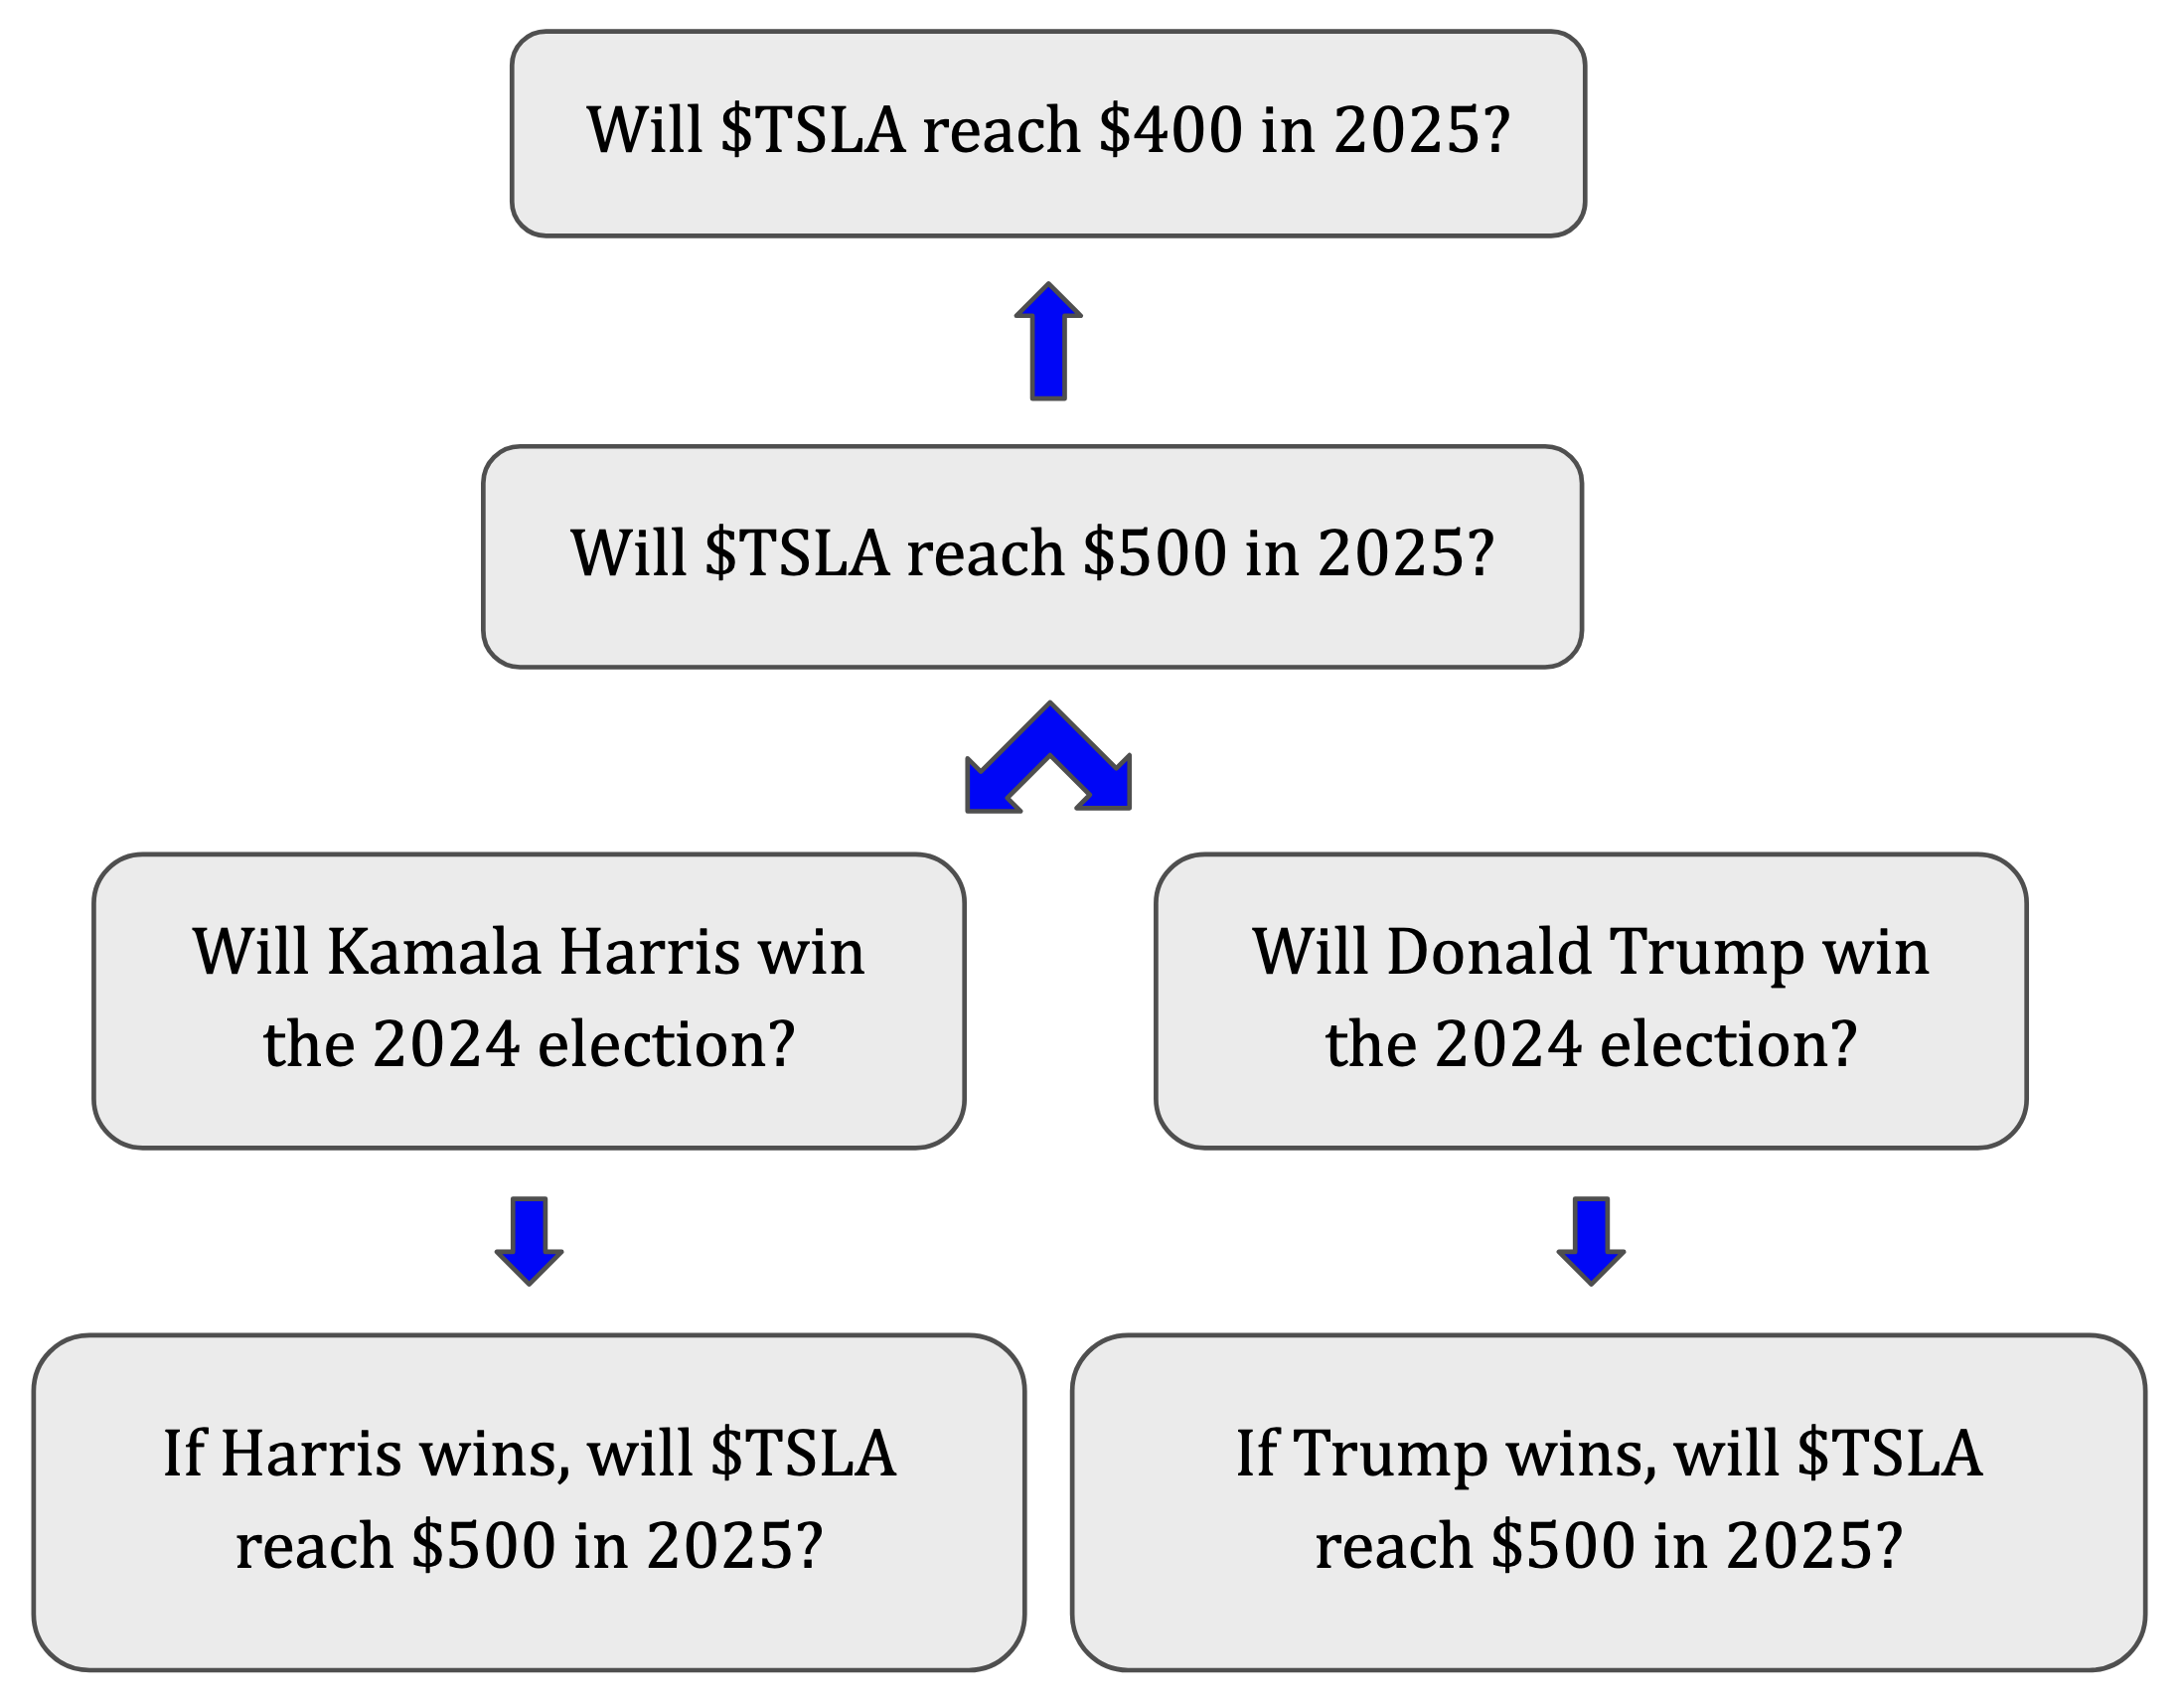
\includegraphics[width=\textwidth]{figures/consistency/fig1_short.png}
    \captionsetup{width=0.95\textwidth}
    \caption{
        Examples of
        %the \ConsequenceChecker{} and \ExpectedEvidenceChecker{}
        consistency check questions generated from the same question about Tesla stock reaching \$500 in 2025. The pipeline in \Cref{cfc/sec:pipeline} generates questions and evaluates a forecaster's consistency with respect to them.
    }
    \end{minipage}
    \hfill
    \begin{minipage}{0.44\textwidth}
    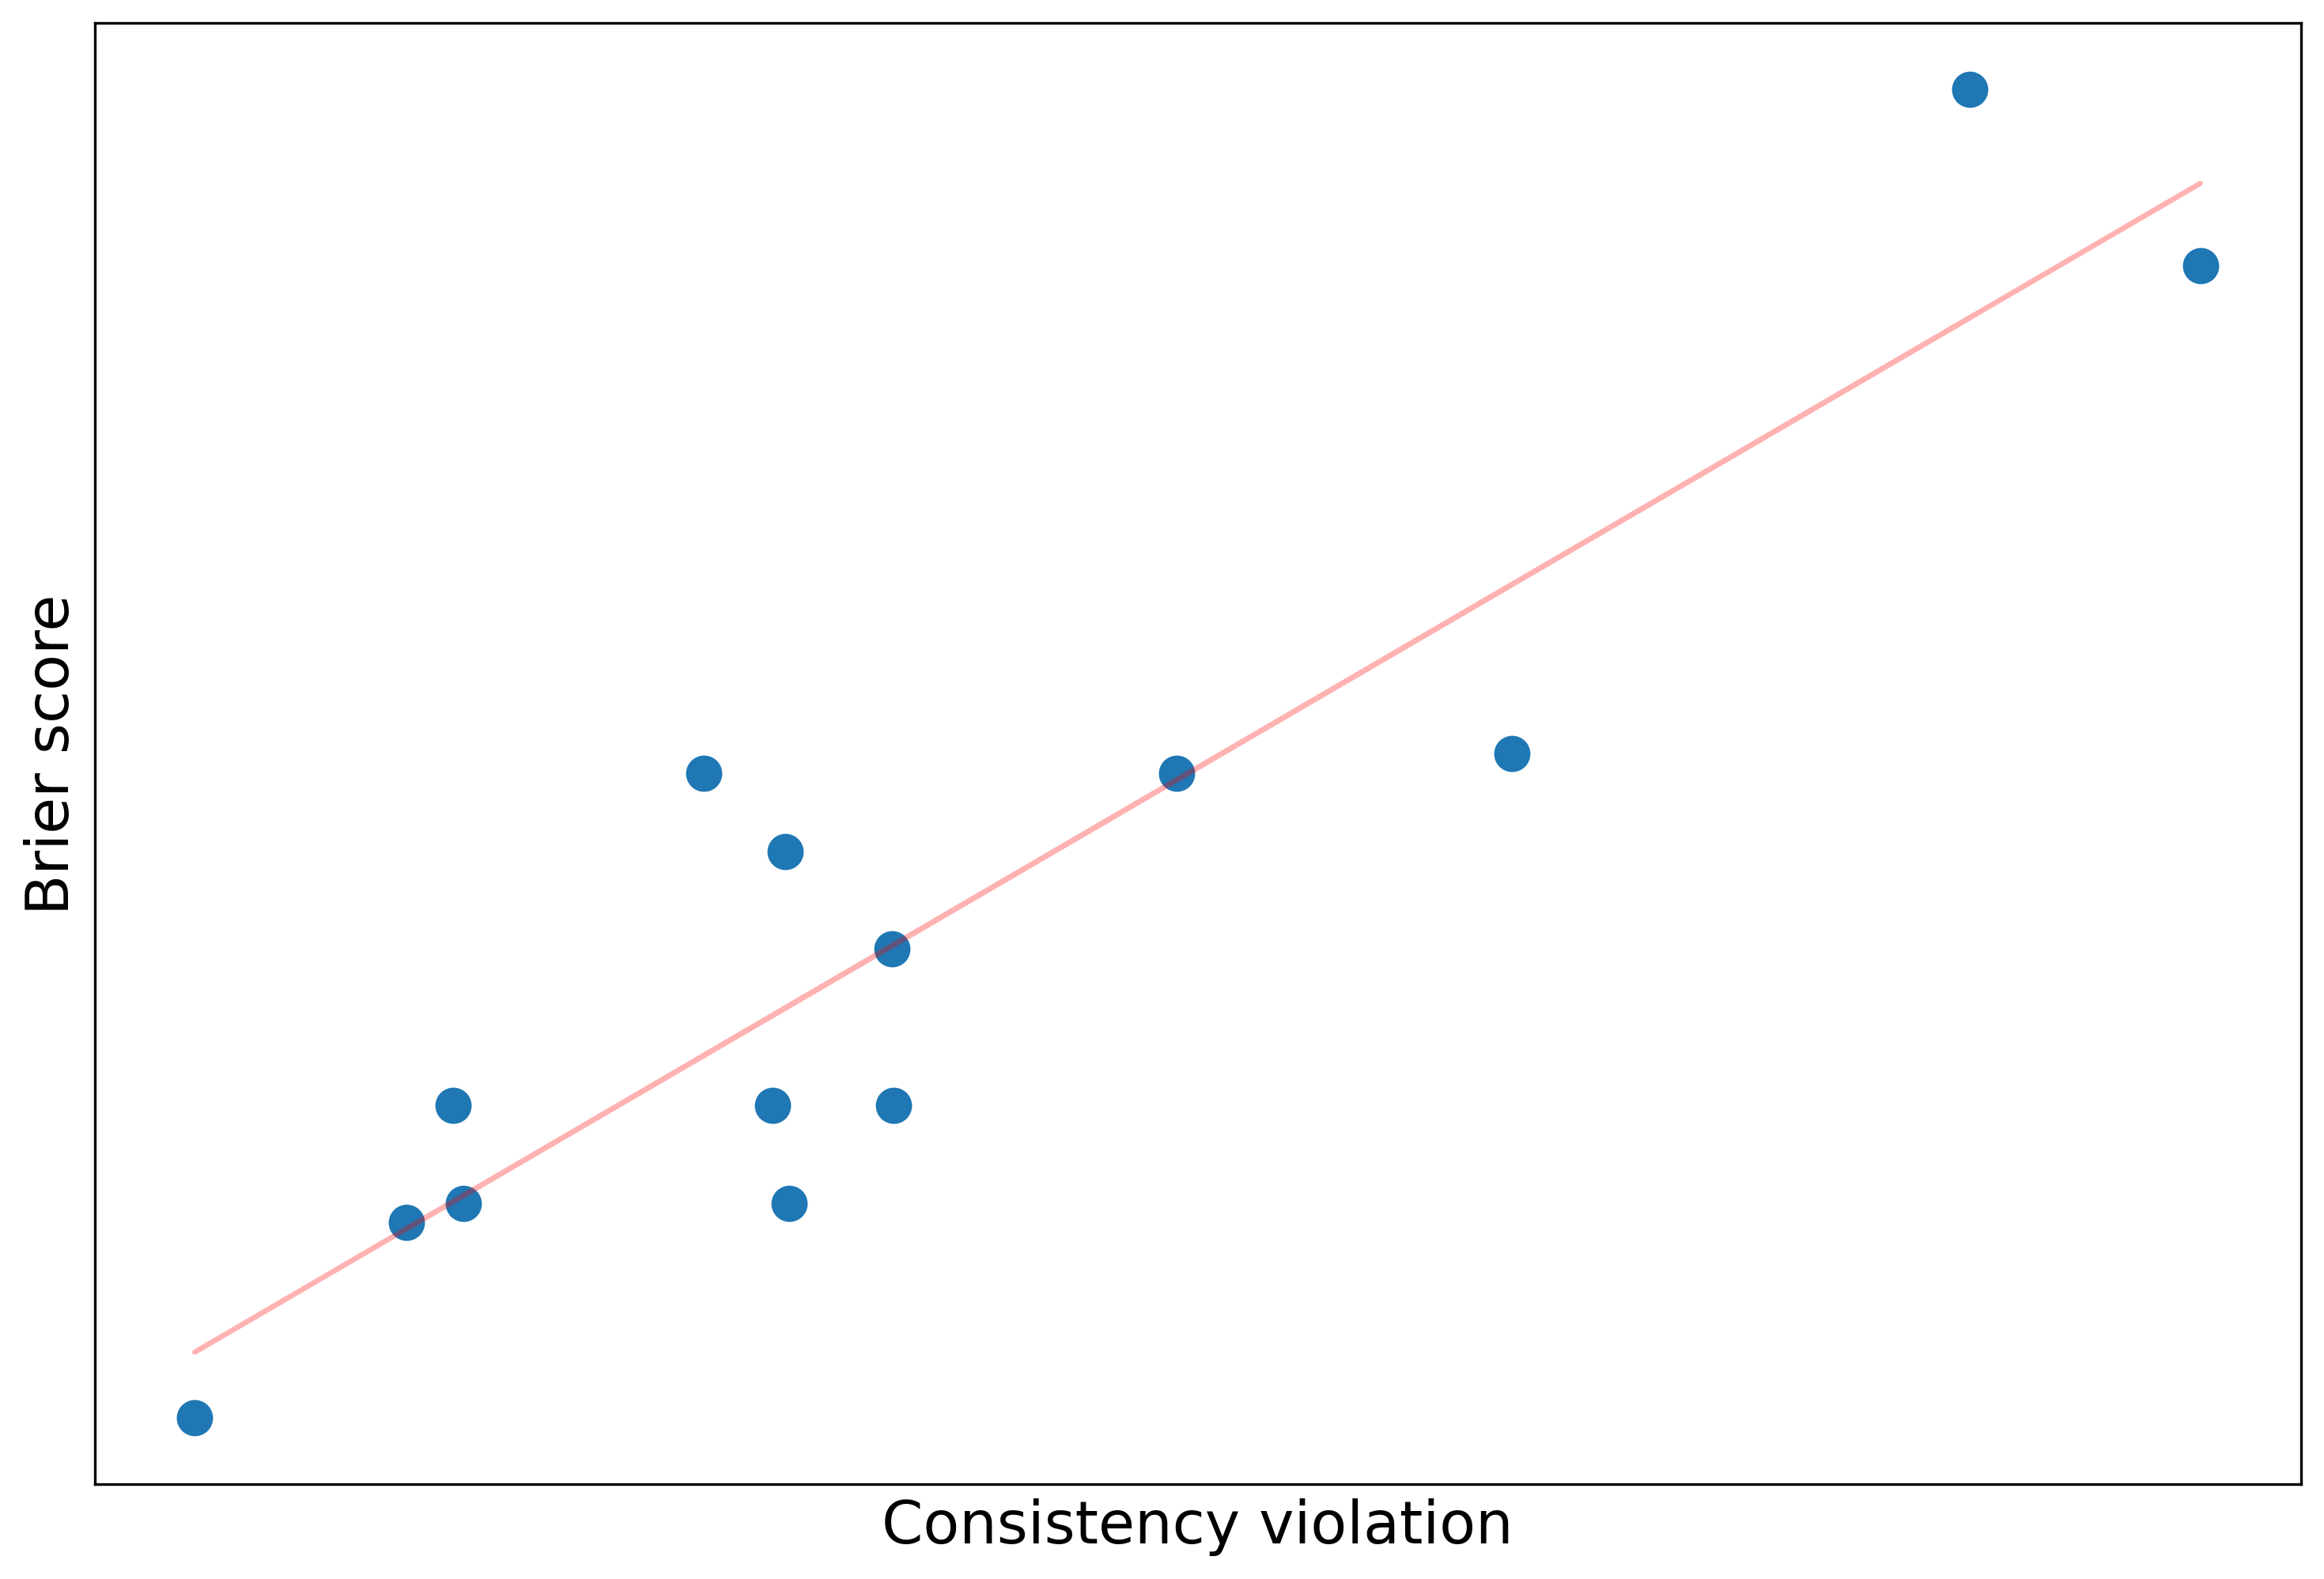
\includegraphics[width=\textwidth]{figures/consistency/CondChecker_vs_avg_brier_score_default_avg_violation_scraped_preview.png}
    \captionsetup{width=0.95\textwidth}
    \caption{
        The consistency violation scores on certain checks such as \CondChecker{} give signal about true forecasting performance over a range of forecasters, as described in \Cref{cfc/sec:results}.
    }
    \end{minipage}
    \label{fig:overview}
\end{figure}

\begin{table*}[hbtp]
\centering
\caption{Consistency checks used in our paper and the corresponding logical consistency conditions.}
\vspace{5pt}
\label{tab:consistency_checks}
\begin{tabular}{l p{0.65\linewidth}}
\toprule
\textbf{Name} &
\textbf{Condition ($\CCheck$)}
\\ \midrule
\NegChecker &
$\Forecaster(P)+\Forecaster(\lnot P)=1$
\\ \midrule
\begin{tabular}{@{}l@{}} \ParaphraseChecker\\ $\Relation(P,Q):=P\iff Q$\end{tabular} &
$\Forecaster(P)=\Forecaster(Q)$
\\ \midrule
\begin{tabular}{@{}l@{}} \ConsequenceChecker\\ $\Relation(P,Q):=P\implies Q$\end{tabular} &
$\Forecaster(P)\le\Forecaster(Q)$
\\ \midrule
\AndOrChecker &
$\Forecaster(P)+\Forecaster(Q)=\Forecaster(P\lor Q)+\Forecaster(P\land Q)$
\\ \midrule
\AndChecker &
$\max(\Forecaster(P)+\Forecaster(Q)-1, 0) \le \Forecaster(P\land Q) \le \min(\Forecaster(P),\Forecaster(Q))$
\\ \midrule
\OrChecker &
$\max(\Forecaster(P),\Forecaster(Q))\le\Forecaster(P\lor Q)\le\min(1,\Forecaster(P)+\Forecaster(Q))$
\\ \midrule
\ButChecker &
$\Forecaster(P\lor Q)=\Forecaster(P)+\Forecaster(\lnot P\land Q)$
\\ \midrule
\CondChecker &
$\Forecaster(P)\Forecaster(Q|P)=\Forecaster(P\land Q)$
\\ \midrule
\CondCondChecker &
$\Forecaster(P)\Forecaster(Q|P)\Forecaster(R|P\land Q) =\Forecaster(P\land Q\land R)$
\\ \midrule
\ExpectedEvidenceChecker &
$\Forecaster(P)=\Forecaster(P|Q)\Forecaster(Q)+\Forecaster(P|\lnot Q)(1-\Forecaster(Q))$
\\ \bottomrule
\end{tabular}
\end{table*}

%\include{tikzfig1}

Our contributions in this work are as follows:

\textbf{1) Principled metrics for consistency.~}
In \Cref{cfc/sec:background}, we introduce a theoretical framework for measuring consistency violations of binary forecasts, based on two metrics: an \emph{arbitrage metric}, based on market arbitrage, and a \emph{frequentist metric}, based on hypothesis testing. We apply these metrics to 10 different logical consistency rules (see \Cref{tab:consistency_checks}):
\NegChecker{}, \ParaphraseChecker{},  \ConsequenceChecker{}, \AndOrChecker{}, \AndChecker{}, \OrChecker{}, \ButChecker{}, \CondChecker{}, \CondCondChecker{} and \ExpectedEvidenceChecker{}.
%The metrics are introduced in \Cref{cfc/sec:consistency-checks-intro} and \Cref{cfc/app:arbitrage,cfc/app:frequentist-metric}.
%We leave training forecasters to be consistent with these metrics as an exciting direction for future work.

\textbf{2) A consistency evaluation pipeline for binary forecasters.~}
In \Cref{cfc/sec:pipeline}, we introduce a \emph{consistency evaluation pipeline} for LLM forecasters.
We create two forecasting datasets with known ground truth resolutions: one scraped from prediction markets, and one synthetically generated from news articles.
Both datasets include only events that happen past the training data cutoff of all forecasters we test, and resolve before September 2024.
We then generate tuples of forecasting questions satisfying logical consistency rules with associated consistency metrics.

%\evanunimp{keywords or categories/tags? -- I think keywords makes more sense in the intro (vin)}

\textbf{3) Consistency correlates with ground truth forecasting performance.}
Our consistency metrics are novel performance metrics for forecasters that can be computed right away, no matter the time horizon.
Of course, forecasters could also be evaluated using \emph{backtesting}, asking past questions with known ground truth resolutions.
Yet, backtesting LLM forecasters can be challenging if we do not have clear information about the models' training data contents. Moreover, there may be new types of questions that we want to evaluate forecasters on, for which we do not have appropriate past results (e.g., questions related to pandemics before 2020).
It is thus natural to ask:
\emph{can consistency metrics tell us anything about future forecasting performance?}

In \Cref{cfc/sec:results}, we show that for all forecasters we test, our consistency metrics correlate positively with forecasting performance (as measured by the Brier score) on both our benchmark datasets.
The correlation varies across consistency checks, with some logical checks (e.g., consistency of conditional probabilities) having over $R=0.9$ correlation with forecasting performance, while other logical tests provide little signal.
We \rebuttal{hypothesise that this analysis can extend} to smarter forecasters and longer time horizons, to provide instantaneous feedback on forecaster performance.

\textbf{4) Scaling inference-time compute can improve consistency for some logical checks, but fails to generalize.}
Since we find that consistency correlates with forecasting performance, it is natural to ask whether we can improve forecasters by making them more consistent. Unfortunately, we find that natural ways of improving consistency tend to overfit to specific consistency checks and do not generalize.

Specifically, we design \CFCaster{}: a forecaster that ``patches'' some base forecaster's output by generating logically related questions and ``arbitraging'' the base forecaster's forecasts for these related questions against each other.
In Section~\ref{cfc/sec:cfcaster} and \Cref{cfc/app:cfcaster}, we show that \CFCaster{} improves consistency on checks that we optimize against, but this improvement does not generalize to other held-out consistency checks, nor does it improve the actual forecasting performance.

\textbf{5) A long-horizon forecasting consistency benchmark.}
%In \Cref{cfc/sec:results} and \Cref{cfc/app:synthetic-questions-2028},
We create a long-horizon benchmark of 3,000 consistency checks for forecasts resolving in 2028. Our benchmark spans questions on various topics for which we will have no ground truth for more than three years, and thus serves as a nice testing ground for advanced LLM forecasters.


We release the full code \footnote{\url{https://github.com/dpaleka/consistency-forecasting}} and the datasets \footnote{\url{https://huggingface.co/datasets/dpaleka/ccflmf}} used in the paper.

%\towrite{list of experiments (list of forecasters tested, ground truth correlation, CF description, metaculus bot) -- or something.}

\section{A theoretical framework for forecasting consistency}
\label{cfc/sec:background}
\label{cfc/sec:forecasting}

%\section{Forecasting}
%\todo{I don't think there should be a subsection with just notation}

%\towrite{Background on Forecasting as a task @manyu.}

\begin{notation*}
    Let $\ForecastingQuestions$ denote the set of forecasting questions we are interested in, $\Resolutions$ denote the set of possible outcomes/resolutions for an individual questions.
    \rebuttal{
    In this paper, we focus on $\ForecastingQuestions$ as a set of binary forecasting questions, so $\Resolutions=\bools$.
    %and $\Forecasts=\probs$.
    }
    %and $\Forecasts$ denote the set of probability distributions on $\Resolutions$.
    A \emph{Forecaster} is then a map $\Forecaster:\ForecastingQuestions\to\probs$.
    One special forecaster is the ground truth resolutions $\Resolution:\ForecastingQuestions\to\Resolutions$, \rebuttal{returning $1$ and $0$ probability for $\bools$, respectively.}

    For conditional questions that can resolve to $\none$, we also have optional resolutions $\ResolutionsOpt:=\Resolutions\cup\{\none\}=\boolsopt$.
    We focus on binary questions following \cite{halawiApproachingHumanLevelForecasting2024}.
    \rebuttal{Our methods can in principle be extended to study consistency between general probability distributions in forecasting, such as the ones discussed in \citet{gooenScorableFunctionsFormat2024}.}
     %\manyuunimp{and because eliciting other probability distributions from LLMs is difficult (see the work of \citet{gooenScorableFunctionsFormat2024} for some work in this direction).}
     %i.e. Other questions types could involve a continuous value (what is the average temperate of New York in June 2025) or Multiple Choice (who will be the MVP of the NBA Championships in 2025?)  It is computationally intensive or intractable to test most consistency metrics with these types of questions.  However, multiple choice questions, can be subdivided into several binary questions, which is done in our set.  For example:  Will Lebron James by MVP in 2025; Will Kevin Durant be MVP in 2025...
\end{notation*}

\subsection{Consistency checks and inconsistency metrics}
\label{cfc/sec:consistency-checks-intro}

In line with \cite{esmwcc}, a consistency check is conceptualized as a pair of n-ary relations: \rebuttal{$\Relation:\ForecastingQuestions^n\to\bools$ in question space, $\CCheck:\probs^n\to\bools$ in forecast space, and a predicate for $\Forecaster$ such that $\Relation(x_1,\dots x_n)\implies\CCheck(\Forecaster(x_1), \dots \Forecaster(x_n))$.}
In particular, this assertion must be satisfied by all feasible $\Resolution$, and also any ``correct'' forecasts generated by a world model that accurately accounts for aleatoric uncertainty.
Violation of consistency is measured by some violation metric $\Violation:\probs^n\to\Reals$ which must satisfy $\Violation(\Forecaster(x_1),\dots\Forecaster(x_n))=0\iff\CCheck(\Forecaster(x_1),\dots\Forecaster(x_n))$.
%
For example, intuitively, the ``negation'' check \NegChecker{} is given by \rebuttal{the relation $\Relation(x_1,x_2) := x_1=\lnot x_2$ on questions, and the relation $\CCheck(\Forecaster(x_1), \Forecaster(x_2)) := \Forecaster(x_1)+\Forecaster(x_2) \approx 1$ on forecasts.}
The full table of the consistency checks we use is given in Appendix~\ref{cfc/app:checks}.

Improving upon \cite{esmwcc}, we derive $\Violation$
%(and therefore $\CCheck$)
from $\Relation$ in a principled way,
handling all types of logical consistency checks simultaneously.
We introduce two new \emph{inconsistency metrics}: the \emph{arbitrage metric} and the \emph{frequentist metric} for measuring logical inconsistency in probabilistic forecasts.

\subsubsubsection{Arbitrage metric}
\label{cfc/sec:arbitrage}

\NewDocumentCommand{\score}{m}{\ensuremath{s\left(#1\right)}}
\NewDocumentCommand{\consp}{}{p}
\NewDocumentCommand{\argmaxmax}{}{\mathop{(\argmax,\max)}}

The arbitrage metric is conceptualized as the minimum profit that an arbitrageur can be guaranteed making bets against the forecaster's predictions. More precisely: suppose that the forecaster's probabilities $\Forecaster(x_1),\dots\Forecaster(x_n)$ were prices offered by a logarithmic market maker \footnote{
A \emph{logarithmic market maker} with subsidy $w$ is a market maker who adjusts prices in response to trades such that the trader's reward for moving the probability of a true-resolving sentence from $p_0$ to $p'$ is $w\log p'-w\log p_0$.
%\rebuttaldeleted{Manifold Markets uses such a procedure.}
For further background on scoring rules and the associated market makers, see Appendix~\ref{cfc/app:arbitrage}, \rebuttal{\cite{berg2009hanson},}
or \cite{hansonLogarithmicMarketScoring2002}.
}  with market subsidy parameter \$1.
If these probabilities are inconsistent, then there are prices $p_1,\dots p_n$ that an arbitrageur could bring to the market such that it is guaranteed to make a profit against the market-maker, no matter the outcome of each question. We \rebuttal{define} $\Violation(\Forecaster(x_1),\dots\Forecaster(x_n))$ \rebuttal{as the maximum achievable} ``minimum profit'' that the arbitrageur can guarantee by choosing appropriate $p_1,\dots p_n$. We further denote by $\Arbitrageur(\Forecaster(x_1),\dots\Forecaster(x_n))$ the set of prices $p_1,\dots p_n$ that maximize the minimum profit:
\ft{math is hard to parse, just rewrite}
%This can also be interpreted as the ``minimum number of bits of information lost to inconsistency''.
%
\begin{equation}
\resizebox{.95\hsize}{!}{$\displaystyle
    \argmaxmax_{\consp\in[0,1]^n} \min_{\omega\in\Omega} \sum_{i=1}^n \left(\log{\consp_i}-\log{\Forecaster(x_i)}\right)\Indicator{\omega(i)=\top} + \left(\log{(1-\consp_i)}-\log{(1-\Forecaster(x_i))}\right)\Indicator{\omega(i)=\bot}$}
    \label{eq:arbitrage__}
\end{equation}
%
Here $\Omega:=\{\omega\in\ResolutionsOpt^n\mid\Relation(\omega)\}$ is the set of all possible consistent resolutions of this tuple. A more general version of ~\ref{eq:arbitrage__} is given in Appendix~\ref{cfc/app:arbitrage}, along with specific worked-out examples of the arbitrage metric for each consistency check, and details on how we compute it; as an example, the arbitrage metric for the Negation Check can be derived exactly (Appendix~\ref{apps:arbitrage-neg}):
%
\begin{equation*}
\begin{split}
    \Violation(\Forecaster(x),\Forecaster(\lnot x))=-2\log\left(\sqrt{\Forecaster(x)(1-\Forecaster(\lnot x))}+\sqrt{(1-\Forecaster(x))\Forecaster(\lnot x)}\right)
\end{split}
\end{equation*}
%
% \begin{definition}[Arbitrage-based Violation Metric]
%     Let $\Relation:\ForecastingQuestions^n\to\bools$ be an n-ary relation such that $\Relation(\Resolution(x_1), \dots \Resolution(x_n))$ is satisfied by the ground-truth resolutions $\Resolution:\ForecastingQuestions\to\Resolutions$ for all tuples $(x_1,\dots x_n)$. \footnote{This is well-defined because resolutions can be taken as a subset $\Resolutions\subseteq\ForecastingQuestions$, by treating them as forecasting questions that always resolve to themselves by definition. For example, the forecasting question $\top$ is always worth \$1 and the forecasting question $\bot$ is always worth \$0.} Let $s:\ForecastingQuestions\times\Resolutions\times[0,1]\to\Reals$ be a proper scoring rule that gives the score earned based on the probability assigned to the true resolution, e.g. $s(x,\Resolution,p(\Resolution))=\log p(\Resolution)$. Let $(x_1,\dots x_n)\in\ForecastingQuestions^n$ be a question tuple, and denote $\ResolutionsVec:=\{\resolutionvec\in\ResolutionsOpt^n\mid\Relation(\resolutionvec)\}$ the set of possible consistent resolutions (including $\none$ resolutions) of this tuple. Then for forecasts $(\Forecaster(x_1),\dots\Forecaster(x_n))$ the arbitraged forecasts $\Arbitrageur(\Forecaster(x_1),\dots\Forecaster(x_n))=(p_1\dots p_n)$ and the minimum guaranteed profit of the arbitrageur $\Violation(\Forecaster(x_1),\dots\Forecaster(x_n))$ are given by:
%
%     \begin{equation}
%         \argmaxmax_{\consp\in\Forecasts^n}
%         \min_{\resolutionvec\in\ResolutionsVec}
%         \sum_{i=1}^n
%         %\sum_{\Resolution\in\Resolutions}
%         \score{x_i, \resolutionvec_i, p_i(\resolutionvec_i)}
%         - \score{x_i, \resolutionvec_i, \Forecaster(x_i)(\resolutionvec_i)}%\Indicator{\omega_i=\Resolution}
%         \label{eq:arbitrage}
%     \end{equation}
%     Where by convention, any score on a resolution $\resolutionvec_i=\none$ is taken to be 0.
%     \label{def:arbitrage}
% \end{definition}
%
% Definition~\ref{def:arbitrage} is presented in full generality: $\consp$ and $\Forecaster(x_i)$ here are \emph{probability distributions} on $\Resolutions$. Breaking it down: each $\score{x_i, \resolutionvec_i, p_i(\resolutionvec_i)}- \score{x_i, \resolutionvec_i, \Forecaster(x_i)(\resolutionvec_i)}$ gives the arbitrageur's profit on the market for question $x_i$, given that it resolves $\resolutionvec_i$. The profit is summed across all markets in the tuple, and then minimized over all consistent worlds; this minimum is maximized across all possible arbitrageur bets.
%
% It is helpful to explicitly state Eq~\ref{eq:arbitrage} in the case of binary forecasting questions, as follows.
%
% \begin{equation}
%     \argmaxmax_{\consp\in[0,1]^n} \min_{\omega\in\Omega} \sum_{i=1}^n \left(\score{\consp_i}-\score{\Forecaster(x_i)}\right)\Indicator{\omega(i)=\top} + \left(\score{1-\consp_i}-\score{1-\Forecaster(x_i)}\right)\Indicator{\omega(i)=\bot}
%     \label{eq:arbitrage_}
% \end{equation}

% Appendix~\ref{cfc/app:arbitrage} includes specific worked-out examples of the arbitrage metric for each consistency check, and details on how we compute it; as an example, the arbitrage metric for the Negation Check can be derived exactly (Appendix~\ref{apps:arbitrage-neg}):


To illustrate: $\Violation(0.5,0.6)\approx 0.01$, $\Violation(0.5,0.51)\approx 10^{-4}$.
The metric is more sensitive to violations for probabilities very close to $0$ or $1$, due to the logarithmic market maker.
% TODO examples of this here
In our evals, for all types of checks, we say that a sampled check does not pass if $\Violation \ge 0.01$.
\rebuttal{We have to pick some hyperparameter as an inconsistency threshold; we set it to correspond} to
giving 110\% probability in total to the events of Republican and Democratic parties winning the US presidential election.

\subsubsubsection{Frequentist metric}
\label{subcfc/sec:frequentist-metric}

We also compute a different, \emph{frequentist} consistency metric. Consider a Monte Carlo forecaster that samples a world model $n$ times, and for any event, returns the fraction of samples in which the event occurs. The frequentist metric is the number of standard deviations a given tuple forecast is off from the mean Monte Carlo forecast, scaled to be independent of $n$. We say that a consistency violation happened if the number of standard deviations away from the mean of the null is at least as in the $(0.5, 0.6)$ case described in \Cref{cfc/sec:arbitrage}. The full description is given in \Cref{cfc/app:frequentist-metric}.
%\adamunimp{we should say what we picked as sigma = 0.05 here?}.\dpaleka{no,wit's confusing enough as it is}


\subsubsubsection{Intuition on consistency metrics}

Our metrics address two major obstacle with measuring inconsistency: \emph{tolerance to noise} and \emph{principled aggregation of inconsistency scores}.

\textbf{Tolerance to noise.}
In the standard Bayesian setting, beliefs are either consistent or not: there either is a Dutch book (a way to bet against the forecaster's beliefs to get infinite profit) or the probabilities are perfectly consistent.
In practice, an forecaster's beliefs (even on the same question) are never perfectly consistent across runs. If an election model has a presidential candidate at 48\% with one random seed and 50\% on the other, this is not a reason to discard it as completely flawed. Hence, instead of a binary measure of consistency, our metrics increase smoothly with inconsistency.

\textbf{Principled aggregation and comparison of inconsistency scores.}
\cite{esmwcc} developed a set of inconsistency checks, used an ad-hoc metric for each check they used, and normalized the scores to [0, 1].
There are two major issues with their approach:
\begin{enumerate}
    \item The metrics in their work are mostly \emph{linear} and would treat the inconsistencies of $(0.5, 0.6)$ and $(0.89, 0.01)$ on the $\NegChecker$ check the same, which is counter-intuitive in many applications.
    \item It is unclear how to compare and aggregate scores from different consistency checks.
\end{enumerate}
Our approach ensures that all consistency scores share a common ``unit''. For example, in the arbitrage metric, to aggregate inconsistencies, we sum up the profit made by an arbitrageur across questions.


\section{Pipeline overview}
\label{cfc/sec:pipeline}
%\manyuunimp{is it better to just title as Methods?}

We illustrate the steps in our data collection pipeline below, and provide more details on each individual steps:
%
\begin{equation*}
    \fbox{\text{\small\emph{Online platforms, news, topics}}}\ \xrightarrow[\text{+scraping}]{\text{synthetic}}\ P\ \xrightarrow[\text{instantiation}]{\text{tuple}}\ (P,Q)\ \xrightarrow{\Forecaster}\ (p,q)\ \xrightarrow{\Violation}\ \Violation(p,q)
\end{equation*}

\begin{itemize}
    \item ($\dots\longrightarrow P$) We first prepare datasets of \textbf{base questions} in multiple ways:
    \begin{enumerate}[label=(\alph*)]
        \item Scraping questions from online platforms such as Manifold and Metaculus;
        \item A ground-truth resolved dataset synthetically generated from news articles;
        \item Synthetic generation on questions on a list of topics such as Politics, Science, Economics, etc.
    \end{enumerate}
    For the first two of the above, we also include the \emph{ground truth resolution} for each question.
    % We discuss all of these in more detail in \Cref{cfc/sec:fq-generation}.
    %\item ($\dots\longrightarrow P$) A dataset of \textbf{base questions} is prepared from a combination of \emph{(a)} scraping from online platforms such as Manifold and Metaculus and \emph{(b)} synthetic generation. % Steps are taken to ensure sufficient diversity of questions in the dataset to avoid biasing towards a particular topic or style of question.
    \item ($P\longrightarrow (P, Q)$) The base questions are synthetically \textbf{instantiated into tuples} that must satisfy certain consistency checks. For example, every single base question $P$ is instantiated into a tuple $(P,\lnot P)$; and pairs of mutually relevant base questions $P,Q$ are instantiated into tuples like $(P,Q,P\land Q,P\lor Q)$. % Steps are taken to ensure the relevance of chosen base questions to each other (i.e. so that $P,Q$ are not ``Will our paper receive at least 100 citations?'' and ``Will it rain in Singapore on Christmas eve?'')
    \item ($(P,Q)\xrightarrow{\Forecaster}(p,q)$) The forecaster is separately queried to elicit \textbf{forecasts} on each question, resulting in forecast tuples that should, if the forecaster is consistent, satisfy consistency properties.  For example, for a size-two tuple where $Q = \neg P$, it should satisfy $p+q=1$.
    %\Alejandro{The term base question above is used to refer to the questions before making the tuples. The forecaster is queired on all of the questions in the tuple, not just the base question}
    \item ($(p,q)\xrightarrow{\Violation}\Violation(p,q)$) We score each tuple of forecasts for consistency with both of our violation metrics.
\end{itemize}

% maybe add a figure (pipeline.tex after some cleanup) -- or just this:

% A brief description of our overall pipeline for generating and evaluating consistency checks on forecasters:\todo{vin: done, but give it a read again. change P,Q to $x_1$, $x_2$ to maintain consistency throughout document}

% \begin{itemize}
%     \item ($\dots\longrightarrow x_i$) We prepare datasets of \textbf{base questions} in multiple ways:
%     \begin{enumerate}[label=(\alph*)]
%         \item Scraping questions from online platforms such as Manifold and Metaculus;
%         \item A ground-truth resolved dataset synthetically generated from news articles;
%         \item Synthetic generation on questions on a list of topics such as Politics, Science, Economics, etc.
%     \end{enumerate}
%     For the first two of the above, it is important to note that we also include the \emph{ground truth resolution} for each question.
%     We discuss all of these in more detail in \Cref{cfc/sec:fq-generation}.
%     %\item ($\dots\longrightarrow P$) A dataset of \textbf{base questions} is prepared from a combination of \emph{(a)} scraping from online platforms such as Manifold and Metaculus and \emph{(b)} synthetic generation. % Steps are taken to ensure sufficient diversity of questions in the dataset to avoid biasing towards a particular topic or style of question.
%     \item ($x_i\longrightarrow (x_i, x_j)$) The base questions are synthetically \textbf{instantiated into tuples} that must satisfy certain consistency checks. E.g. every single base question $x_i$ is instantiated into a tuple $(x_i,\lnot x_i)$; pairs of separate base questions $x_i,x_j$ are instantiated into tuples like $(x_i,x_j,x_i\land x_j,x_i\lor x_j)$. % Steps are taken to ensure the relevance of chosen base questions to each other (i.e. so that $P,Q$ are not ``Will our paper receive at least 100 citations?'' and ``Will it rain in Singapore on Christmas eve?'')
%     \item ($(x_i,x_j)\xrightarrow{\Forecaster}(\Forecaster(x_i),\Forecaster(x_j))$) The forecaster is \textbf{separately} queried to elicit \textbf{forecasts} on each question, resulting in forecast tuples that should, if the forecaster is consistent, satisfy consistency properties.  For example, in the case of $x_i = \neg x_j$, it should satisfy $\Forecaster(x_i)+\Forecaster(x_j)=1$.
% %    \Alejandro{The term base question above is used to refer to the questions before making the tuples. The forecaster is queried on all of the questions in the tuple, not just the base question}
%     \item ($(\Forecaster(x_i),\Forecaster(x_j))\xrightarrow{\Violation}\Violation(\Forecaster(x_i),\Forecaster(x_j))$) We score each tuple of forecasts for consistency with our violation metric.
% \end{itemize}

% % maybe add a figure (pipeline.tex after some cleanup) -- or just this:
% \begin{equation*}
%     \dots\xrightarrow[\text{+scraping}]{\text{synthetic}} x_i \xrightarrow[\text{instantiation}]{\text{synthetic}} (x_i,x_j) \xrightarrow{\Forecaster}\Forecaster(x_i),\Forecaster(x_j)\xrightarrow{\Violation}\Violation(\Forecaster(x_i),\Forecaster(x_j))
% \end{equation*}

% %Some details for each step are given below.
% Examples of data at each step of the pipeline are given in Appendix~\ref{cfc/app:details-dt}. The prompts and LLM calls used in each step before forecasting are given in Appendix~\ref{cfc/app:details-prompt}.

% \section{Generating and scraping forecasting questions}
% \label{cfc/sec:fq-generation}
% % \vin{Add details on when do questions resolve in all of these, see README.md}

% %\paragraph{Forecasting question format} Previous research on forecasting questions often overlooks critical details, such as thorough resolution criteria and precise resolution dates (e.g., \cite{zou2022forecasting} relies on short question titles for predictions). In contrast, our approach offers a more comprehensive specification, pairing a concise title with an extended body that clarifies and disambiguates the resolution criteria, along with relevant metadata. A full description of the data format is provided in Appendix \ref{cfc/app:details-fq-datatype} % Additionally, we include essential fields such as the precise resolution date, question creation date, and relevant metadata, ensuring clarity and robustness in the forecasting process.
% \paragraph{Forecasting question format.}
% Each forecasting question includes a title that states the main question, a body that provides detailed resolution criteria, and a resolution date, along with optional fields such as metadata and creation date.
% %For more, see \Cref{cfc/app:details-fq-datatype}.

% % \vin{describe what it is, reference the relevant appendix section, update it, move it to the first sec of the appendix, be brief here}


% \paragraph{Real prediction market questions.}
% We scrape questions from two forecasting platforms, Metaculus and Manifold Markets, and only use questions that both resolved and were initially set to resolve between May 1, 2024, and August 15, 2024.
% This leaves us with over 500 questions, of which 242 pass our verification step (see end of this subsection).
% An example of a processed question, including its relevant details, is provided in Appendix \ref{cfc/app:details-fq-datatype}.

% %\paragraph{Generating forecasting questions from NewsAPI articles}
% %We generate forecasting questions by filtering a curated selection of news articles sourced from NewsAPI\footnote{https://newsapi.org/}, with a particular emphasis on articles that describe concrete phenomena rather than opinion pieces. This approach ensures that our questions are rooted in factual events.
% %To mitigate subtle biases towards a particular resolution, we create additional questions using reference class spanning: using an LLM to modify entities and locations within the questions to diversify the range of scenarios.
% %Each question's ground-truth resolution is verified using the Perplexity API, yielding ground truth resolution labels with less than 5\% error rate in our testing.
% %From this process, we compile a dataset of 2,621 ground-truth resolved forecasting questions resolving between July 1, 2024, and August 31, 2024, inclusive.
% %We test the ground truth questions using a subset of 1,000 forecasting questions for our experiments.
% %The full dataset serves to instantiate 3,000 consistency check tuples in our pipeline.
% %Further details regarding the pipeline can be found in Appendix \ref{cfc/app:gen-fq-from-news}.

% \paragraph{Generating forecasting questions from NewsAPI articles.}
% To generate forecasting questions with known resolutions, we use articles sourced from NewsAPI\footnote{https://newsapi.org/}. We focus on articles describing concrete events rather than opinion pieces. To mitigate biases towards positive resolutions (as most questions derived from an article would typically resolve to True), we employ reference class spanning - using an LLM to modify key entities in the questions while keeping the overall thematic structure intact. Each question's ground-truth resolution is verified using the Perplexity API with internet access, yielding ground truth resolution labels with less than a 5\% error rate in our testing. We compile a total of 2,621 ground-truth resolved forecasting questions resolving between July 1, 2024, and August 21, 2024. Of these, we use a subset of 1,000 to test the relationship between consistency violation and accuracy.
% Further details regarding the pipeline can be found in Appendix \ref{cfc/app:gen-fq-from-news}.

% %\paragraph{Synthetic question generation}
% %We generate questions by few-shot prompting, starting from a handpicked set of a few question titles for several topics.
% %Once a question is verified to be valid, we add it to our question database, and reuse it in few-shot prompting for new questions.
% %To get a more diverse set of questions, we additionally deduplicate the question database based on a similarity threshold on the \textembedsmall{} embeddings from OpenAI.
% % \Alejandro{Comment: With the last changes titles, bodies and dates are generated simultaneously. Should we add the use of tags for getting diverse questions?} Once the titles are generated, we create question bodies and resolution dates using a few-shot prompt to \gptfouro{}, resulting in 1,000 forecasting questions that resolve either by or in 2028. More details are in \Cref{cfc/app:details-prompt}.

% \paragraph{Synthetic question generation.}
% We generate questions by few-shot prompting, we sample six examples of forecasting questions, as style examples, as well as a set of tags (Brazil, NBA...) to diversify the generated questions.
% We generate question titles, deduplicate them using \textembedsmall{} embeddings from OpenAI, and then for each title we use \gptfouro{} to create the question body and resolution date. With this method we create 1,000 forecasting questions that resolve either by or in 2028. More details are in \Cref{cfc/app:details-prompt}.


% \paragraph{Verification and improvement from human feedback.}
% In all of the above steps, we filter generated questions in using \gptfouro{} to check for properties such as the coherence between the body and title, the clarity and precision of the resolution criteria, and whether the question is about actual world events.
% Questions failing this step are discarded.
% To develop this step, we used a feedback form for human reviewers (authors of this paper) to suggest modifications to generated questions. These suggestions inform refinements to prompts and few-shot examples in our pipeline. An example of the feedback form is provided in Appendix \ref{cfc/app:feedback_form}.

% \section{Instantiating tuples of questions for consistency checks}
% \label{cfc/sec:instantiation}

% The base forecasting questions are subsequently used to synthetically generate tuples of logically related questions. For example, a pair of base questions $(P,Q)$ can be used to generate a 4-tuple $(P,Q,P\land Q,P\lor Q)$ for \AndOrChecker{}, or a 3-tuple $(P,\lnot P\land Q, P\lor Q)$ for \ButChecker{} (see Appendix~\ref{cfc/app:checks} for details). The main question content (titles and bodies) were generated synthetically (using \texttt{gpt-4o}), while the resolution dates and other properties were calculated systematically (e.g. the $\max$ of the resolution dates of the base questions).

% We then conduct two measures to ensure the instantiated tuples are correct and \rebuttal{sensible}: relevance scoring, and verification that the tuples of questions indeed describe logically related events.

% \paragraph{Relevance scoring.}
% When combining base questions into tuples, we have to take care to avoid off-distribution questions like ``Is SpaceX going to be worth \$200B by 2030, given that Sri Lanka's rice production grows 40\% by 2040?''.
% For tuples instantiated from more than one base question, we sort 2000 potential base question combinations by their ``relevance score'', obtained by querying an LLM and asking it to score how relevant the questions are to one another, and choose the top 200 for each consistency check. See \Cref{fig:relevance-prompt} for details.

% %\todo{Adam: not sure if talking about a discriminator is necesarry?  Also we never really define what good enough results are}
% %Another approach would be to finetune a discriminator to verify questions in the instantiated tuple are within the distribution of real forecasting questions; however, the simple LLM relevance scoring gives sufficiently good results. In Appendix~\ref{cfc/app:details-dt}, we show an example of a tuple instantiated from well-selected base questions.
% %
% %\todo{Adam:  this last paragraph on all checks except consequence isn't very clear...For this check only, we generated 100 tuples and manually filtered to 50/30 tuples which clearly encode a logical implication, both in the title and body fields.}

% \paragraph{Verification.}
% The instantiated tuples of questions are then passed to another LLM call to reject if they do not fit their intended structure; for example, we detect if the resolution criteria of the second question are not truly a negation of the resolution criteria of the first question.
% Examples of verification prompts are given in \Cref{cfc/app:details-prompt}.
% %We additionally inspect and filter a sample of instantiated tuples manually.
% %To improve performance and aid oversight, the LLM was asked to provide chain-of-thought reasoning \cite{weiChainofThoughtPromptingElicits2022} for accepting or rejecting a given tuple.
% %For all checks except \ConsequenceChecker, manual filtering did not remove any ambiguous or wrongly instantiated tuples; we conclude the failure rate of our instantiation is less than 5\% on our base question distribution.
% %For \ConsequenceChecker, even after verification, our instantiation still produces ambiguous or invalid tuples over 30\% of the time.
% %For this check only, we generate 100 tuples from each of the scraped synthetic base question, and manually filter to 50/30 valid tuples.
% %which clearly encode a logical implication, both in the \emph{title} and \emph{body} fields.

% \section{Eliciting forecasts}

% We test a range of forecasters based on various LLM models (\gptfouro{}, \gptfouromini{}, \claudesonnet{}, \llamaeight{}, \llamaseventy{}, \llamafourhundred{}, \oonemini{} and \oonepreview{}) with and without chain-of-thought prompting: see \Cref{cfc/app:forecasters} for details.
% We run each of these forecasters on 5000 tuples in total (for each of the 10 checks, we use 200 tuples from scraped questions and 300 from NewsAPI questions), except for \oonepreview{}, which we test on 50 tuples per check only due to cost constraints.
% We could not test forecasters from \cite{halawiApproachingHumanLevelForecasting2024} due to API deprecations; see \Cref{cfc/sec:cannot_evaluate_halawi}.



\section{Results}
\label{cfc/sec:results}

We evaluate a range of forecasters on the datasets described above, for both consistency and ground truth Brier score.
We note that the Brier score as the standard metric of forecasting accuracy depends both on model capabilities and the training data cutoff: it should not be surprising for a stronger model to have a worse Brier score if its training data cutoff is earlier than for a weaker model.
% The full list of forecasters is in \Cref{cfc/app:forecasters}.

For all data analysis in this section, we exclude forecasters that have Brier score worse than random guessing (0.25), such as the basic setup with \llamaeight{}, as it would unfairly advantage our case of ``correlating consistency with accuracy''.



\textbf{Average consistency scores correlate \rebuttal{strongly} with forecasting performance.}
We can aggregate the consistency scores across all checks for each forecaster \rebuttal{
by aggregating either the arbitrage or the frequentist violations.}

%\rebuttalremoved{
%For aggregate metrics, we scale the  arbitrage violations by the reciprocal of the number of questions in a tuple, due to the market liquidity intepretation in \Cref{cfc/app:arbitrage}.
%}


We plot the average Brier score against the three aggregate consistency scores in \Cref{fig:consistency_vs_brier}.

\begin{figure}[h]
    \centering
    \begin{subfigure}[b]{0.48\textwidth}
        \centering
        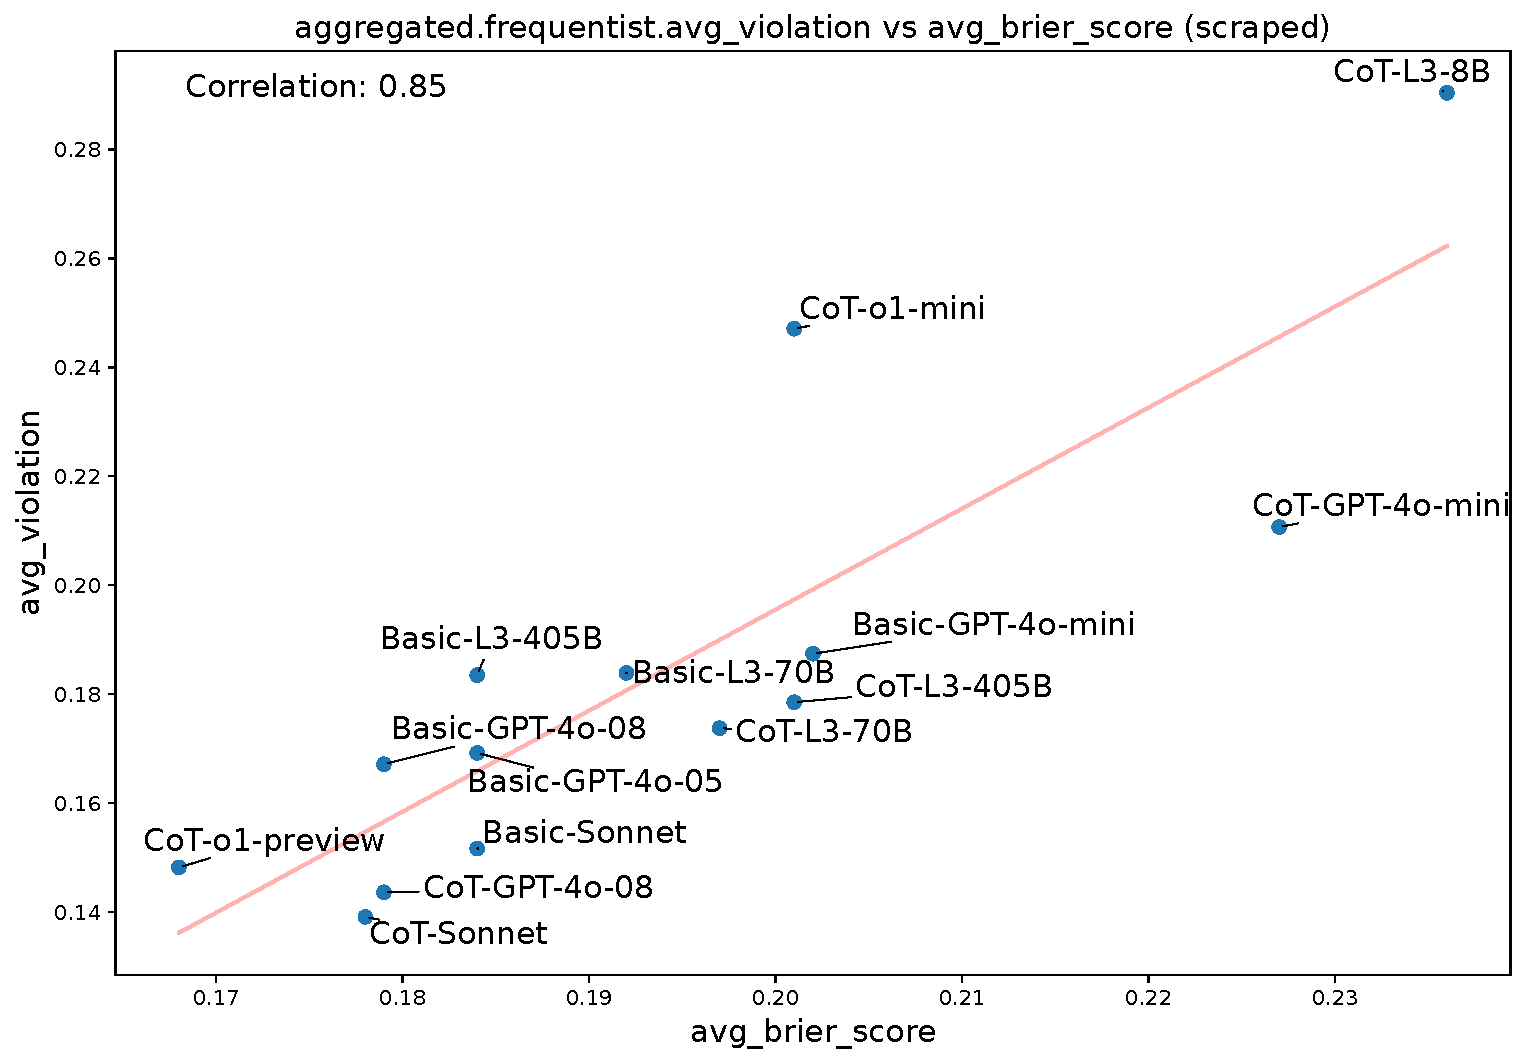
\includegraphics[width=\textwidth]{figures/consistency/aggregated_vs_avg_brier_score_frequentist_avg_violation_scraped.pdf}
        \caption{
         Aggregate frequentist metric on the scraped forecasting question dataset.
        }
        \label{fig:aggregate_vs_avg_brier_frequentist_scraped}
    \end{subfigure}
    \hfill
    \begin{subfigure}[b]{0.48\textwidth}
        \centering
        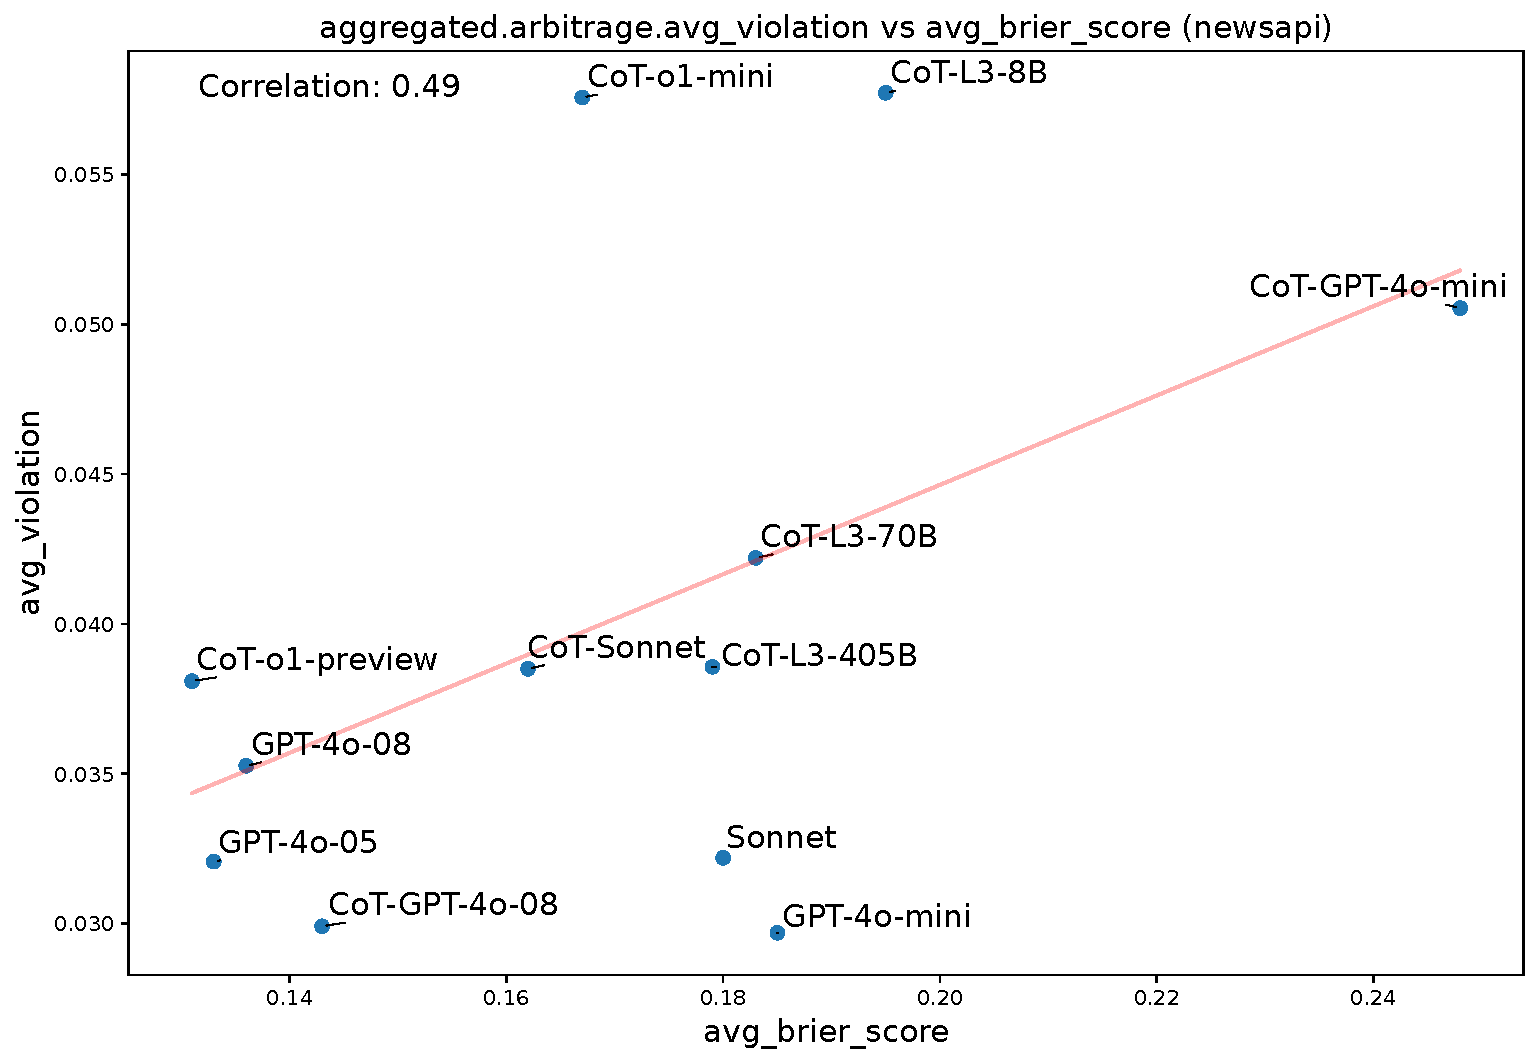
\includegraphics[width=\textwidth]{figures/consistency/aggregated_vs_avg_brier_score_default_avg_violation_newsapi.pdf}
        \caption{
         Aggregate arbitrage metric on the NewsAPI questions dataset.
        }
        \label{fig:aggregate_vs_avg_brier_arbitrage_newsapi}
    \end{subfigure}
    \caption{
        Scatter plots showing the relationship between consistency metrics and average Brier scores for different forecasters.
        Each point represents a forecaster, with the x-axis showing the average Brier score and the y-axis showing the consistency metric .
        The y-axis values are aggregated across all checks for each forecaster and averaged over the instantiated consistency check tuples.
        Lower scores are better for both axes.
    }
    \label{fig:consistency_vs_brier}
\end{figure}


\begin{figure}[h]
    \centering
    \begin{subfigure}[b]{0.48\textwidth}
        \centering
        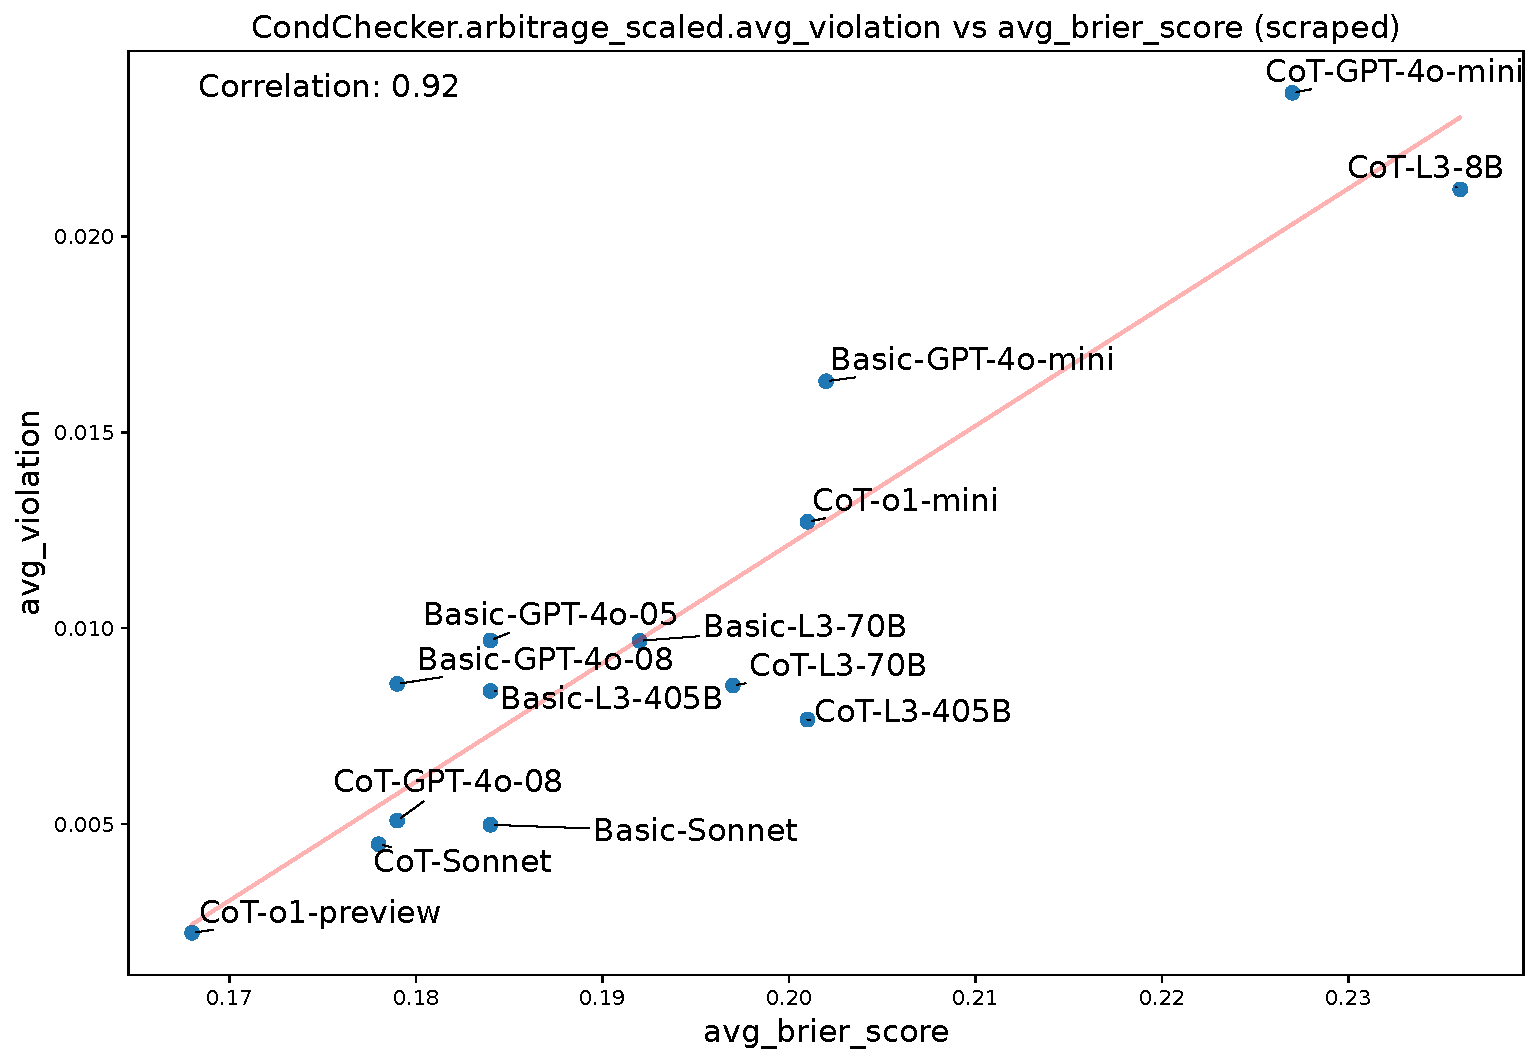
\includegraphics[width=\textwidth]{figures/consistency/CondChecker_vs_avg_brier_score_default_scaled_avg_violation_scraped.pdf}
        \caption{
         \CondChecker{} arbitrage metric on the scraped forecasting question dataset.
        }
        \label{fig:condchecker_vs_brier_scraped}
    \end{subfigure}
    \hfill
    \begin{subfigure}[b]{0.48\textwidth}
        \centering
        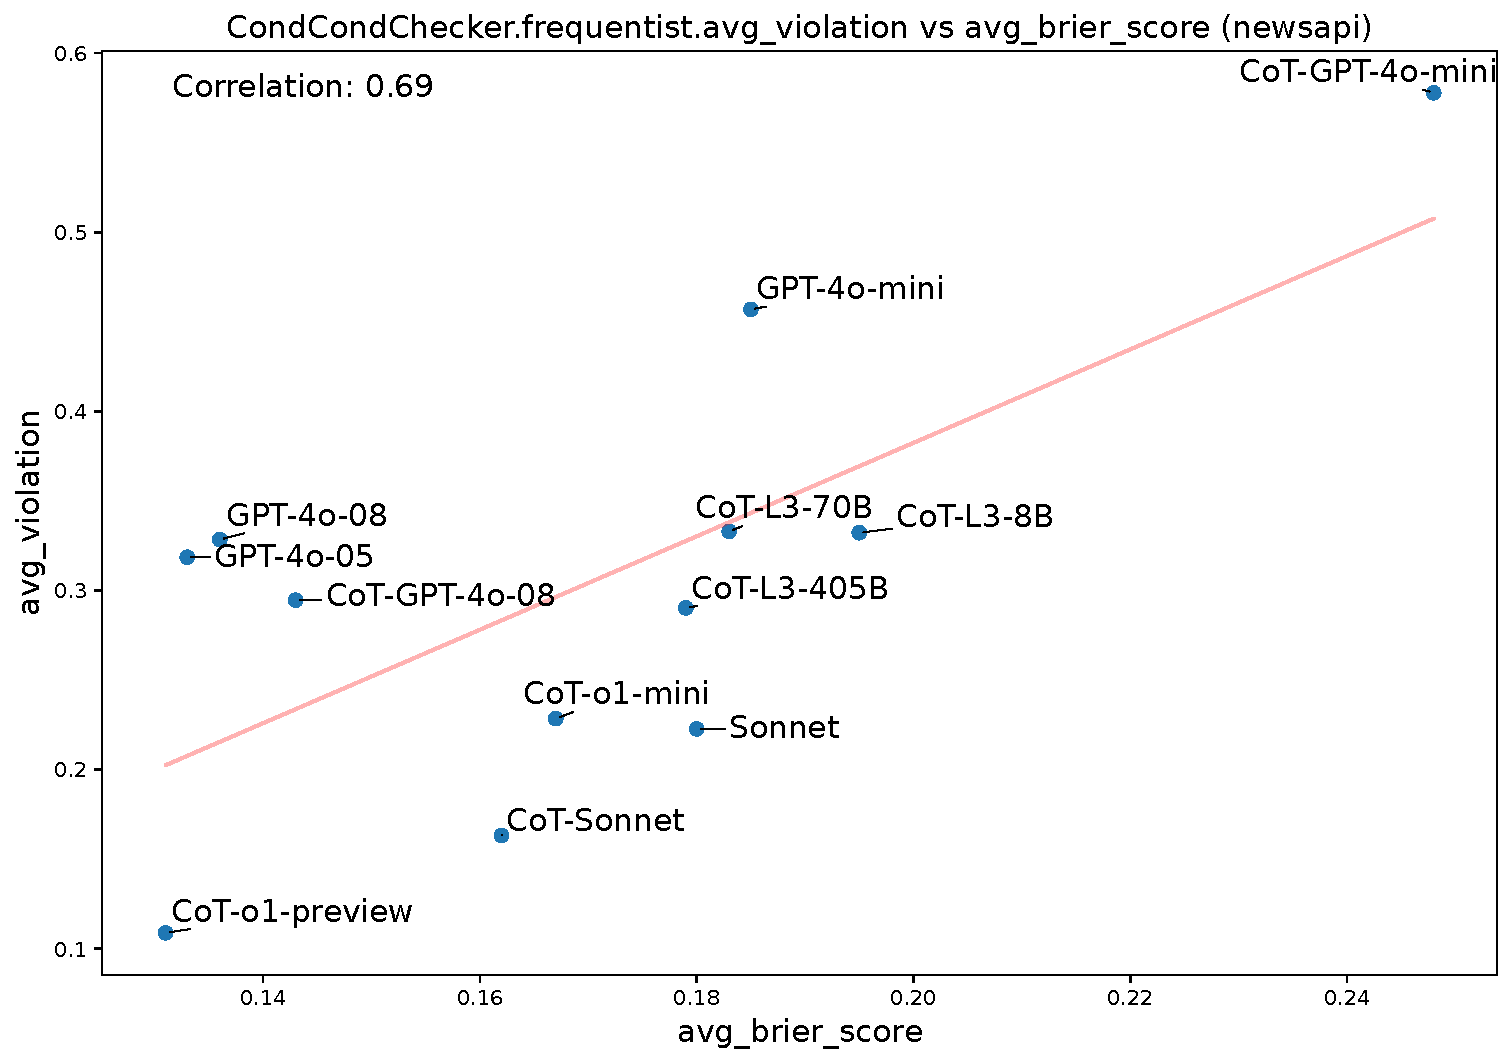
\includegraphics[width=\textwidth]{figures/consistency/CondCondChecker_vs_avg_brier_score_frequentist_avg_violation_newsapi.pdf}
        \caption{
        \CondCondChecker{} frequentist metric on the NewsAPI questions dataset.
        }
        \label{fig:condcondchecker_vs_brier_newsapi}
    \end{subfigure}
    \caption{
        Both \CondChecker{} and \CondCondChecker{} consistency metrics \rebuttal{see \Cref{tab:consistency_checks}} show a strong correlation with forecasting accuracy as measured by the Brier score.
    }
    \label{fig:consistency_vs_brier-condchecker}
\end{figure}


\textbf{Bayesian consistency checks are the best proxies for forecasting performance.}
Figure \ref{fig:condchecker_vs_brier_scraped} shows the strong correlation between certain consistency checks
\rebuttal{from \Cref{tab:consistency_checks}}
and average Brier scores across different forecasters.
This relationship suggests that \CondChecker{}, which tracks logical consistency in conditional probability estimates, serves as \rebuttal{a proxy} for overall forecasting accuracy, \emph{without knowing how the questions resolved}.


\textbf{Certain consistency metrics are not well correlated with forecasting performance.}
The measured correlations between the consistency checks and Brier scores are given in \Cref{tab:consistency-correlations}. We see that some checks yield higher signal on the ground truth performance than others.
Aggregating different consistency metrics seems to improve the correlation.

We note that the selection of forecasters we test is quite limited,
%(see \Cref{cfc/sec:cannot_evaluate_halawi})
so we cannot guarantee the trends here are representative of future LLM forecasters.
%trends here need to be taken with a grain of salt. \vin{refine - trends here should be taken as purely demonstrative.}
\rebuttal{Part of the correlation can be attributed to better models being both more consistent and better forecasters. For comparison, the correlations of the Brier score of our forecasters and the MMLU \cite{mmlu} (college split) error rate on the best approximation of the tested forecasters are 0.38 and 0.55 on the NewsAPI and scraped datasets, respectively.}

We include all data (questions, tuples, forecasts, and scores) in the supplementary material.

\begin{table*}[hbp]
    \centering
   \caption{Correlation of consistency metrics with Brier score, across both of our base question datasets and the derived consistency check tuples.}
   \label{tab:consistency-correlations}
   \small
   \begin{tabular}{lrrrr}
     \toprule
     & \multicolumn{2}{c}{Scraped} & \multicolumn{2}{c}{NewsAPI} \\
     \cmidrule(lr){2-3} \cmidrule(lr){4-5}
     & Arbitrage & Frequentist & Arbitrage & Frequentist \\
     \midrule
     \NegChecker{} & 0.60 & 0.67 & -0.36 & -0.13 \\
     \ParaphraseChecker{} & 0.57 & 0.61 & 0.13 & 0.24 \\
     \ConsequenceChecker{} & 0.51 & 0.52 & 0.21 & 0.30 \\
     \AndOrChecker{} & 0.20 & 0.25 & 0.02 & 0.06 \\
     \AndChecker{} & 0.68 & 0.72 & 0.54 & 0.71 \\
     \OrChecker{} & 0.14 & 0.24 & -0.24 & -0.31 \\
     \ButChecker{} & 0.20 & 0.67 & 0.63 & 0.77 \\
     \CondChecker{} & 0.92 & 0.87 & 0.71 & 0.69 \\
     \CondCondChecker{} & 0.78 & 0.71 & 0.75 & 0.69 \\
     \ExpectedEvidenceChecker{} & 0.20 & 0.77 & -0.11 & 0.06 \\
     Aggregated & 0.62 & 0.85 & 0.49 & 0.66 \\
     \bottomrule
   \end{tabular}
   \label{tab:consistency-correlations-2}
 \end{table*}


\textbf{Even good reasoning models are inconsistent.}
We give the full set of consistency metrics for OpenAI's \oonemini{} in \Cref{tab:o1-mini}.
The \texttt{Frac} column counts the fraction of tuples for which the violation exceeded a certain threshold; see the full exposition of what the thresholds mean in \Cref{cfc/app:arbitrage,cfc/app:frequentist-metric}.
The frequentist metric is not directly comparable to the arbitrage metric, but the respective violation counts (``Frac'' in the table) are.

%\adamunimp{these 2 paragraphs should be cut or moved.  Why are we explaining the cutoffs for the arbitrage metric and frequentist metric here?}For the arbitrage metric, this threshold is $10^{-2}$, corresponding to the arbitrage profit between two forecasts of $0.5$ and $0.6$ on \NegChecker{}.
%For the frequentist metric, this is determined by rejecting the null hypothesis of a Monte Carlo forecaster, at significance level $p<0.01$.
%The full exposition of the frequentist metric is in \Cref{cfc/app:frequentist-metric}.
%The violation threshold for the frequentist metric is chosen to be at the metric value of the $(0.5,0.6)$ pair for \NegChecker{}.


\begin{table*}[htbp]
\centering
  \caption{Consistency metrics for o1-mini.}
  \label{tab:o1-mini}
  \small
  \begin{tabular}{@{} lrrrrrrrr @{}}
    \toprule
    & \multicolumn{4}{c}{Scraped} & \multicolumn{4}{c}{NewsAPI} \\
    \cmidrule(lr){2-5} \cmidrule(lr){6-9}
    & \multicolumn{2}{c}{Arbitrage} & \multicolumn{2}{c}{Frequentist} & \multicolumn{2}{c}{Arbitrage} & \multicolumn{2}{c}{Frequentist} \\
    \cmidrule(lr){2-3} \cmidrule(lr){4-5} \cmidrule(lr){6-7} \cmidrule(lr){8-9}
    Check & Avg & Frac & Avg & Frac & Avg & Frac & Avg & Frac \\
    \midrule
    \NegChecker{} & $0.07$ & $58\%$ & $0.26$ & $61\%$ & $0.08$ & $52\%$ & $0.27$ & $56\%$ \\
    \ParaphraseChecker{} & $0.07$ & $56\%$ & $0.26$ & $61\%$ & $0.06$ & $53\%$ & $0.24$ & $56\%$ \\
    \ConsequenceChecker{} & $0.03$ & $27\%$ & $0.13$ & $29\%$ & $0.03$ & $18\%$ & $0.10$ & $19\%$ \\
    \AndOrChecker{} & $0.09$ & $65\%$ & $0.34$ & $71\%$ & $0.07$ & $57\%$ & $0.29$ & $67\%$ \\
    \AndChecker{} & $0.02$ & $24\%$ & $0.11$ & $27\%$ & $0.03$ & $23\%$ & $0.11$ & $24\%$ \\
    \OrChecker{} & $0.11$ & $48\%$ & $0.30$ & $50\%$ & $0.05$ & $48\%$ & $0.21$ & $50\%$ \\
    \ButChecker{} & $0.11$ & $60\%$ & $0.40$ & $79\%$ & $0.11$ & $63\%$ & $0.38$ & $80\%$ \\
    \CondChecker{} & $0.04$ & $41\%$ & $0.22$ & $52\%$ & $0.07$ & $66\%$ & $0.29$ & $70\%$ \\
    \CondCondChecker{} & $0.03$ & $30\%$ & $0.19$ & $45\%$ & $0.04$ & $54\%$ & $0.23$ & $71\%$ \\
    \ExpectedEvidenceChecker{} & $0.04$ & $47\%$ & $0.27$ & $69\%$ & $0.05$ & $45\%$ & $0.28$ & $63\%$ \\
    \midrule
    \textbf{Aggregated} & $0.06$ & $-$ & $0.25$ & $-$ & $0.06$ & $-$ & $0.24$ & $-$ \\
    \bottomrule
  \end{tabular}
\end{table*}
OpenAI's \oonemini{} forecaster, despite being one of the best reasoning models so far, violates consistency checks more than the $(0.5, 0.6)$ threshold from \Cref{cfc/sec:forecasting} very often.

% \textbf{Long-horizon consistency benchmark.}
% The results of the previous section indicate that, even on longer time horizons where it's not possible to have ground truth resolutions, we can still evaluate and compare different forecasters via consistency metrics.

% We create a dataset of 900 synthetic questions resolving in 2028 and create 3000 tuples in total from this dataset using the method described in \Cref{cfc/sec:instantiation}, to evaluate the consistency of the forecasters in questions with a longer horizon, where it's not
% possible to have the ground truth resolutions. Examples of questions and the results for \gptfouro{} are in \Cref{cfc/app:synthetic-questions-2028}.

% We intend this dataset as a working prototype for a continual long-term forecasting benchmark.
%\adamunimp{This section is kinda week.  Like who cares, you have a bunch of questions that willnot resolve in the near future.  If keep, at least mention how it can be useful as a continual benchmark for future studies}

\section{\CFCaster{}: Can we design a more consistent forecaster?}
\label{cfc/sec:cfcaster}

\rebuttal{Let $(x_1,\dots x_n)$ be a question tuple for some consistency check $\Relation$, e.g. $(P,\lnot P)$. Given forecasts $\Forecaster(x_1), ... \Forecaster(x_n)$, the arbitrage metric maximization problem in ~Equation ~\ref{eq:arbitrage__} computes the following (as the argmax and max of the arbitrage respectively):}

\begin{enumerate}
    \item Improved forecasts $\Forecaster'(x_1), ... \Forecaster'(x_n)$ which are consistent, i.e. satisfy $\CCheck$; and
    \item The profit earned by an arbitrageur who bets these improved forecasts against the original ones -- this is the actual metric.
\end{enumerate}

This leads us to wonder: \emph{can we use these ``improved consistent forecasts'' to build a new forecaster which builds on the base forecaster $\Forecaster$, but is more consistent on $\Relation$}?

We introduce: the \CFCaster{} with base $\Forecaster$ arbitraged on consistency check $\Relation$, denoted by $\CFC[\Relation]{\Forecaster}$, which computes its forecast on a question $x$ as follows:
\begin{enumerate}
    \item Instantiates a tuple $(x_1,\dots x_n)$ satisfying $\Relation$;
    \item Queries $\Forecaster$ to obtain $\Forecaster(x_1),\dots\Forecaster(x_n)$;
    \item Arbitrages these base forecasts per Eq~\ref{eq:arbitrage__} and returns the arbitraged forecast for $x_1$.
\end{enumerate}

\rebuttal{Despite what one might assume, however, an \CFCaster{} is \emph{not} ``definitionally'' consistent on the check it is arbitraged on, but rather its consistency must be investigated empirically. Suppose, for example, that a forecaster produces forecasts $\Forecaster(P)=0.5$, $\Forecaster(\operatorname{para}(P))=0.6$, $\Forecaster(\operatorname{para}(\operatorname{para}(P)))=0.7$. Then $\Forecaster':=\CFC[\ParaphraseChecker{}]{\Forecaster}$ would produce forecasts $\Forecaster'(P)\approx0.55$, $\Forecaster'(\operatorname{para}(P))\approx0.65$, which are not consistent.}

Appendix~\ref{cfc/app:cfcaster} contains a precise definition of \CFCaster{}, including the case of sequentially arbitraging on multiple checks $\CFC[[\Relation_1,\dots\Relation_s]]{\Forecaster}$, and a theoretical discussion of its consistency properties. In particular, we list strong theoretical reasons to expect consistency gains from \emph{recursive} \CFCaster{} setups, i.e. $\CFC[\Relation]{\Forecaster}^r:=\CFC[\Relation]{\CFC[\Relation]{\Forecaster}^{r-1}}$, in particular with \NegChecker{}, as well as in a non-recursive \CFCaster{} with \ExpectedEvidenceChecker{}.

Due to these priorities and the high costs of running recursive \CFCaster{}s (see Appendix~\ref{cfc/app:cfcaster-cost}), we limited ourselves to studying only a small number of \CFCaster{} setups, with a limited number of checks rather than the whole list; specifically: $\CFC[N]{g}^r$, $\CFC[P]{g}^r$, $\CFC[[N,P]]{g}^r$, $\CFC[[E]*s]{g}$ where $g:=$\gptfouromini{}, $N,P,E$ are \NegChecker{}, \ParaphraseChecker{}, \ExpectedEvidenceChecker{} respectively, and $r$ and $s$ vary from 0 to 4.

% A single call to $\CFC[\vec{C}]{\Forecaster}$ involves $1+\sum_i (n_{\Relation_i}-1)$ calls to $\Forecaster$, plus several LLM calls for each $\FullInstantiator_i$ depending on the exact instantiation process (see Appendix~\ref{cfc/app:cfcaster-cost} for details) -- running this for all checks in Table~\ref{tab:consistency_checks} can get quite expensive, especially for the recursive \CFCaster{}s we are interested in. Thus in our experiments we limited ourselves to studying only a small number of \CFCaster{} setups, with a limited number of checks, specifically we experimented with: $\CFC[N]{g}^r$, $\CFC[P]{g}^r$, $\CFC[[N,P]]{g}^r$, $\CFC[[E]*r]{g}$ where $g:=$\gptfouromini{}, $N,P,E$ are \NegChecker{}, \ParaphraseChecker{}, \ExpectedEvidenceChecker{} respectively, and $r$ varies from 0 to 4.
% \begin{itemize}
%     \item $\CFC[\NegChecker{}]{\gptfouromini{}}^r$ (denoted in tables and plots as CF-Nr)
%     \item $\CFC[\ParaphraseChecker{}]{\gptfouromini{}}^r$ (denoted in tables and plots as CF-Pr)
%     \item $\CFC[[\NegChecker{},\ParaphraseChecker{}]]{\gptfouromini{}}^r$ (denoted in tables and plots as CF-NPr)
%     \item $\CFC[[\ExpectedEvidenceChecker{}]*r]{\gptfouromini{}}$ (denoted in tables and plots as CF-rxEE1)
% \end{itemize}

The full results of our experiments with these forecasters are reported in Appendix~\ref{cfc/app:cf-results}; our key takeaways from these preliminary runs look hopeful:

\begin{itemize}
    \item In the case of the checks we tested, \textbf{arbitraging on a check indeed makes a forecaster more consistent on that check}\vin{change to emph rather than textbf}, with increasing consistency gains with recursive depth, as shown in Fig~\ref{fig:cf-4}. Crucially, this also applied when the arbitraging was on more than a single check: $\CFC[[N,P]]{g}^r$ did well on \emph{both} \NegChecker{} and \ParaphraseChecker{}; arbitraging on the next check did not increase inconsistency on the first. We are cautiously optimistic that this may extend to the full list of checks in Table~\ref{tab:consistency_checks}.
   % once cost does not deter from testing it.
    %\manyu{not sure if this list sounds like too much inference based on too little}
    %\adamunimp{But it also made all of the other ones worse. should that be mentioned?}
    %\dpaleka{It made some of the other ones better and some worse}
    \item \textbf{This consistency gain was greatest with \NegChecker{}, followed by \ParaphraseChecker{}, and lowest with \ExpectedEvidenceChecker{}.} This finding is in line with our hypothesis in Appendix~\ref{cfc/app:cfcaster} that \CFCaster{} would be particularly effective on consistency checks which are \emph{symmetric}. and instantiate \emph{deterministically}.
    %\adamunimp{not sure how much this line adds}
    \item \textbf{We do not observe reliable improvements on ground truth forecasting performance, or on consistency checks other than the ones we arbitrage on.}
%    \adamunimp{again it actually does worse...My guess is that in trying to fix one parameter, it ignores the constraints of the others}
%    \dpaleka{it's not always worse, e.g. for \CondChecker{} it increases twice and decreases twice}
    I.e. $\CFC[\Relation_1]{\Forecaster}$ does not reliably do better on $\Relation_2$.
\end{itemize}

\begin{figure}[h]
    \centering
    \begin{subfigure}[b]{0.46\textwidth}
        \centering
        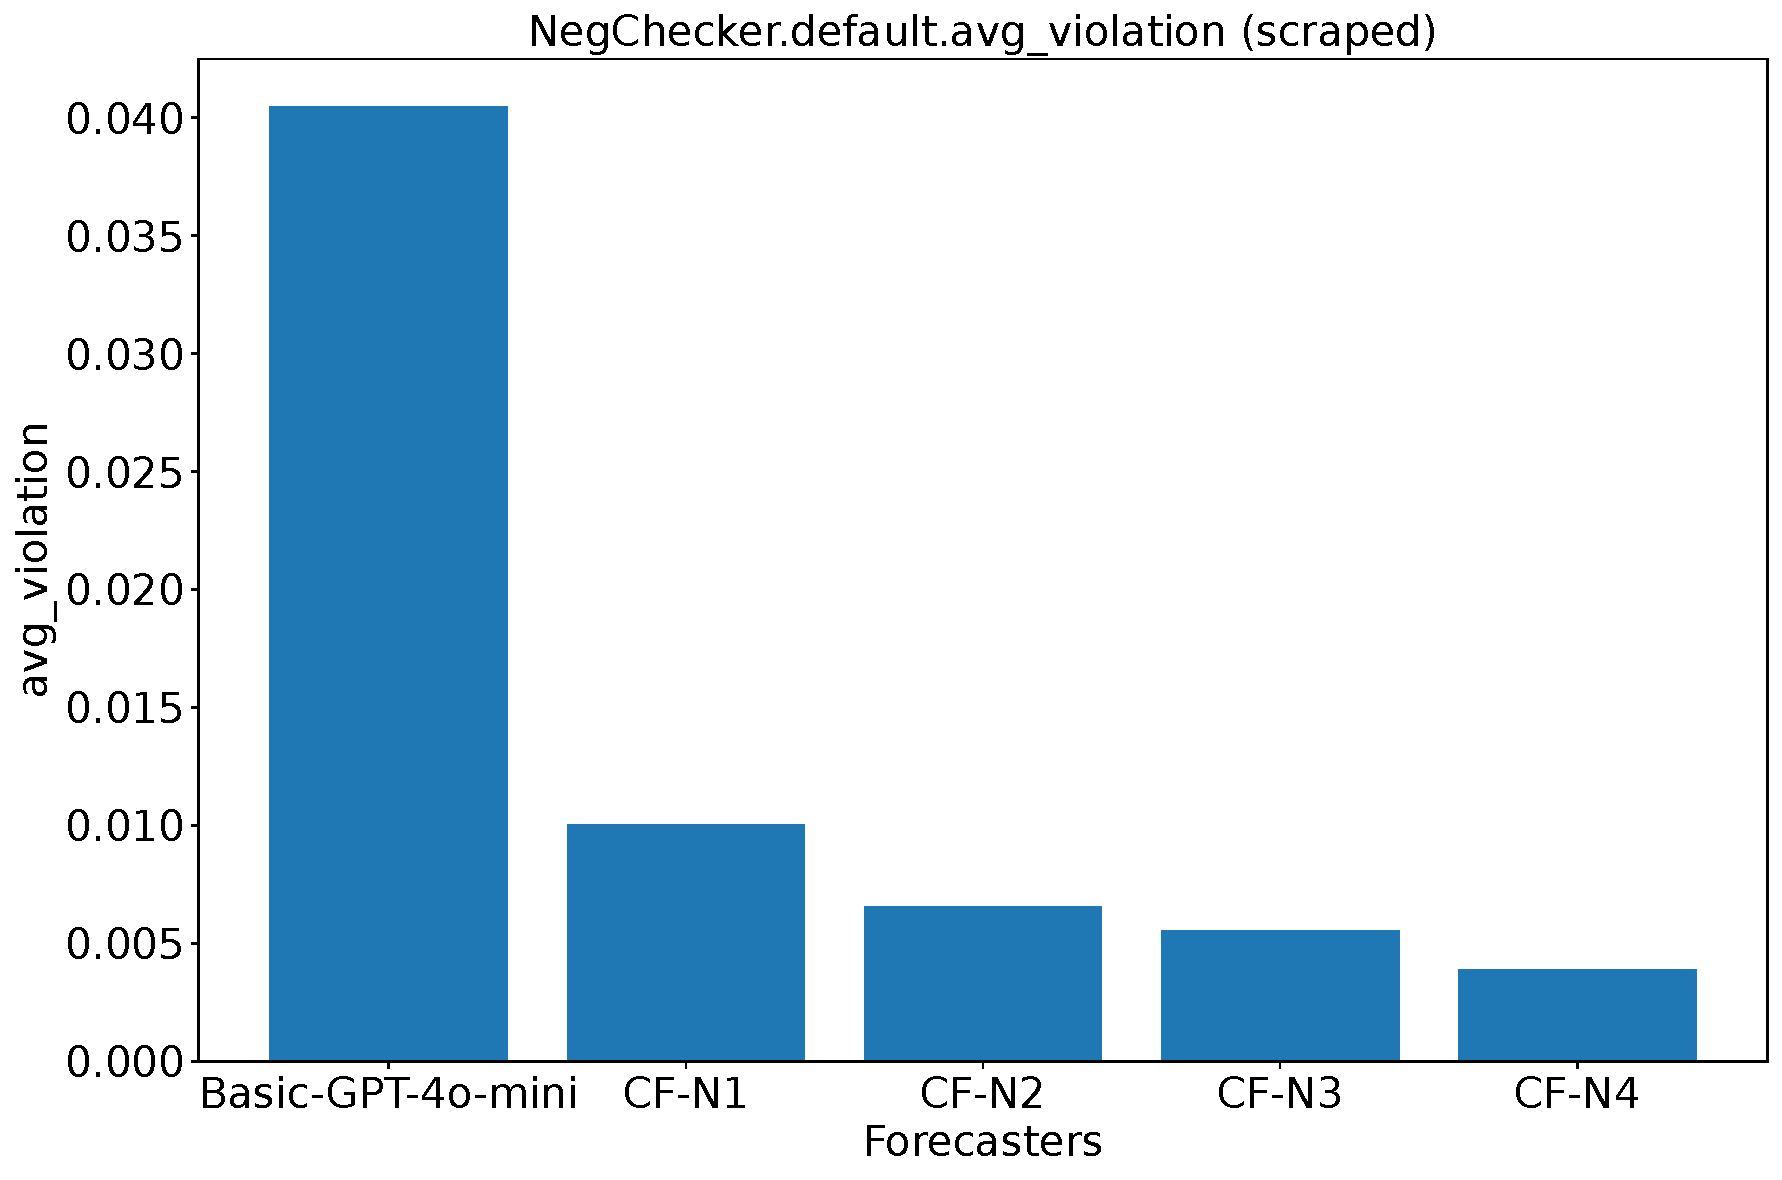
\includegraphics[width=\textwidth]{figures/consistency/cfcaster_scraped/N-N.pdf}
        \caption{Average violation of $\CFC[N]{g}^r$ (denoted CF-Nr) on \NegChecker{} for $r$ from 0 to 4.
        }
        \label{fig:N-N}
    \end{subfigure}
    \hfill
    \begin{subfigure}[b]{0.48\textwidth}
        \centering
        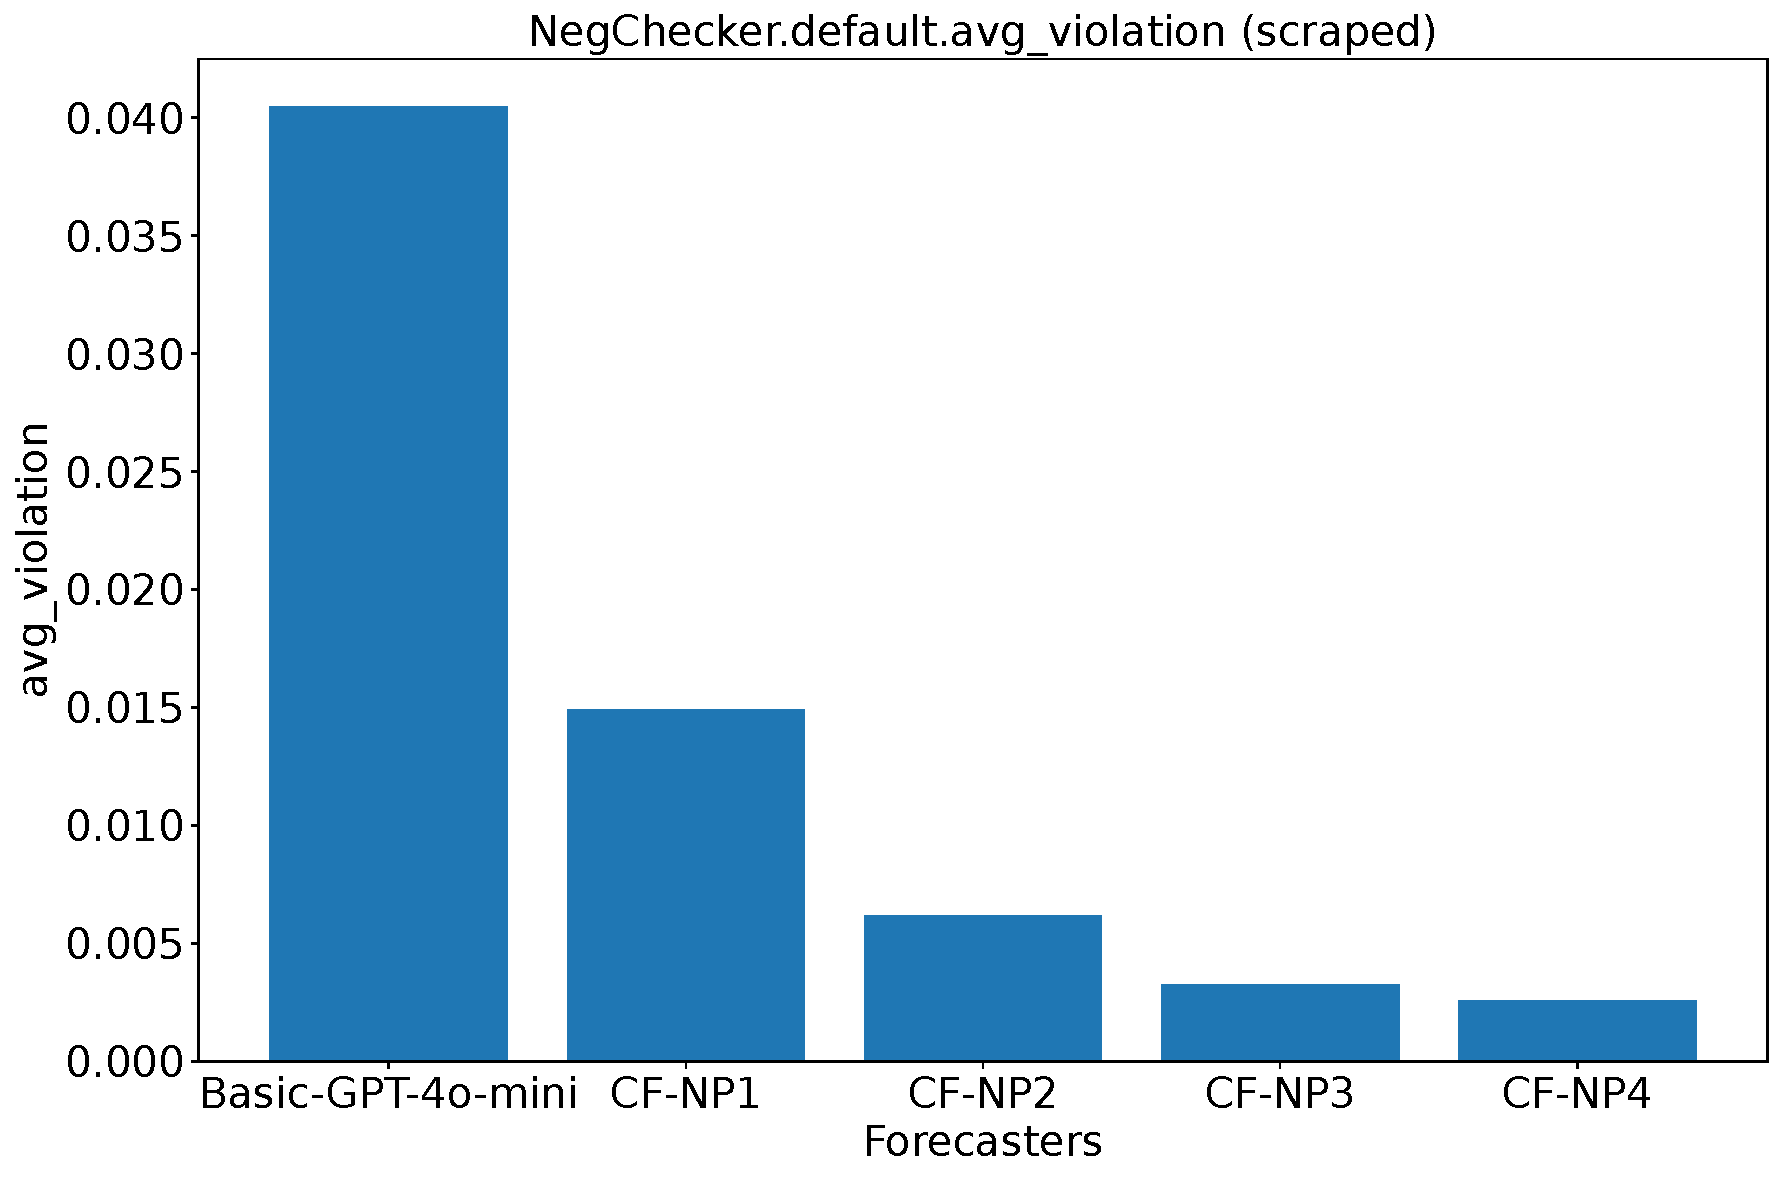
\includegraphics[width=\textwidth]{figures/consistency/cfcaster_scraped/NP-N.pdf}
        \caption{Average violation of $\CFC[NP]{g}^r$ (denoted CF-NPr) on \NegChecker{} for $r$ from 0 to 4.
        }
        \label{fig:NP-N}
    \end{subfigure}
    \begin{subfigure}[b]{0.48\textwidth}
        \centering
        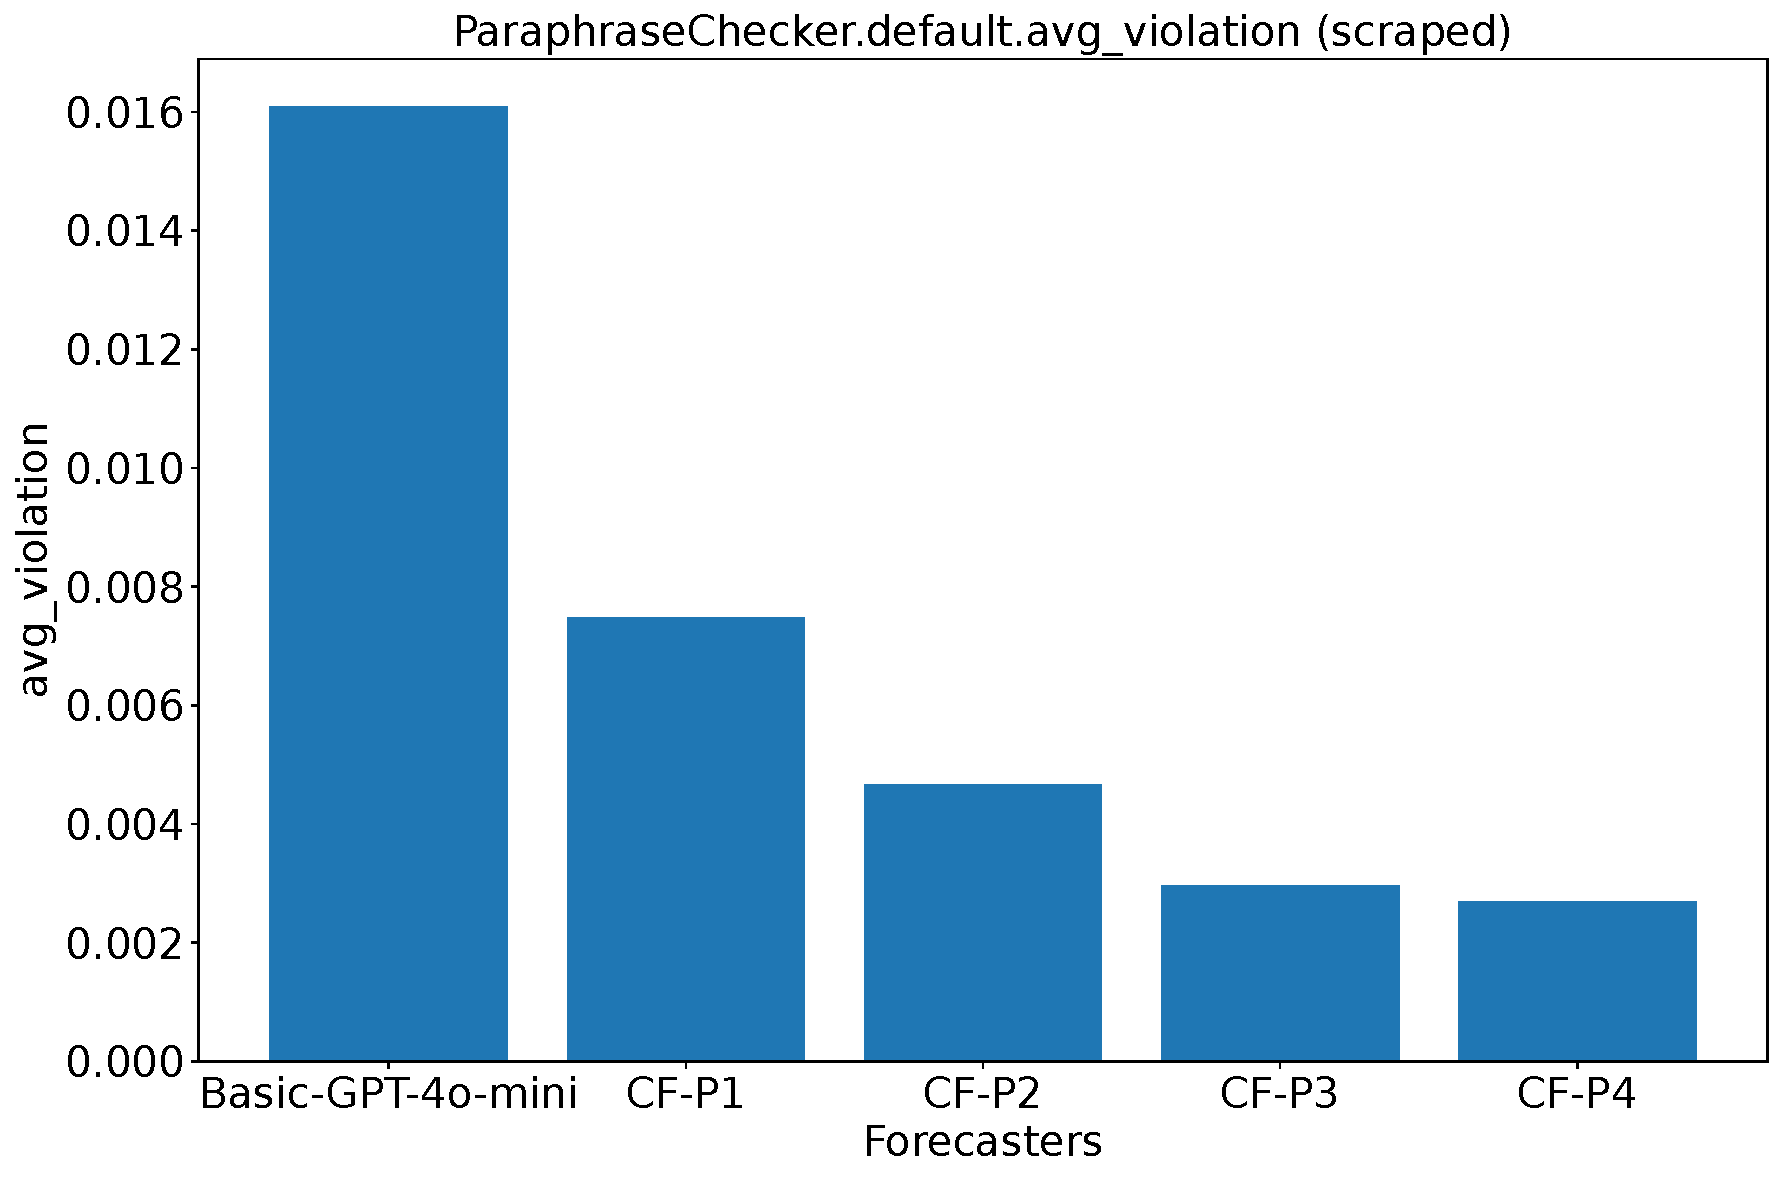
\includegraphics[width=\textwidth]{figures/consistency/cfcaster_scraped/P-P.pdf}
        \caption{
         Average violation of $\CFC[P]{g}^r$ (denoted CF-Pr) on \ParaphraseChecker{} for $r$ from 0 to 4.}
        \label{fig:P-P}
    \end{subfigure}
    \hfill
    \begin{subfigure}[b]{0.48\textwidth}
        \centering
        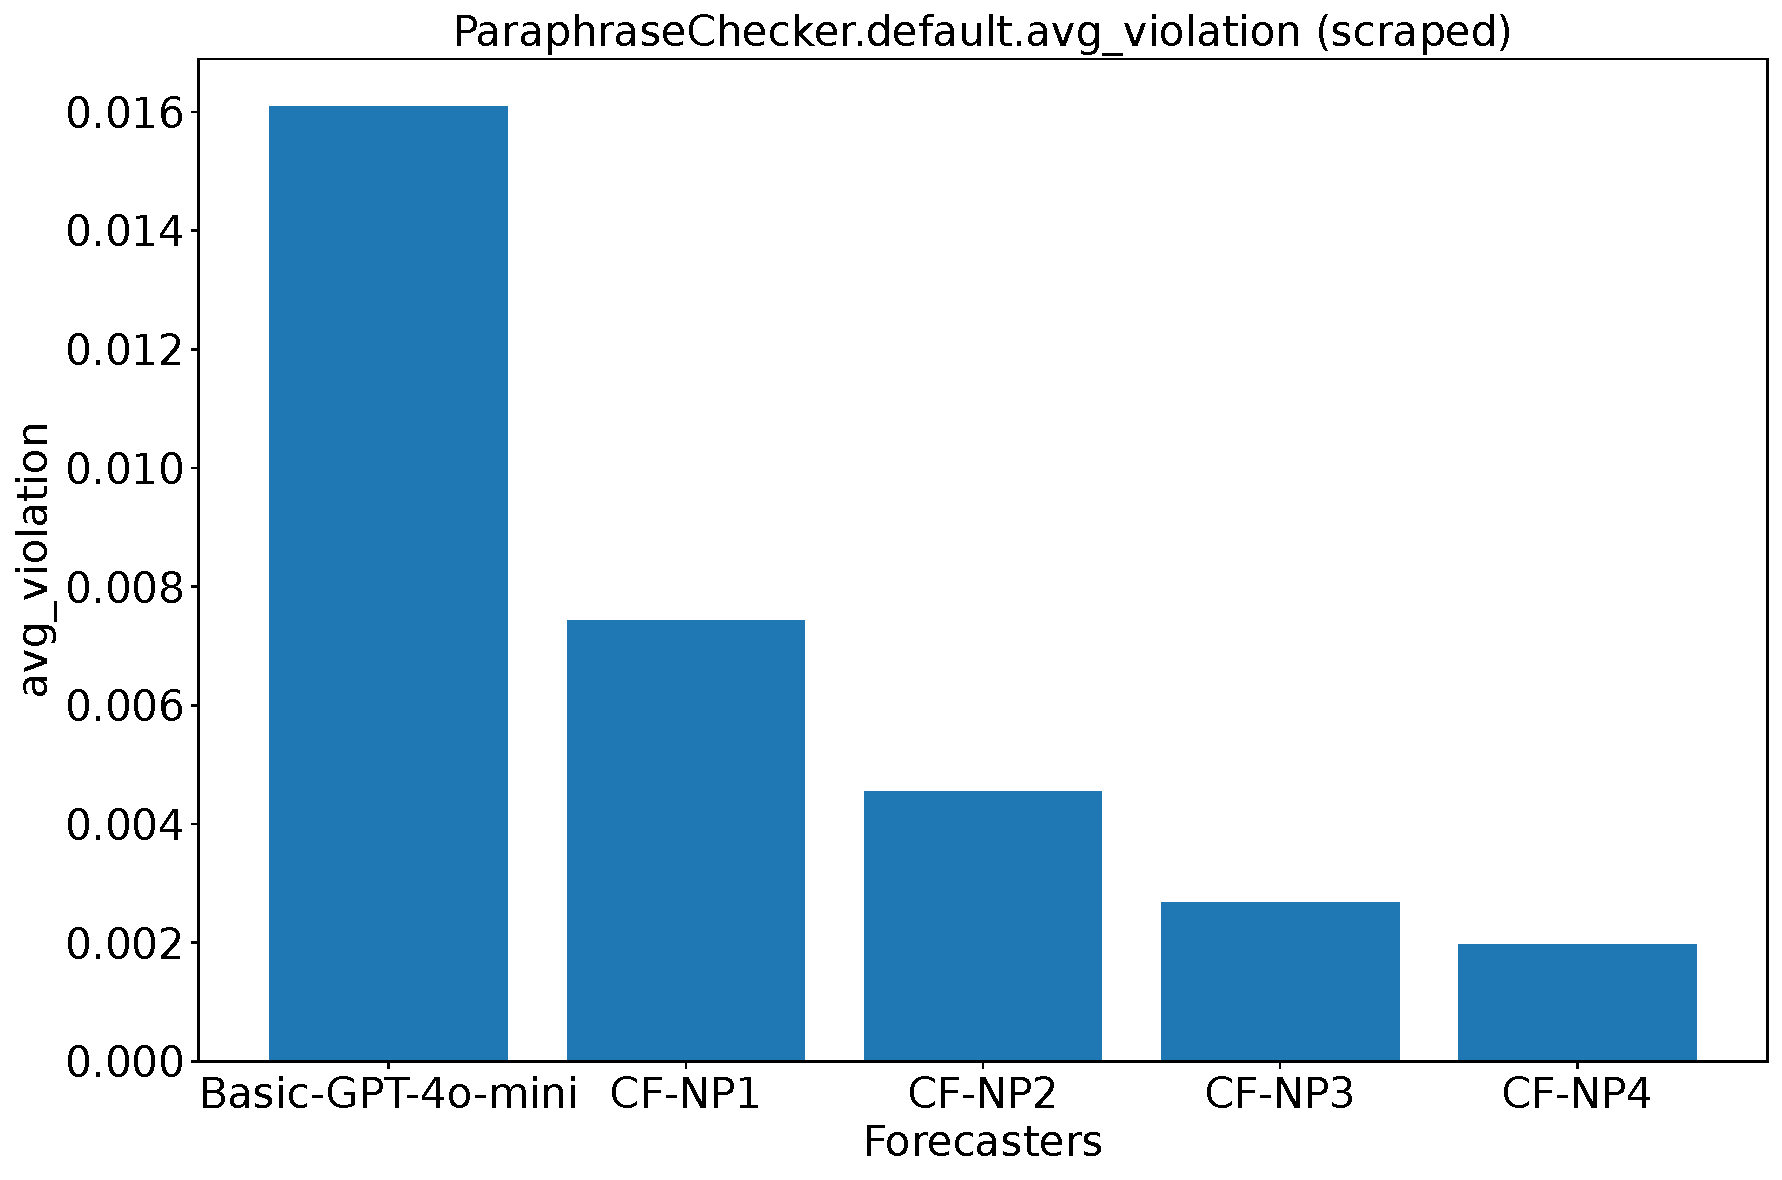
\includegraphics[width=\textwidth]{figures/consistency/cfcaster_scraped/NP-P.pdf}
        \caption{
         Average violation of $\CFC[NP]{g}^r$ (denoted CF-NPr) on \ParaphraseChecker{} for $r$ from 0 to 4.}
        \label{fig:NP-P}
    \end{subfigure}
    \caption{\NegChecker{} and \ParaphraseChecker{} violations for various \CFCaster{} setups. In all captions, $g$ denotes \gptfouromini{}, $N,P$ denote \NegChecker{} and \ParaphraseChecker{} respectively, and the definition of the \CFCaster{} setup is as in Def~\ref{def:cf}.}
    \label{fig:cf-4}
\end{figure}


\section{Related work}
\textbf{Metamorphic and consistency checks.}
Checking logical properties of outputs of programs under semantic-preserving transforms has a long history \citep{chen1998metamorphic}. Before \citet{esmwcc}, variants of the consistency check framework were used for simple ML models \citep{christakis2022specifying, sharma2020monotonicity}, vision \citep{hendrycks2019benchmarking}, and chat LLMs \citep{jang2023consistency}, among other areas.
\rebuttal{
\citet{li2019logic} consider logical consistency checks beyond paraphrasing and negation for simple ML models.
}
%Evaluating without ground truth in a fashion similar to this a long history as \emph{metamorphic testing} ...
%\todo{@dpaleka finish}

\textbf{Forecasting and large language models.}
LLMs and forecasting date back to \citet{zou2022forecasting} and \citet{yan2023autocast++}. Recently, strong performance of LLM forecasters on prediction market datasets has been claimed in \rebuttal{\citep{halawiApproachingHumanLevelForecasting2024, tetlock2024longrange, hsieh2024reasoning, safeai2024forecasters}}.
\rebuttal{
Concurrent with our work, \citet{karger2024forecastbench} have introduced an automatically updating benchmark for forecasting.
}

\textbf{Scalable oversight and failures of superhuman AI.}
The difficulty of evaluating models with superhuman performance in domains without a source of ground truth has long been acknowledged, and falls under the umbrella of \emph{scalable oversight}  \citep{amodei2016concrete}.
Forecasting using AI oracles is one such domain.  The use of consistency checks for scalable oversight has been studied in the simpler context of superhuman game AIs \citep{alphazero_not_robust, esmwcc},
and in general question-answering tasks via debate \citep{irving2018debate}.

\textbf{Consistency evaluations for LLMs.}
Even on tasks where the ground truth is in principle knowable,
consistency evaluations have long helped in cases where checking consistency is easier than getting the ground truth labels \citep{elazarPararel2021, liGeneratorValidatorConsistency2023}.
\rebuttal{
\citet{raj2023semantic} measure paraphrasing consistency and ground truth accuracy on TruthfulQA \citep{lin2021truthfulqa} and find little to no  correlation.
}
Some forms of consistency checks have been applied on model internals to discover features related to LLM truthfulness and reliability \citep{burnsDiscoveringLatentKnowledge2022, kaarelSearchingModelsConcepts2023}.


%{Failure modes in superhuman models.}
%ML models achieve undisputed superhuman performance for various games, e.g., chess~\cite{campbell2002deep, alphazero} or Go~\cite{alphago}.
%%\footnote{ML models also surpass human baselines on some benchmarks for vision, speech or natural language processing, but we do not consider these models as superhuman here, as the ground truth for these tasks is still defined from human knowledge.}
%Yet, game-playing agents for Go can be defeated by simple adversarial strategies designed against them~\cite{alphazero_not_robust, go_adversarial, go_adversarial2}.
%These strategies are either found ``end-to-end'' (via self-play against the victim)~\cite{go_adversarial, go_adversarial2},
%or by checking consistency over boards that appear semantically equivalent to an examiner (either a human observer or a stronger model)~\cite{alphazero_not_robust}.
%In contrast, we consider the problem of eliciting bugs in model decisions when a proxy for ground truth (better than the model being evaluated) is not available.
%{Scalable oversight.} Our work relates to the problem of \emph{scalable oversight}~\cite{amodei2016concrete},
%the ability to supervise models when  ground truth is hard or impossible to obtain (e.g., because model abilities match or exceed humans).
%Our work is complementary to prior methods, which make capable models and humans interact to extract confidently correct answers~\cite{bowman2022measuring, irving2018debate};
%we instead study how humans could probe such models for confidently \emph{incorrect} answers, i.e., human-verifiable bugs.
%
%{Model truthfulness.}
%There are many attempts at evaluating the truthfulness of language model outputs~\cite{evans2021truthful, lin2021truthfulqa}.
%%Our consistency checks can be viewed as a way of demonstrating model falsehoods in the absence of known ground truth.
%We envision that consistency tests could serve as a method for detecting when models provide dishonest answers or lies~
%\cite{burtell2023artificial, cicero-diplomacy, pan2023rewards, burns2022discovering, christiano2022elk},
%under the assumption that it is easier to provide consistent answers when telling the truth~\cite{irving2018debate}.

%\citet{liGeneratorValidatorConsistency2023} check consistency of LLMs are  \emph{generators} (``Write a sentence funnier than sentence X'') and \emph{validators} (``Is sentence X or Y funnier?'').
%This paradigm is applicable for a general AI system forecasting: we can use ``Give me an event which is more likely to happen than event X'' as a generator, and check the probabilities afterward.


\section{Future work}
\label{cfc/sec:future-work}
%\dpaleka{This section can be very short if needed}

We have developed a comprehensive benchmark of \emph{static consistency checks} for LLM forecasters, and demonstrated its correlation with ground truth accuracy, suggesting that our consistency metrics could serve as a proxy for accuracy when we do not have access to ground truth. We envision several directions in which our framework could be extended:

% summary

%\todo{rephrase probably, and maybe add some speculative idea that uses CCS}
%We foresee several promising directions:

\textbf{Consistency in decision-making.} AI systems may be used not only to make forecasts that inform decisions, but also to take decisions directly. Here too, we can have a notion of inconsistency: for example, \emph{intransitive preferences}
\footnote{See e.g. \cite{fishburnUtilityTheoryDecision1970} and the Von Neumann–Morgenstern utility theorem for an introduction to decision rationality.} -- and analogously, an inconsistent decision-maker may be exploited by an arbitrageur.

%We can think of an AI decision-maker as giving utility estimates to different options (and choosing the highest one), much like an AI forecaster gives probability estimates to different outcomes. However, the analogy is not completely straightforward, as AI decision makers may also differ on which options they list in their analysis. %A similarly thorough benchmark for decisional consistency will require some nontrivial insights on such considerations.

\textbf{Training for consistency.~}
Modulo consideration of the cost-benefit to safety,
our methods could be used train LLMs for consistency,
minimizing our violation metrics.
This may or may not impact overall forecasting performance and other AI capabilities.
%as well as measure if this improves truthfulness overall, e.g. by comparing answers to the model's internal beliefs.
One may also imagine an AlphaZero-style set-up, where an LLM $\Forecaster$ is trained on the outputs of $\CFC{\Forecaster}^r$, i.e. a recursive \CFCaster{} wrapped around it.

\rebuttal{\textbf{Further experiments with \CFCaster{}.} Most of our experiments with \CFCaster{} involved arbitraging on only a \emph{single} check (apart from one experiment with both \NegChecker{} and \ParaphraseChecker{}), due to the cost limitations described in \ref{cfc/app:cfcaster-cost}. It is easy to imagine how a bad forecaster could still overfit a single check: simply forecasting $50\%$ probability for all questions will pass \ParaphraseChecker{}, \ExpectedEvidenceChecker{} and  \NegChecker{} -- but we expect that being consistent under a variety of checks is difficult without a consistent world model. One approach to using more checks cheaply, particularly in training, may be to \emph{randomly sample} a number of consistency checks for each question.}

\textbf{Dynamic generation of consistency checks.~}
Although we found strong correlations between ground truth accuracy and consistency among existing LLM forecasters, our results with \CFCaster{} demonstrate that this isn't necessarily the case: it is possible to do well on consistency without improving ground truth. In particular, this means that consistency as a training metric could be ``Goodharted'' by a learning AI model \citep{karwowskiGoodhartsLawReinforcement2023}. One way to prevent this may be via adversarial training: i.e. have an adversarial agent instantiate consistency checks that it believes the agent will perform poorly on.

%via Contrast-Consistent Search \cite{burnsDiscoveringLatentKnowledge2022a}.
%\todo{does this make sense? @dpaleka}

%\textbf{Performative prediction.} what if the world model is nontrivially influenced by the forecaster's answer \todo{dpaleka this was your idea; you should explain it}
%

\textbf{Evaluating RAG-augmented forecasters.~}
\label{cfc/sec:cannot_evaluate_halawi}
We have conducted some preliminary experiments evaluating state-of-the-art forecasters such as \cite{halawiApproachingHumanLevelForecasting2024}.
% [we acknowledge the help of Danny Halawi in adapting this]
Unfortunately, we could not reproduce the system from \cite{halawiApproachingHumanLevelForecasting2024} at the time of writing, due to deprecations in the Google News API (we could not obtain access to the alternative Newscatcher API).
At the time of writing, we are not aware of other publicly-available LLM forecasting systems that are competitive with the results of \cite{halawiApproachingHumanLevelForecasting2024}
(there exist proprietary systems that may be competitive, such as \cite{futuresearch2024}).
We thus leave the evaluation of better forecasters like \cite{halawiApproachingHumanLevelForecasting2024} and \cite{safeai2024forecasters} to future work, once such forecasters are more widely available.
%The main contribution of this work is a benchmark, not developing a new forecasting system.



%\begin{enumerate}
%    \item Ground truth forecasting results:
%    \begin{itemize}
%        \item Contains a JSONL file where each entry specifies:
%        \begin{itemize}
%            \item The question with a boolean \texttt{resolution} field
%            \item The forecasted probability and forecast metadata like chain of though traces
%            \item The obtained Brier score and other metrics
%        \end{itemize}
%        \item The total Brier score can be obtained by averaging individual scores.
%    \end{itemize}
%
%    \item Consistency checks results:
%    \begin{itemize}
%        \item Contains a JSONL and a JSON file for each consistency check:
%        \begin{enumerate}
%            \item Raw results file, where each entry is a tuple of questions with the forecast for each question, along with forecast metadata like chain of thought traces;
%            \item Summary statistics file, which statistics like average violation.
%        \end{enumerate}
%    \end{itemize}
%\end{enumerate}


\section*{Contributions}
\label{cfc/app:contributions}

DP and APS developed consistency checks and the arbitrage and frequentist metrics.
DP, AA, APS, and EW worked on the LLM question to evaluation pipeline.
APS thought of and implemented \CFCaster{}.
VB created the news-derived question dataset.
AS and DP created the scraped question dataset.
AA and DP created the 2028 synthetic question dataset.
DP started and led the project.
FT proposed correlating consistency with forecasting accuracy and advised the project.
All authors helped with the writing.
DP and APS wrote the first draft of the paper.

\section*{Acknowledgements}
We thank Danny Halawi for extensive discussions and help with our setup. We thank Brendan Murphy, Ezra Karger, Fred Zhang, and Tatsunori Hashimoto for helpful discussions and feedback on the paper and forecasting in general.
We thank Berkeley SPAR for connecting collaborators, and BERI for partially funding the project.

% \appendix

% \begin{appendix}
\section{Appendix}
\subsubsection{Table of consistency checks}
\label{cfc/app:checks}

Table~\ref{tab:full-consistency_checks} (extended version of Table~\ref{tab:consistency_checks}) includes all the consistency checks tested for in our benchmark. In most of them, we leave the logical relations between forecasting questions $\Relation$ implicit by constructing the sentences directly. For instance, $\Relation(x_1,x_2):=x_1=\lnot x_2$ is implied by simply writing $x_1, x_2$ as $P, \lnot P$. In the rest of the appendix, we use the sentence-based ($P, Q$ instead of $x_1, x_2$) notation. %\todo{is this extending beyond the margins?}

\begin{table*}[hbtp]
    \centering
    \caption{Consistency checks and the logical consistency conditions.}
    \vspace{5pt}
    \label{tab:full-consistency_checks}
    % \begin{tabular}{l p{3.7cm} p{7cm}}%{|l|p{6cm}|p{6cm}|}
    \begin{tabular}{l p{0.25\linewidth} p{0.4\linewidth}}
    \toprule
    \textbf{Name} &
    \textbf{Tuple} &
    \textbf{Condition ($\CCheck$)}
    %& \textbf{Violation Metric ($\Violation$)}
    \\ \midrule
    %\\ \hline
    \NegChecker &
    $(P,\lnot P)$ &
    $\Forecaster(P)+\Forecaster(\lnot P)=1$
    \\ \midrule
    \begin{tabular}{@{}l@{}} \ParaphraseChecker\\ $\Relation(P,Q):=P\iff Q$\end{tabular} &
    $(P,Q)$&
    $\Forecaster(P)=\Forecaster(Q)$
    \\ \midrule
    \begin{tabular}{@{}l@{}} \ConsequenceChecker\\ $\Relation(P,Q):=P\implies Q$\end{tabular} &
    $(P,Q)$&
    $\Forecaster(P)\le\Forecaster(Q)$
    \\ \midrule
    \AndOrChecker &
    $(P,Q,P\land Q,P\lor Q)$ &
    $\Forecaster(P)+\Forecaster(Q)=\Forecaster(P\lor Q)+\Forecaster(P\land Q)$
    \\ \midrule
    \AndChecker &
    $(P,Q,P\land Q)$ &
    $\max(\Forecaster(P)+\Forecaster(Q)-1, 0) \le \Forecaster(P\land Q) \le \min(\Forecaster(P),\Forecaster(Q))$
    \\ \midrule
    \OrChecker &
    $(P,Q,P\lor Q)$ &
    $\max(\Forecaster(P),\Forecaster(Q))\le\Forecaster(P\lor Q)\le\min(1,\Forecaster(P)+\Forecaster(Q))$
    \\ \midrule
    \ButChecker &
    $(P,\lnot P\land Q, P\lor Q)$ &
    $\Forecaster(P\lor Q)=\Forecaster(P)+\Forecaster(\lnot P\land Q)$ %
    \\ \midrule
    % \SymmetryAndChecker & $\Forecaster(P\land Q)=\Forecaster(Q\land P)$
    % \\ \midrule
    % \SymmetryOrChecker & $\Forecaster(P\lor Q)=\Forecaster(Q\lor P)$
    % \\ \midrule
    \CondChecker &
    $(P,Q|P,P\land Q)$ &
    $\Forecaster(P)\Forecaster(Q|P)=\Forecaster(P\land Q)$
    \\ \midrule
    %\CondCondChecker &
    %$(P,Q|P,R|(P\land Q),P\land Q\land R)$ &
    %$\Forecaster(P)\Forecaster(Q|P)\Forecaster(R|P\land Q) =\Forecaster(P\land Q\land R)$
    \CondCondChecker &
    \begin{tabular}[t]{@{}p{3.7cm}@{}}
    $(P,Q|P,R|(P\land Q),$\\
    $P\land Q\land R)$
    \end{tabular} &
    $\Forecaster(P)\Forecaster(Q|P)\Forecaster(R|P\land Q) =\Forecaster(P\land Q\land R)$
    \\ \midrule
    \ExpectedEvidenceChecker &
    $(P,Q,P|Q,P|\lnot Q)$&
    $\Forecaster(P)=\Forecaster(P|Q)\Forecaster(Q)+\Forecaster(P|\lnot Q)(1-\Forecaster(Q))$
    \\ \bottomrule
    \end{tabular}
\end{table*}

The consistency checks in Table~\ref{tab:full-consistency_checks} represent core logical relationships between probabilities, but many other forms of consistency checks are possible. Here are two examples that could extend our framework:

\begin{itemize}
    \item \textbf{Comparative checks:} Building on generator-validator checks from \citet{liGeneratorValidatorConsistency2023}, we could ask a forecaster to predict both $\Forecaster(P)$, $\Forecaster(Q)$, and separately whether $P$ or $Q$ is more likely. The forecaster's probability estimates should match their comparative judgment.

    \item \textbf{Monotonicity checks:} \citet{esmwcc} propose a variant of \ConsequenceChecker{} for real-valued quantities, where predictions must respect the monotonic ordering of a sequence of future values. \rebuttal{This connects to \emph{scope insensitivity} \citep{kahneman2000economic}, a cognitive bias where humans fail to scale probability estimates appropriately with the magnitude of outcomes.}
\end{itemize}

We do not include a specific consistency check for Bayesian updates, as conditional probabilities are already covered by \CondChecker{}, \CondCondChecker{}, and \ExpectedEvidenceChecker{}.

\subsubsection{Arbitrage as a violation metric}
\label{cfc/app:arbitrage}

\rebuttal{For the following definition we use a slightly more general notation than in the main body, to convey that our methods could be generalized beyond binary forecasting questions. }

\begin{notation*}

    \rebuttal{Let $\ForecastingQuestions$ denote the set of forecasting questions we are interested in, $\Resolutions$ denote the set of possible outcomes/resolutions for an individual question, and $\Forecasts$ denote the set of probability distributions on $\Resolutions$. A \emph{Forecaster} is a map $\Forecaster:\ForecastingQuestions\to\Forecasts$. For conditional questions that can resolve to $\none$, we also have optional resolutions $\ResolutionsOpt:=\Resolutions\cup\{\none\}=\boolsopt$.}
\end{notation*}


The arbitrage metric may be seen as being motivated by Dutch Book Arguments for probabilistic consistency rules (see e.g. \cite{vinebergDutchBookArguments2022}). Imagine the forecaster's predictions $\Forecaster(x_1),\dots\Forecaster(x_n)$ were prices offered by a bookie on prediction markets for sentences $x_1,\dots x_n$. If these probabilities are inconsistent, then there are bets that an arbitrageur can make that guarantee a profit in \emph{all possible (consistent) worlds regardless of the individual outcomes}. For example, if $x_1,x_2$ are two sentences such that $x_1\iff x_2$, but the bookie prices $\Forecaster(x_1)<\Forecaster(x_2)$, then an arbitrageur can simply buy $x_1$ and sell $x_2$ to make a risk-free profit.

However, if the bookie never changes their prices in response to trades, the arbitrageur can make an infinite amount of profit with its strategy. This is neither realistic nor useful for creating a metric to measure inconsistency. Instead, we turn to \emph{market scoring rules}, introduced in \citet{hansonLogarithmicMarketScoring2002}), where the bookie is a \emph{market-maker} who updates market prices in a way that ensures that the reward for moving the market price of a sentence that resolves True from $p_0$ to $p'$ is given by a \emph{proper scoring rule} \footnote{A proper scoring rule \citep{savageElicitationPersonalProbabilities1971}, is one that incentivizes honest reporting of probabilities: widely used proper scoring rules include the Brier score $(1-p)^2$ and the logarithmic scoring rule $-\log p$.} $s(p')-s(p_0)$. We then define our inconsistency metric to be the minimum profit an arbitrageur can guarantee against such a market-maker, if the latter offers inconsistent probabilities $\Forecaster(x_1),\dots\Forecaster(x_n)$.

\begin{definition}[Arbitrage-based Violation Metric]
    Let $\Relation:\ForecastingQuestions^n\to\bools$ be an n-ary relation such that $\Relation(\Resolution(x_1), \dots \Resolution(x_n))$ is satisfied by the ground-truth resolutions $\Resolution:\ForecastingQuestions\to\Resolutions$ for all tuples $(x_1,\dots x_n)$. \footnote{This is well-defined because resolutions can be taken as a subset $\Resolutions\subseteq\ForecastingQuestions$, by treating them as forecasting questions that always resolve to themselves by definition. For example, the forecasting question $\top$ is always worth \$1 and the forecasting question $\bot$ is always worth \$0.} Let $s:\ForecastingQuestions\times\Resolutions\times[0,1]\to\Reals$ be a proper scoring rule that gives the score earned based on the probability assigned to the true resolution, e.g. $s(x,\Resolution,p(\Resolution))=\log p(\Resolution)$. Let $(x_1,\dots x_n)\in\ForecastingQuestions^n$ be a question tuple, and denote $\ResolutionsVec:=\{\resolutionvec\in\ResolutionsOpt^n\mid\Relation(\resolutionvec)\}$ the set of possible consistent resolutions (including $\none$ resolutions) of this tuple. Then for forecasts $(\Forecaster(x_1),\dots\Forecaster(x_n))$ the arbitraged forecasts $\Arbitrageur(\Forecaster(x_1),\dots\Forecaster(x_n))=(p_1\dots p_n)$ and the minimum guaranteed profit of the arbitrageur $\Violation(\Forecaster(x_1),\dots\Forecaster(x_n))$ are given by:

    \begin{equation}
        \argmaxmax_{\consp\in\Forecasts^n}
        \min_{\resolutionvec\in\ResolutionsVec}
        \sum_{i=1}^n
        %\sum_{\Resolution\in\Resolutions}
        \score{x_i, \resolutionvec_i, p_i(\resolutionvec_i)}
        - \score{x_i, \resolutionvec_i, \Forecaster(x_i)(\resolutionvec_i)}%\Indicator{\omega_i=\Resolution}
        \label{eq:arbitrage}
    \end{equation}
    Where by convention, any score on a resolution $\resolutionvec_i=\none$ is taken to be 0.
    \label{def:arbitrage}
\end{definition}

Definition~\ref{def:arbitrage} is presented in full generality: $\consp$ and $\Forecaster(x_i)$ here are \emph{probability distributions} on $\Resolutions$. Breaking it down: each $\score{x_i, \resolutionvec_i, p_i(\resolutionvec_i)}- \score{x_i, \resolutionvec_i, \Forecaster(x_i)(\resolutionvec_i)}$ gives the arbitrageur's profit on the market for question $x_i$, given that it resolves $\resolutionvec_i$. The profit is summed across all markets in the tuple, and then minimized over all consistent worlds; this minimum is maximized across all possible arbitrageur bets.

It is helpful to explicitly state Eq~\ref{eq:arbitrage} in the case of binary forecasting questions, as follows.

\begin{equation}
    \argmaxmax_{\consp\in[0,1]^n} \min_{\omega\in\Omega} \sum_{i=1}^n \left(\score{\consp_i}-\score{\Forecaster(x_i)}\right)\Indicator{\omega(i)=\top} + \left(\score{1-\consp_i}-\score{1-\Forecaster(x_i)}\right)\Indicator{\omega(i)=\bot}
    \label{eq:arbitrage_}
\end{equation}



% \NewDocumentCommand{\score}{m}{\ensuremath{s\left(#1\right)}}
% \NewDocumentCommand{\consp}{}{p}
% \NewDocumentCommand{\argmaxmax}{}{\mathop{(\argmax,\max)}}

% If an arbitrageur could trade
% inconsistent probabilities offered on the market for arbitrary amounts of money, the profit would be infinite.
% This is neither realistic nor useful.
% In real-world markets (both prediction and financial),
% the mechanism that resolves this is
% a \emph{market maker}: an entity that accepts trades at market probabilities, but updates them slightly on every trade.

% A proper scoring rule, introduced in \cite{savageElicitationPersonalProbabilities1971}, is one that incentivizes honest reporting of probabilities.
% \citet{hansonLogarithmicMarketScoring2002} shows that the \emph{logarithmic scoring rule} has useful properties for modeling the market maker.

% \todo{Manyu: write here. or maybe it's better that Daniel writes this so he understands

% TODO explain how we get the log thing.
% }

% The arbitrage metric may be seen as being motivated by Dutch Book Arguments for probabilistic consistency rules (see e.g. \cite{vinebergDutchBookArguments2022}). The idea is as follows: imagine the forecaster's predictions $\Forecaster(P_1),\dots\Forecaster(P_n)$ were prices offered by a bookie on prediction markets for sentences $P_1,\dots P_n$. If these probabilities are inconsistent, then there are bets that an arbitrageur can make that guarantee a profit in \emph{all possible (consistent) worlds regardless of the individual outcomes}. For example, if $P,Q$ are two sentences such that $P\iff Q$, but the bookie prices $\Forecaster(P)<\Forecaster(Q)$, then an arbitrageur can simply buy $P$ and sell $Q$ to make a risk-free profit.

% If the bookie never changes their prices in response to trades, the arbitrageur can make an infinite amount of profit with its strategy. This is neither realistic nor useful for creating a metric for measuring inconsistency. Instead, we suppose the bookie (or ``market-maker'') updates his prices in accordance with a \emph{market scoring rule} (introduced in \citet{hansonLogarithmicMarketScoring2002}). In particular, \citet{hansonLogarithmicMarketScoring2002} shows that it is possible for the market-maker to update its prices so that the reward for moving the market price of a sentence that resolves True from $p_0$ to $p'$ is given by a \emph{proper scoring rule} $s(p',p_0)$, e.g. the logarithmic scoring rule $\log(p')-\log(p_0)$.

% We regard the forecaster's probabilities $\Forecaster(x_1),\Forecaster(x_2), \ldots$ as the spot prices offered on a prediction market with a proper scoring rule (taken to be $s(p)=\log(p)$ by default)
% for $x_1,x_2$, etc.
% %
% If these forecasts are inconsistent, then an arbitrageur can profit from bringing the market prices to consistency. In particular, there is a minimum guaranteed risk-free profit, called \emph{arbitrage}, that the forecaster can be guaranteed to obtain regardless of the outcome of $x_1,x_2$ etc., i.e. without taking a position on the base outcomes. This minimum guaranteed arbitrage can be taken to be a consistency violation metric.

% \begin{definition}[Arbitrage-based Violation Metric]
%     Let $\Relation:\ForecastingQuestions^n\to\bools$ be an n-ary relation such that $\Relation(\Resolution(x_1), \dots \Resolution(x_n))$ is satisfied by the ground-truth resolutions $\Resolution:\ForecastingQuestions\to\Resolutions$ for all tuples $(x_1,\dots x_n)$. \footnote{This is well-defined because resolutions can be taken as a subset $\Resolutions\subseteq\ForecastingQuestions$, by treating them as forecasting questions that always resolve to themselves by definition. For example, the forecasting question $\top$ is always worth \$1 and the forecasting question $\bot$ is always worth \$0.} Let $s:\ForecastingQuestions\times\Resolutions\times[0,1]\to\Reals$ be a proper scoring rule that gives the score earned based on the probability assigned to the true resolution, e.g. $s(P,\Resolution,p(\Resolution))=\log p(\Resolution)$. Let $(x_1,\dots x_n)\in\ForecastingQuestions^n$ be a question tuple, and denote $\ResolutionsVec:=\{\resolutionvec\in\ResolutionsOpt^n\mid\Relation(\resolutionvec)\}$ the set of possible consistent resolutions (including $\none$ resolutions \todo{this requires its own clarifying paragraph or a subsection, with an example}) of this tuple. Then for forecasts $(\Forecaster(x_1),\dots\Forecaster(x_n))$ the arbitraged forecasts $(p_1\dots p_n)$ and the minimum guaranteed profit of the arbitrageur $\Violation(\Forecaster(x_1),\dots\Forecaster(x_n))$ are given by:

%     \begin{equation}
%         \argmaxmax_{\consp\in\Forecasts^n}
%         \min_{\resolutionvec\in\ResolutionsVec}
%         \sum_{i=1}^n
%         %\sum_{\Resolution\in\Resolutions}
%         \score{x_i, \resolutionvec_i, p_i(\resolutionvec_i)}
%         - \score{x_i, \resolutionvec_i, \Forecaster(x_i)(\resolutionvec_i)}%\Indicator{\omega_i=\Resolution}
%         \label{eq:arbitrage}
%     \end{equation}
%     Where by convention, any score on a resolution $\resolutionvec_i=\none$ is taken to be 0.
%     \label{def:arbitrage}
% \end{definition}

% %(The $\argmaxmax$ may also be taken over only consistent $p$, i.e. $p$ satisfying $\CCheck(p)$, but doesn't make a difference because the max will always be for a consistent $p$ anyway since otherwise you could arbitrage further.) We will work this out in detail as an example for ParaphraseChecker for understanding, then simply substitute

% Definition~\ref{def:arbitrage} is presented in full generality: $\consp$ and $\Forecaster(x_i)$ here are \emph{probability distributions} on $\Resolutions$. Breaking it down: each $\score{x_i, \resolutionvec_i, p_i(\resolutionvec_i)}- \score{x_i, \resolutionvec_i, \Forecaster(x_i)(\resolutionvec_w)}$ gives the arbitrageur's profit on the market for question $x_i$, given that it resolves $\resolutionvec_i$. The profit is summed across all markets in the tuple, and then minimized over all consistent worlds; this minimum is maximized across all possible arbitrageur bets.

% It is helpful to explicitly state \Cref{eq:arbitrage} in the case of binary forecasting questions, as follows.

% \begin{equation}
%     \argmaxmax_{\consp\in[0,1]^n} \min_{\omega\in\Omega} \sum_{i=1}^n \left(\score{\consp_i}-\score{\Forecaster(x_i)}\right)\Indicator{\omega(i)=\top} + \left(\score{1-\consp_i}-\score{1-\Forecaster(x_i)}\right)\Indicator{\omega(i)=\bot}
%     \label{eq:arbitrage_}
% \end{equation}

We will illustrate our violation metric with three specific examples, for \ParaphraseChecker{}, \NegChecker{} and \CondChecker{}. For other consistency checks, the math becomes too convoluted and we use a numerical method in our project code.

\subsubsubsection{ParaphraseChecker}
\label{apps:checks-paraphrase}

\RenewDocumentCommand{\priceP}{}{\Forecaster(P)}
\RenewDocumentCommand{\priceQ}{}{\Forecaster(Q)}

Let $P$ and $Q$ be equivalent sentences, and suppose that the forecaster produces forecasts $\priceP$ and $\priceQ$. A trader who instead brings prices to $\Forecaster'(P)=\Forecaster'(Q)=\consp$ for both questions earns a combined profit on both questions:

\begin{equation}
\begin{cases}
    \score{\consp}-\score{\priceP}+\score{\consp}-\score{\priceQ} & \text{if } P \\
    \score{1-\consp}-\score{1-\priceP}+\score{1-\consp}-\score{1-\priceQ} & \text{if } \lnot P
\end{cases}
\label{eq:profit-paraphrase}
\end{equation}

For this first example, we can graph this profit as a function of $\consp$ for illustration, shown in Fig.~\ref{fig:profit-paraphrase} -- demonstrating that any $\consp\in(0.529,0.576)$ is profitable for the arbitrageur, and further that the arbitrageur can \textit{guarantee} a minimum profit of $0.095$ regardless of the outcome of $P$ by choosing the consistent probability $\consp=0.555$.

\begin{figure}
\centering
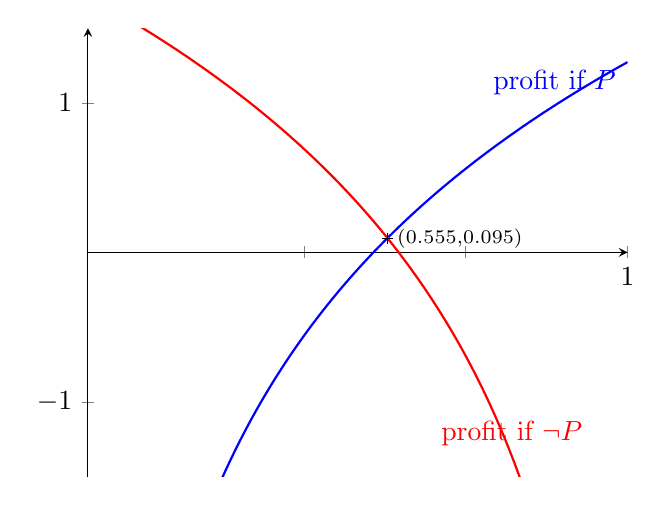
\begin{tikzpicture}
    \begin{axis}[
        axis lines=middle,
        xlabel=$\consp$,
        ylabel={},
        xmin=0, xmax=1,
        ymin=-1.5, ymax=1.5,
        %legend pos=outer north east,
        %clip=false,
        domain=0:1,
        samples=200,
        unbounded coords=jump, % Handling log(0) gracefully
        xtick={0, 0.4,0.7, 1.0},
        xticklabels={$0$,$\priceQ$, $\priceP$, $1$}
    ]
    \pgfmathdeclarefunction{s}{1}{\pgfmathparse{ln(#1)}}
    \addplot[blue, thick] {s(x) - s(0.7) + s(x) - s(0.4)} node[pos=0.97, above] {profit if $P$};
    \addplot[red, thick] {s(1-x) - s(1-0.7) + s(1-x) - s(1-0.4)} node[pos=0.15, above]{profit if $\lnot P$};

    %\legend{profit if $P$, profit if $\lnot P$}
    \addplot[only marks, mark=+, mark options={fill=black}] coordinates {(0.555, 0.095)}; % (0.5292,0) (0.5757,0)
    \node at (axis cs: 0.555, 0.095) [anchor=west] {$\scriptstyle{(0.555,0.095)}$};
    % \node at (axis cs: 0.5292, 0) [anchor=north]{$\scriptstyle{0.529}$};
    % \node at (axis cs: 0.5757, 0) [anchor=north]{$\scriptstyle{0.576}$};
    % \node at (axis cs: 0.7, 0) [anchor=south] {$P$};
    % \node at (axis cs: 0.4, 0) [anchor=south] {$Q$};
    \end{axis}
\end{tikzpicture}
\caption{Profit earned by the arbitrageur in case of inconsistency over ParaphraseChecker, taking $s(p)=\log(p)$ and $\priceP,\priceQ=0.7,0.4$ in \eqref{eq:profit-paraphrase}.}
\label{fig:profit-paraphrase}.
\end{figure}
% https://www.desmos.com/calculator/5kt8dkvr1e
% https://www.desmos.com/calculator/0fyuwmoasf

We may compute this intersection analytically:

\begin{align*}
    \score{\consp}-\score{\priceP}+\score{\consp}-\score{\priceQ} &=
    \score{1-\consp}-\score{1-\priceP}+\score{1-\consp}-\score{1-\priceQ} \\
    2\log\frac{\consp}{1-\consp}&=\log\frac{\priceP\priceQ}{(1-\priceP)(1-\priceQ)} \\
    \consp &= \frac{\sqrt{\priceP\priceQ}}{\sqrt{\priceP\priceQ}+\sqrt{(1-\priceP)(1-\priceQ)}} \\
\end{align*}

Substituting this back into either expression in \eqref{eq:profit-paraphrase} we get the expression for the arbitrage:

\begin{equation}
\Violation(\priceP,\priceQ)=-2\log\left(\sqrt{\priceP\priceQ}+\sqrt{(1-\priceP)(1-\priceQ)}\right)
\label{eq:arbitrage-paraphrase}
\end{equation}

As a bonus, this can straightforwardly be extended to the multi-question paraphrasing check: $(P_1\iff\dots\iff P_n)\implies(\Forecaster(P_1)=\dots=\Forecaster(P_n))$. Here the corresponding possible profits are:

\begin{equation}
\begin{cases}
    n\score{\consp}-\sum{\score{\Forecaster(P_i)}} & \text{if } P \\
    n\score{1-\consp}-\sum{\score{1-\Forecaster(P_i)}} & \text{if } \lnot P
\end{cases}
\label{eq:profit-paraphrase-multi}
\end{equation}

Equating them and solving for $\consp$, we get:

\begin{equation}
    \log\frac{p}{1-p}=\frac1n\sum_i\log\frac{\Forecaster(P_i)}{1-\Forecaster(P_i)}
    \label{eq:logodds-paraphrase-multi}
\end{equation}

\begin{equation}
    p=\frac{\Delta}{\Delta+1}
    \text{ where }
    \Delta=\left[\prod_i\frac{\Forecaster(P_i)}{1-\Forecaster(P_i)}\right]^{1/n}
    \label{eq:prob-paraphrase-multi}
\end{equation}

Observe that the arbitraged probability is simply the arithmetic mean in log-odds space! One may wonder if the violaton is some kind of variance measure in log-odds space, but this does not seem to be the case:

\begin{equation}
    \Violation(\Forecaster(P_1),\dots\Forecaster(P_n))=-n\log\left[
    \left(\prod\Forecaster(P_i)\right)^{1/n} +
    \left(\prod(1-\Forecaster(P_i))\right)^{1/n}
    \right]
    \label{eq:violation-paraphrase-multi}
\end{equation}

\subsubsubsection{NegChecker}
\label{apps:arbitrage-neg}

\NewDocumentCommand{\pricenotP}{}{\Forecaster(\lnot P)}

Suppose the forecaster produces forecasts $\Forecaster(P)$ and $\Forecaster(\lnot P)$. A trader who instead brings prices to $\Forecaster'(P)=\consp$, $\Forecaster'(\lnot P)=1-\consp$ earns a combined profit on both questions:

\begin{equation}
\begin{cases}
    \score{\consp}-\score{\priceP}+\score{\consp}-\score{1-\pricenotP} & \text{if } P \\
    \score{1-\consp}-\score{1-\priceP}+\score{1-\consp}-\score{\pricenotP} & \text{if } \lnot P
\end{cases}
\label{eq:profit-neg}
\end{equation}

Equating them and solving as before,

\begin{align*}
    2\log\frac{\consp}{1-\consp} &=
    \log\frac{\priceP(1-\pricenotP)}{(1-\priceP)\pricenotP} \\
    \consp &=
    \frac{\sqrt{\priceP(1-\pricenotP)}}{\sqrt{\priceP(1-\pricenotP)}+\sqrt{(1-\priceP)\pricenotP}} \\
\end{align*}

Substituting into \eqref{eq:profit-neg}, we get:

\begin{equation}
    \Violation(\priceP,\pricenotP)=-2\log\left(\sqrt{\priceP(1-\pricenotP)}+\sqrt{(1-\priceP)\pricenotP}\right)
\end{equation}

The similarity of these results to \ParaphraseChecker{} is suggestive: both the arbitraged probability and the violation for \NegChecker{} can be derived from \ParaphraseChecker{} simply replacing $\priceQ$ with $1-\pricenotP$, seeing the latter as the ``probability implied for $P$ by $\lnot P$''.
This raises the natural question: Can \emph{all} consistency checks be reduced to the case of \ParaphraseChecker{} arbitraging $\Forecaster(P)$ against an ``implied probability'' for $P$?

However, as we will see, \CondChecker{} shows that this approach does not always hold. Its violation expression depends on more than just $\Forecaster(P)$ and $\Forecaster(P\land Q)/\Forecaster(Q\mid P)$, so there is no single, neat interpretation akin to “arithmetic mean in the log-odds space.”

\subsubsubsection{CondChecker}

\NewDocumentCommand{\priceQgivenP}{}{\Forecaster(Q\mid P)}
\NewDocumentCommand{\pricePandQ}{}{\Forecaster(P\land Q)}
\NewDocumentCommand{\consq}{}{q}

Suppose the forecaster produces forecasts $\priceP$, $\priceQgivenP$, $\pricePandQ$. The possible outcomes $\Omega$ are $(P,Q\mid P,P\land Q)\mapsto$ $(\top,\top,\top)$, $(\top,\bot,\bot)$, $(\bot,\none,\bot)$. Consider an arbitrageur who makes bets $\Forecaster'(P)=\consp$, $\Forecaster'(Q\mid P)=\consq$, $\Forecaster'(P\land Q)=\consp\consq$.

In each outcome:

\begin{equation}
\begin{cases}
\score{\consp}-\score{\priceP}+\score{\consq}-\score{\priceQgivenP}+\score{\consp\consq}-\score{\pricePandQ}
& \mathrm{if } P,Q\\
\score{\consp}-\score{\priceP}+\score{1-\consq}-\score{1-\priceQgivenP}+\score{1-\consp\consq}-\score{1-\pricePandQ}
& \mathrm{if } P,\lnot Q\\
\score{1-\consp}-\score{1-\priceP}+\score{1-\consp\consq}-\score{1-\pricePandQ}
& \mathrm{if } \lnot P
\end{cases}
\label{eq:profit-cond}
\end{equation}

Equating these and rearranging:

\begin{equation*}
    \begin{cases}
    \frac{1-\consp}{\consp (1-\consq)} = \frac{1-\priceP}{\priceP(1-\priceQgivenP)} =: A\\
    \frac{1-\consq}{\consq}\frac{1-\consp\consq}{\consp\consq} = \frac{(1-\priceQgivenP)(1-\pricePandQ)}{\priceQgivenP\pricePandQ} =: B
    % \frac{\consp\consq^2}{(1-\consq)(1-\consp\consq)}=\frac{\priceQgivenP\pricePandQ}{(1-\priceQgivenP)(1-\pricePandQ)}\\
    % \frac{\consp(1-\consq)}{1-\consp}=\frac{\priceP(1-\priceQgivenP)}{1-\priceP}
    \end{cases}
\end{equation*}

Solving, where we indicate the right-hand-sides of each equation above by $A$ and $B$ respectively:

\begin{align*}
    \consp &= \frac{1 + \sqrt{B/(A+1)}}{1+\sqrt{B\cdot(A+1)}}\\
    \consq &= \frac{1}{1+\sqrt{B/(A+1)}}\\
    \consp\consq &= \frac{1}{1+\sqrt{B\cdot(A+1)}}
\end{align*}

Substituting back into \ref{eq:profit-cond} and simplifying:

\begin{align*}
&\Violation(\priceP,\priceQgivenP,\pricePandQ) \\ &= -2\log\left(\sqrt{\priceP\priceQgivenP\pricePandQ}+\sqrt{(1-\priceP\priceQgivenP)(1-\pricePandQ)}\right).
\end{align*}

% Solving, letting $X$ and $Y$ denote the right-hand sides of the first and second of the above equations:

% \begin{gather*}
%     \consq=1-\left(\frac{1}{\consp}-1\right)Y\\
%     X=\frac{1+Y(1-1/\consp)}{-Y(1-1/\consp)^2(1+Y)}\\
%     \dots\\
%     \frac{1}{\consp}-1 = \frac{Y+\sqrt{Y^2-4XY(1+Y)}}{2XY(1+Y)}\\
%     q=\frac{2X(1+Y)-Y-\sqrt{Y^2-4XY(1+Y)}}{2X(1+Y)}\\
%     p=\frac{2XY(1+Y)}{2XY(1+Y)+Y+\sqrt{Y^2-4XY(1+Y)}}\\
%     p=\frac{2XY(1+Y)+Y-\sqrt{Y^2-4XY(1+Y)}}{2(1+Y)(1+XY)}\\
%     pq=\frac{2XY-Y-\sqrt{Y^2-4XY(1+Y)}}{2(XY+1)}
% \end{gather*}
% Substituting back into any of \eqref{eq:profit-cond}:

% \subsubsubsection{CondChecker and CondCondChecker}

% The metric as stated does not quite work for conditional questions, because the arbitrageur is not rewarded at all for his bet on $Q\mid P$ if $P$ resolves False. Instead, this requires some ...

% Consider a standard Dutch book against an agent that gives probabilities $\Forecaster(Q|P)<\Forecaster(P\land Q)/\Forecaster(P)$:

% \begin{enumerate}
%     \item
% \end{enumerate}

\subsubsubsection{Numerical estimation}

Explicitly deriving the violation metrics for other checkers from \Cref{eq:arbitrage} is infeasible by hand, and the expressions yielded by SymPy are very convoluted. For these checks, we use a numerical algorithm based on solving a differential equation for $p_i(t)$, as detailed below.

The arbitraging process may be understood as adjusting market prices in such a way that the scores in each possible $\omega\in\Omega$ remain equal throughout the process -- i.e. such that their \emph{derivatives} remain equal. For derivatives $p_i'(t)$ of the prices, the derivatives of each score $s_\omega'(t)$ are:

\begin{equation*}
    s_\omega'(t)=
\begin{bmatrix}
    a_{\omega 1}(p_1) & \cdots & a_{\omega n}(p_n)
\end{bmatrix}
    \cdot
\begin{bmatrix}
    p_1'(t) \\
    \vdots \\
    p_n'(t)
\end{bmatrix}
\end{equation*}

Where

\begin{equation*}
a_{\omega i}(p_i) =
\begin{cases}
    s'(p_i) & \text{if } \omega_i = \top, \\
    -s'(1 - p_i) & \text{if } \omega_i = \bot, \\
    0 & \text{if } \omega_i = \None
\end{cases}
\end{equation*}

Then, where $A(\mathbf{p})=[a_{\omega i}(p_i)]$ (with $\Omega$ rows and $n$ columns), we have the derivative of the score vector $\mathbf{s}'(t)=A(\mathbf{p})\mathbf{p}'(t)$. We want $\mathbf{s}'(t)$ to be a multiple of $\begin{bmatrix}1 & \cdots & 1\end{bmatrix}$ to ensure it is the same in all outcomes $\omega$ -- the coefficient of proportionality does not matter (it just controls the ``speed'' at which you reach the arbitraged probabilities), so we can just solve $\mathbf{p}'(t)=A^{-1}\mathbf{s}'(t)$.

The dynamics of the arbitraging process are then simply:

\begin{equation*}
p_i(0) = \Forecaster(x_i)\quad\text{(initial conditions)}
\end{equation*}

\begin{equation*}
\mathbf{p}'(t) = A(\mathbf{p})^{-1}\begin{bmatrix}
    1 \\ \vdots \\ 1
\end{bmatrix}
\end{equation*}

Which we run until $\det A$ reaches 0, which is when consistency is reached.

% \subsubsubsection{Numerical estimation}

% Explicitly deriving the violation metrics for other checkers from \Cref{eq:arbitrage} is infeasible by hand, and the expressions yielded by SymPy are very convoluted.
% Instead, we compute the violation numerically for all consistency checks, i.e. use a global optimizer to compute the max.
% The global maximization algorithm we use is \emph{shgo}, introduced in \cite{endresSimplicialHomologyAlgorithm2018}, as provided by SciPy; other methods we found to be equally effective were \emph{differential\_evolution} \cite{stornDifferentialEvolutionSimple1997} and \emph{dual\_annealing} \cite{xiangGeneralizedSimulatedAnnealing2013}.
% %
% The pseudocode for computing arbitrage
% is given in Algorithm~\ref{alg:numerical}.
% %\todo{I feel like this is redundant overexplaining but IDK}

% \algnewcommand{\LeftComment}[1]{\(\triangleright\) #1}
% \NewDocumentCommand{\forecast}{}{f}
% \MakeRobust{\Call}

% \begin{algorithm}[tb]
% \caption{Numerical computation of \Cref{eq:arbitrage}}
% \label{alg:numerical}
% \begin{algorithmic}

% \Procedure{Arbitrage}{$\Resolution,\forecast,p$}
% \State\LeftComment{Computes the profit earned by an arbitrageur who bets $p\in[0,1]^n$ against forecasts $\forecast\in[0,1]^n$ upon an $n$-tuple of questions resolving as $\Resolution\in\ResolutionsOpt^n$}
% \State Initialize $s\gets 0$
% \For{$i\in\{1\dots n\}$}
% \If{$\Resolution(i)=\none$}
% \State continue
% \EndIf
% \If{$\Resolution(i)=\top$}
% \State $s\gets s + s(p(i))-s(\forecast(i))$
% \EndIf
% \If{$\Resolution(i)=\bot$}
% \State $s\gets s + s(1-p(i))-s(1-\forecast(i))$
% \EndIf
% \EndFor
% \State return $s$
% \EndProcedure

% \Procedure{MinArbitrage}{$\forecast,p$}
% \State\LeftComment{Minimizes \Call{Arbitrage}{$\Resolution,\forecast,p$} over all $\Resolution$s that satisfy $\Relation$}
% \State $\ResolutionsVec:=\{\resolutionvec\in\ResolutionsOpt^n\mid\Relation(\resolutionvec)\}$\Comment{All $\Resolutions$ that satisfy the consistency check $\Relation$}
% \State return $\min_{\Resolution\in\ResolutionsVec}\Call{Arbitrage}{\Resolution,\forecast,p}$\Comment{Minimization over a finite set}
% \EndProcedure

% \Procedure{MaxMinArbitrage}{$\forecast$}
% \State\LeftComment{Maximizes \Call{MinArbitrage}{$\forecast,p$} over all possible arbitrageur bets $p$, i.e. calculates the arbitrageur's optimal bet and its profit thereof}

% \State Initialize $p\gets\forecast$ \Comment{Initial guess}
% \State $D\gets [\epsilon,1-\epsilon]^n$ \Comment{Avoid $\log(0)$}

% \State $p,v\gets\Call{GlobalMaximization}{\Call{MinArbitrage}{\forecast,p}}$\Comment{maximize over $p$}

% \State return $p$, $v$
% \EndProcedure

% \end{algorithmic}
% \end{algorithm}


\newcommand{\betamin}{\beta_{\textsc{min}}}

\subsubsection{Frequentist consistency metric}
\label{cfc/app:frequentist-metric}
\todo{maybe change P to x throughout here too}
In a deterministic world, we cannot let any inconsistency pass; every time we prove any rule of probability does not hold exactly, we must discard the forecaster as flawed.
This is too strict for the consistency check framework to be useful.
Instead, we propose a violation metric and the corresponding inconsistency threshold based on statistical hypothesis testing.\todo{make equations break properly}

Assume that each event $P$ has a true probability value $\TrueProb(P)$, say under some world model that accounts for aleatoric uncertainty.
\begin{definition}[Frequentist consistency]
\label{def:frequentist-consistency}
A frequentist-consistent forecaster $\Forecaster$ samples a Gaussian estimate $\TrueProb(P) + \eps$ of each event $P$, with variance $\sigma^2 \TrueProb(P) (1 - \TrueProb(P))$ for a hyperparameter $\sigma^2$:
\begin{align}
    \label{eq:frequentist_consistency}
    \Forecaster(P) - \TrueProb(P) \sim \Normal\left(0, \sigma^2 \TrueProb(P) (1 - \TrueProb(P))\right) \quad \text{independently for all events } P.
\end{align}
\end{definition}
This is principled from the frequentist perspective.
Consider a forecaster that just samples the (relevant subset of) the world $n$ times using the best available world simulator, and estimates the probability of each event $P$ as the proportion of times that $P$ occurs in the $n$ samples.
If we estimate the probability as the average chance of an event $P$ with true probability $p$ occurring out of $n$ times, then this estimate has a scaled binomial distribution with mean $p$ and variance $p(1-p) / n$.
To reach \Cref{eq:frequentist_consistency}, replace the averaged binomial with the Gaussian of the same variance, and denote $\sigma^2 := 1/n$.


This simple model enables us to derive hypothesis tests for each of the consistency checks described in \Cref{tab:consistency_checks}.
The null hypothesis is always that the forecaster is frequentist-consistent.
Note that $\sigma^2$ is not our estimate of the variance of any forecaster; it is just a hyperparameter that controls how strict our null hypothesis is.
We leave estimating the variance of a particular forecaster and testing frequentist consistency based on that alone to future work.

\paragraph{Notation}
The expression $a \Normal(0, c^2)$ denotes a Gaussian random variable with mean 0 and variance $a^2 c^2$.
The expression $a \Normal(0, c^2) + b \Normal(0, c^2)$ denotes a Gaussian random variable with mean 0 and variance $a^2 c^2 + b^2 c^2$.
All sums range over the cyclic permutations of the variables under the sum.
All $\Normal(0, c^2)$ terms appearing with the same power of $\sigma$ are independent.
Two $\Normal(0, c^2)$ terms appearing with a different power of $\sigma$ may be correlated; this is not important for our purposes, since we discard high-order powers of $\sigma$.

\paragraph{Bootstrapping the true probability}
The final expressions for hypothesis test statistics might involve the true probability $\TrueProb(P)$.
It is not available, so we just plug in $\Forecaster(P)$ for $\TrueProb(P)$ in the end.
If we had a prior on $\TrueProb(P)$, we could combine it with $\Forecaster(P)$ to get a more robust estimate.


\paragraph{\NegChecker}
We take the violation metric and the corresponding threshold as to produce a hypothesis test against this:
\begin{align*}
   \Forecaster(P) + \Forecaster(\neg P) - 1
   = \TrueProb(P) + \eps_1 + \TrueProb(\neg P) + \eps_2 - 1
   = \eps_1 + \eps_2
   \\
   \sim \Normal\left(0, \sigma^2 (\TrueProb(P)(1 - \TrueProb(P)) + \TrueProb(\neg P)(1 - \TrueProb(\neg P))) \right)
\end{align*}


We estimate the unknown $\TrueProb$ values with the corresponding $\Forecaster$ estimates.  Note that, although $\TrueProb(P) = 1- \TrueProb(\neg P)$, it is of course not necessarily the case that $\Forecaster(P) = 1- \Forecaster(\neg P)$.

The error distribution is $\sigma \Normal\left( \Forecaster(P) (1 - \Forecaster(P)) + \Forecaster(\neg P) (1 - \Forecaster(\neg P)) \right)$, and the two-sided test is
\begin{align*}
   \abs{\Forecaster(P) + \Forecaster(\neg P) - 1} < \gamma \sigma \sqrt{(1 - \Forecaster(P)) \Forecaster(P) + (1 - \Forecaster(\neg P)) \Forecaster(\neg P)}
\end{align*}
for some scale factor $\gamma$ (number of standard deviations) that scales the power of the test. For example, $\gamma = 2.58$ gives a 99\%-confidence interval.

We now want to compute some \emph{consistency violation metric} that makes inconsistency comparable across different checks. The natural idea is to aggregate all terms dependent on $\Forecaster$ to one side; and make the hypothesis test be just some threshold on the computed violation metric.

It is possible that the denominator of the resulting expression is $0$ when the forecaster is certain and $\Forecaster$ is $0$ or $1$; to avoid division with zero, we add a small regularization term $\betamin = 10^{-3}$.
See the last paragraph of this section for a discussion of hyperparameters.

Our consistency violation metric is then:
\begin{align*}
    v_{\NegChecker}
    = \frac{\abs{\Forecaster(P) + \Forecaster(\neg P) - 1}}{\sqrt{(1 - \Forecaster(P)) \Forecaster(P) + (1 - \Forecaster(\neg P)) \Forecaster(\neg P) + \betamin}}.
\end{align*}

The hyperparameter $\sigma^2$ determines how strict we are with rejecting inconsistencies which could be attributed to ``noisy'' predictions. Note that the violation metric itself does not depend on $\sigma^2$.

A violation (inconsistency), therefore, occurs when:
\begin{align*}
    v_{\NegChecker} > \gamma \sigma.
\end{align*}

\paragraph{\CondCondChecker}
This is a more complex consistency check; we derive the hypothesis test and violation metric in detail below. For the other checks, we just report the short derivation.

\begin{align*}
(a, b, c, d) &= \left(\TrueProb(P), \TrueProb(Q \mid P), \TrueProb(R \mid P \wedge Q), \TrueProb(P \wedge Q \wedge R)\right) \\
(a', b', c', d') &= \left(\Forecaster(P), \Forecaster(Q \mid P), \Forecaster(R \mid P \wedge Q), \Forecaster(P \wedge Q \wedge R)\right)
\end{align*}

We can write:

\begin{align*}
    \Forecaster(P) &= \Normal\left(0, \sigma^2 a (1 - a)\right) + a, \\
    \Forecaster(Q\mid P) &= \Normal\left(0, \sigma^2 b (1 - b)\right) + b, \\
    \Forecaster(R \mid P \wedge Q) &= \Normal\left(0, \sigma^2 c (1 - c)\right) + c, \\
    \Forecaster(P \wedge Q \wedge R) &= \Normal\left(0, \sigma^2 d (1 - d)\right) + d
\end{align*}

We now compute the difference of the two expressions that should be equal.
All sums and products are cyclic over $a$, $b$, $c$.
%, we can compute where $i,j,k$ cyclically take on the values of $a,b,c$
%\begin{align*}
%    \Forecaster(P) \Forecaster(Q \mid P) \Forecaster(R \mid P \wedge Q) - \Forecaster(P \wedge Q \wedge R) &= abc - d \\
%    &+ \sigma \left( \sum jk \Normal(0, i(1-i)) - \Normal(0, d(1-d))\right) \\
%    &+ \sigma^2 \sum i \Normal(0, j(1-j)) \Normal(0, k(1-k)) \\
%    &+ \sigma^3 \prod \Normal(0, i(1-i))
%\end{align*}
\begin{align*}
    \Forecaster(P) \Forecaster(Q \mid P) \Forecaster(R \mid P \wedge Q) - \Forecaster(P \wedge Q \wedge R)
    &= abc - d \\
    &+ \sigma \left( \sum_{a} bc \Normal(0, a(1-a)) - \Normal(0, d(1-d))\right) \\
    &+ \sigma^2 \sum_{a} \Normal(0, b(1-b)) \Normal(0, c(1-c)) \\
    &+ \sigma^3 \prod_{a} \Normal(0, a(1-a)).
\end{align*}

In the above, all Gaussians with the same variance are identical, and all other combinations are independent.
As $abc - d = 0$ by the law of total probability, the leading error term is next to $\sigma$.
This is a Gaussian with mean 0 and standard deviation:

\begin{align*}
    \sigma \sqrt{\sum_{a} b^2c^2 a(1-a) + d(1-d)}
    =
    \sigma \sqrt{abc \sum_{a} bc (1-a) + d(1-d)}
\end{align*}
\todo{this expression could be simplified, it's already simplified in code}



We now discard the terms of $\sigma^2$, $\sigma^3$, and in general any higher order power of $\sigma$. This is principled because the coefficients can always be (in some confidence interval) upper bounded by a constant independent of $\sigma$.
Hence, if $\sigma$ is small enough, the resulting test will be very close to the true hypothesis test.



We do not have the true probabilities $a$, $b$, $c$, $d$, so we just plug in $(a', b', c', d') = (\Forecaster(P), \Forecaster(Q \mid P), \Forecaster(R \mid P \wedge Q), \Forecaster(P \wedge Q \wedge R))$. \footnote{Depending on how we use the relation $abc=d$, we can end up with different expressions in the end. We choose the one that, after plugging in, (i) yields an expression for variance that is always nonnegative, and (ii) is not a polynomial multiple of any single value of $\Forecaster$.}
 Thus the hypothesis test is (where the sum is cyclic over $a'$, $b'$, $c'$):

\begin{align*}
    \abs{a'b'c' - d'}
    > \gamma \sigma \sqrt{ a' b' c' \sum_{a'} b'c' (1-a') + d' (1-d')}
\end{align*}

Our violation metric is then:
\begin{align*}
    v_{\CondCondChecker}
    = \frac{
        \abs{a'b'c' - d'}
        }{
        \sqrt{a'b'c' \sum_{a'} b'c' (1-a') + d' (1-d')+ \betamin}
    }.
\end{align*}
where again $(a', b', c', d') = (\Forecaster(P), \Forecaster(Q \mid P), \Forecaster(R \mid P \wedge Q), \Forecaster(P \wedge Q \wedge R))$ are the forecasts.


\paragraph{\CondChecker}

Similarly as for \CondCondChecker: we denote
$(a, b, c) = \left(\TrueProb(P),  \TrueProb(P \mid Q), \TrueProb(P \wedge Q) \right)$ and the associated $(a', b', c')$ for the forecasts.
Then we can compute
\begin{align*}
    &\Forecaster(P) \Forecaster(Q \mid P) - \Forecaster(P \wedge Q) \\
    &= ab - c + \sigma \left(b \Normal(0, a(1-a)) + a \Normal(0, b(1-b)) - \Normal(0, c(1-c)) \right) \\
    &\quad + \sigma^2 \Normal(0, a(1-a)) \Normal(0, b(1-b)).
\end{align*}

% \begin{align*}
%     &\Forecaster(P) \Forecaster(Q \mid P) - \Forecaster(P \wedge Q)
%     \\ &= ab - c
%     + \sigma \left(b \Normal(0, a(1-a) + a \Normal(0, b(1-b)) - \Normal(0, c(1-c)) \right)
%     + \sigma^2 \Normal(0, a(1-a)) \Normal(0, b(1-b)).
% \end{align*}



The term next to $\sigma$ is a Gaussian with mean 0 and standard deviation:

\begin{align*}
    \sigma \sqrt{a^2 b(1-b) + b^2 a(1-a) + c(1-c)}
    = \sigma \sqrt{ab \left( a(1-b) + b(1-a) \right) + c(1-c)}.
\end{align*}

Again, we have to plug in $(a', b', c') = (\Forecaster(P), \Forecaster(Q \mid P), \Forecaster(P \wedge Q))$ instead of $(a, b, c)$.

Our violation metric is then:
\begin{align*}
    v_{\CondChecker}
    = \frac{\abs{a'b' - c'}}{
        \sqrt{a'b' \left( a'(1-b') + b'(1-a') \right) + c'(1-c')+ \betamin}
    }
\end{align*}
And the test is again, for a suitable $\gamma$ corresponding to the desired power of the test:
\begin{align*}
    v_{\CondChecker} > \gamma \sigma.
\end{align*}


\paragraph{\ParaphraseChecker}

Here we can simply check whether $P$ and $Q$ are the same.

\begin{align*}
   &\Forecaster(P) - \Forecaster(Q)
   = \TrueProb(P) + \eps_1 - \TrueProb(Q) - \eps_2 \\
   &= \eps_1 - \eps_2 \sim \Normal\left(0, \sigma^2 ((\TrueProb(P)(1 - \TrueProb(P)) + (\TrueProb(Q)(1 - \TrueProb(Q)) \right)
\end{align*}

This yields the following violation metric:

\begin{align*}
    v_{\ParaphraseChecker}
    = \frac{\abs{\Forecaster(P) - \Forecaster(Q)}}{
        \sqrt{(\Forecaster(P)(1 - \Forecaster(P)) + (\Forecaster(Q)(1 - \Forecaster(Q))+ \betamin}
    }
\end{align*}

\paragraph{\AndOrChecker}

\begin{align*}
   &\Forecaster(P) + \Forecaster(Q) - \Forecaster(P \lor Q) - \Forecaster(P \land Q) \\
   & =
   \TrueProb(P) + \TrueProb(Q) - \TrueProb(P \lor Q) - \TrueProb(P \land Q) + \eps_1 + \eps_2 - \eps_3 - \eps_4 \\
   &= \eps_1 + \eps_2 - \eps_3 - \eps_4 \\
   &\sim \Normal\left(0, \sigma^2 \left( \TrueProb(P)(1 - \TrueProb(P)) + \TrueProb(Q)(1 - \TrueProb(Q)) \right. \right. \\
   &\left. \left. + \TrueProb(P \lor Q)(1 - \TrueProb(P \lor Q)) + \TrueProb(P \land Q)(1 - \TrueProb(P \land Q)) \right) \right).
\end{align*}


% \begin{align*}
%    &\Forecaster(P) + \Forecaster(Q) - \Forecaster(P \lor Q) - \Forecaster(P \land Q) \\
%    & =
%    \TrueProb(P) + \TrueProb(Q) - \TrueProb(P \lor Q) - \TrueProb(P \land Q) + \eps_1 + \eps_2 - \eps_3 - \eps_4 \\
%    &= \eps_1 + \eps_2 - \eps_3 - \eps_4 \\
%    &\sim \Normal\left(0, \sigma^2 ((\TrueProb(P)(1 - \TrueProb(P)) + (\TrueProb(Q)(1 - \TrueProb(Q)) \\
%    &+ (\TrueProb(P \lor Q)(1 - \TrueProb(P \lor Q)) + (\TrueProb(P \land Q)(1 - \TrueProb(P \land Q))) \right).
% \end{align*}

We again plug in $\Forecaster$ instead of $\TrueProb$ to compute the error term allowed: $\gamma \sigma \sqrt{M}$ where

\begin{align*}
    &M = \Forecaster(P)(1 - \Forecaster(P)) + \Forecaster(Q)(1 - \Forecaster(Q) + \Forecaster(P \lor Q)(1 - \Forecaster(P \lor Q)) + \\
    &\Forecaster(P \land Q)(1 - \Forecaster(P \land Q))
\end{align*}

and violation metric:

\begin{align*}
    v_{\AndOrChecker}
    = \frac{\abs{\Forecaster(P) + \Forecaster(Q) - \Forecaster(P \lor Q) - \Forecaster(P \land Q)}}{
        \sqrt{\begin{array}{l}
            \Forecaster(P)(1 - \Forecaster(P)) + \Forecaster(Q)(1 - \Forecaster(Q)) + \\
            \Forecaster(P \lor Q)(1 - \Forecaster(P \lor Q)) + \Forecaster(P \land Q)(1 - \Forecaster(P \land Q)) + \betamin
        \end{array}}
    }.
\end{align*}

\paragraph{\ButChecker}

\begin{align*}
   &\Forecaster(P \lor Q) - \Forecaster(P) - \Forecaster(\lnot P \land Q) =
   \TrueProb(P \lor Q) - \TrueProb(P) - \TrueProb(\lnot P \land Q) + \eps_1 - \eps_2 - \eps_3 =\\
   &\eps_1 - \eps_2 - \eps_3 \sim\\
   &\Normal\left(0, \sigma^2 ((\TrueProb(P \lor Q)(1 - \TrueProb(P \lor Q)) + (\TrueProb(P)(1 - \TrueProb(P)) + (\TrueProb(\lnot P \land Q)(1 - \TrueProb(\lnot P \land Q)) \right)
\end{align*}

with error term:

\begin{align*}
    \gamma \sigma \sqrt{\Forecaster(P \lor Q)(1 - \Forecaster(P \lor Q) + \Forecaster(P)(1 - \Forecaster(P) + \Forecaster(\lnot P \land Q)(1 - \Forecaster(\lnot P \land Q)}
\end{align*}

and violation metric:

\begin{align*}
    v_{\ButChecker}
    = \frac{\abs{\Forecaster(P \lor Q) - \Forecaster(P) - \Forecaster(\lnot P \land Q)}}{
        \sqrt{\Forecaster(P \lor Q)(1 - \Forecaster(P \lor Q)) + \Forecaster(P)(1 - \Forecaster(P)) + \Forecaster(\lnot P \land Q)(1 - \Forecaster(\lnot P \land Q)+ \betamin}
    }
\end{align*}


\paragraph{\ConsequenceChecker}

In the case of inequalities involving $\le$, there are two ways in which the consistency check can be passed.
If $\Forecaster(P) \le \Forecaster(Q)$, the consistency check is automatically passed.
Otherwise,
we check for pseudo-equality using the same violation metric as in \ParaphraseChecker.

\begin{align*}
    v_{\ConsequenceChecker}
    = [\Forecaster(P) > \Forecaster(Q)] \frac{\abs{\Forecaster(P) - \Forecaster(Q)}}{
        \sqrt{\Forecaster(P)(1 - \Forecaster(P)) + \Forecaster(Q)(1 - \Forecaster(Q))+ \betamin}
    }
\end{align*}
where $[\Forecaster(P) > \Forecaster(Q)]$ is the Iverson Bracket (1 if true, 0 otherwise).

%\textbf{Note: Adam  Not sure if we should include changing $\gamma = 2$}

%The only difference is that the hypothesis test is one-sided; therefore, $\gamma$ needs to be smaller to get the same confidence interval.
%We choose $\gamma = 2$ by default for one-sided tests, to get a level of around 97\% similar as for $\gamma = 3$ in \ParaphraseChecker.

\paragraph{\AndChecker}


Similarly to \ConsequenceChecker, if the chain of strict inequalities
\begin{align*}
    \max(\Forecaster(P) + \Forecaster(Q) - 1, 0) < \Forecaster(P \land Q) < \min(\Forecaster(P), \Forecaster(Q))
\end{align*}
holds, then the check automatically passes.  We set $v_{\AndChecker\_\textsc{lhs}} = 0$ and $v_{\AndChecker\_\textsc{rhs}} = 0$ if it passes the first and second strict inequality respectively.

If not, then we test for pseudo-equality for the violating pair:

$\text{LHS}: \max(\Forecaster(P)+\Forecaster(Q)-1, 0) = \Forecaster(P\land Q)$

$ \text{RHS}: \Forecaster(P\land Q)  = \min(\Forecaster(P),\Forecaster(Q))$

Equality check if it fails the first inequality:

\begin{align*}
    \eps_{\textsc{lhs}} = \begin{dcases*}
        \gamma\sigma
        \sqrt{\Forecaster(P)(1-\Forecaster(P))+\Forecaster(Q)(1-\Forecaster(Q)) + \Forecaster(P\land Q)(1-\Forecaster(P\land Q))} \\
        \quad \text{if } \Forecaster(P)+\Forecaster(Q)-1 > 0, \\[6pt]
        \text{N/A} \\
        \quad \text{otherwise pass as } \Forecaster(P\land Q) \ge 0.
    \end{dcases*}
\end{align*}





\begin{align*}
    v_{\AndChecker\_\textsc{lhs}}
    &= [\Forecaster(P) + \Forecaster(Q) - 1 > \Forecaster(P\land Q)] \cdot \\ &\frac{
            \Forecaster(P) + \Forecaster(Q) - 1 - \Forecaster(P \land Q)
    }{
        \sqrt{\Forecaster(P)(1-\Forecaster(P))+\Forecaster(Q)(1-\Forecaster(Q)) + \Forecaster(P\land Q)(1-\Forecaster(P\land Q))+ \betamin}
    }
\end{align*}

Equality check if it fails the second inequality:

Define $\Forecaster(R) =  \min(\Forecaster(P),\Forecaster(Q))$.

\begin{align*}
    \eps_{\textsc{rhs}}
    &=  \gamma\sigma\sqrt{
        \Forecaster(P\land Q)(1-\Forecaster(P\land Q))+\Forecaster(R)(1+\Forecaster(R))
    }
    \\
    v_{\AndChecker\_{\textsc{rhs}}}
    &= [\Forecaster(R) < \Forecaster(P\land Q)] \frac{
            \Forecaster(P \land Q) - \Forecaster(R)
    }{
        \sqrt{\Forecaster(P\land Q)(1-\Forecaster(P\land Q)) + \Forecaster(R)(1-\Forecaster(R))+ \betamin}
    }
\end{align*}


Consistency is violated if either inequality is violated, \emph{and} the respective hypothesis test for pseudo-equality fails. We use $v_{\AndChecker\_\textsc{lhs}}$ for the first and $v_{\AndChecker\_\textsc{rhs}}$ for the second inequality.
We define $v_{\AndChecker} = \max\{v_{\AndChecker\_\textsc{lhs}}, v_{\AndChecker\_\textsc{rhs}} \}$.



\paragraph{\OrChecker}

We proceed similarly as for \AndChecker{}.

If the strict inequality $\max(\Forecaster(P),\Forecaster(Q))<\Forecaster(P\lor Q)<\min(1,\Forecaster(P)+\Forecaster(Q))$ holds, then it automatically passes.  We set $v_{\OrChecker\_\textsc{lhs}} = 0$ and $v_{\OrChecker\_\textsc{rhs}} = 0$ if it passes the first and second strict inequality respectively.

If not, we test for pseudo-equality:

$\text{LHS}: \max(\Forecaster(P),\Forecaster(Q)) = \Forecaster(P\lor Q)$

$\text{RHS}: \Forecaster(P\lor Q) = \min(1,\Forecaster(P)+\Forecaster(Q))$.


Equality check LHS:
Define  $\Forecaster(S) =  \max(\Forecaster(P),\Forecaster(Q))$.
\begin{align*}
    &\eps_{\textsc{lhs}} =
        \gamma\sigma\sqrt{\Forecaster(S)(1-\Forecaster(S)) + \Forecaster(P\lor Q)(1-\Forecaster(P\lor Q))}
\end{align*}

\begin{align*}
    v_{\OrChecker\_{\textsc{lhs}}}
    = [\Forecaster(S) > \Forecaster(P\lor Q)] \frac{
      \Forecaster(S) - \Forecaster(P \lor Q)
    }{
      \sqrt{\Forecaster(S)(1-\Forecaster(S)) + \Forecaster(P\lor Q)(1-\Forecaster(P\lor Q)) + \betamin}
    }
\end{align*}

Equality check RHS:

\begin{align*}
    \eps_{\textsc{rhs}} = \begin{dcases*}
        \gamma\sigma\sqrt{\Forecaster(P\lor Q)(1-\Forecaster(P\lor Q)) + \Forecaster(P)(1-\Forecaster(P)) + \Forecaster(Q)(1-\Forecaster(Q))} \\
        \quad \text{if } \Forecaster(P)+\Forecaster(Q) < 1, \\[6pt]
        \text{N/A} \\
        \quad \text{otherwise pass as } \Forecaster(P\lor Q) \le 1.
    \end{dcases*} \\
\end{align*}
\begin{align*}
    v_{\OrChecker\_{\textsc{rhs}}}
    &= [\Forecaster(P) + \Forecaster(Q) < \Forecaster(P\lor Q)] \cdot \\ & \quad{} \frac{
            \Forecaster(P\lor Q) - \Forecaster(P) - \Forecaster(Q)
    }{
        \sqrt{\Forecaster(P\lor Q)(1-\Forecaster(P\lor Q)) + \Forecaster(P)(1-\Forecaster(P)) + \Forecaster(Q)(1-\Forecaster(Q))+ \betamin}
    }
\end{align*}

Consistency is violated if either inequality is violated, \emph{and} the subsequent hypothesis test for pseudo-equality fails. We use $v_{\OrChecker\_\textsc{lhs}}$ for the first and  $v_{\OrChecker\_\textsc{rhs}}$ for the second inequality.
Analogously to \AndChecker{}, define $v_{\OrChecker} = \max\{v_{\OrChecker\_\textsc{lhs}}, v_{\OrChecker\_\textsc{rhs}} \}$.

\paragraph{\ExpectedEvidenceChecker}
\label{cfc/app:frequentist-ee}

Write $(a,b,c,d)=(\TrueProb(P),\TrueProb(P\mid Q),\TrueProb(P\mid\lnot Q), \TrueProb(Q))$; then

\begin{align*}
& b'd'+c'(1-d')-a' \\
& =
(b + \sigma N(b(1-b)))(d + \sigma N(d(1-d)))
\\ & \quad +
(c + \sigma N(c(1-c)))(1 - d - \sigma N(d(1-d)))
\\ & \quad - (a+\sigma N(a(1-a))) \\
& = (bd+c(1-d)-a)
\\ & \quad + \sigma \left[
d N(b(1-b))\right. \\
&\quad\quad + (b-c) N(d(1-d)) \\
&\quad\quad + (1-d)N(c(1-c)) \\
&\left.\quad\quad - N(a(1-a))
\right]
\\ & \quad + O(\sigma^2) \\
\end{align*}

gives us a normal distribution with standard deviation

\begin{equation*}
\sigma\sqrt{
a(1-a)
+ d^2 b (1-b)
+ (1-d)^2 c (1-c)
+ (b-c)^2 d (1-d).
}
\end{equation*}

The violation metric is then:

\begin{equation*}
\frac{
|bd+c(1-d)-a|
}{
\sigma\sqrt{
a(1-a)
+ d^2 b (1-b)
+ (1-d)^2 c (1-c)
+ (b-c)^2 d (1-d).
}
}
\end{equation*}

\paragraph{Hyperparameters for hypothesis testing}
\label{cfc/app:frequentist-hyperparams}
Our goal is for the rejection criteria to be similar to the arbitrage violation metric in \Cref{cfc/app:arbitrage} on simple examples.
We choose $\gamma = 2.58$ for all checks, to ensure 99\%-confidence intervals for two-sided tests;
future work may consider using a different $\gamma$ for checks that require one-sided tests.
We pick $\sigma = 0.05$ (corresponding to $n = 400$ in \Cref{def:frequentist-consistency}).
The allowed violation threshold for all checks is then $\gamma \sigma = 0.129$.
For reference, a \NegChecker{} pair $(\Forecaster(P), \Forecaster(\neg P)) = (0.5, 0.59)$ has a violation metric of $0.128$, and would thus not be rejected as inconsistent.
This \rebuttal{closely} corresponds to the tolerance threshold of $10^{-2}$ of profit for the arbitrage metric, described in \Cref{cfc/sec:consistency-checks-intro}.

We pick $\betamin = 10^{-3}$ because LLM forecasters from \citet{halawiApproachingHumanLevelForecasting2024} answer with at most 3 digits of precision for events close to $0$ and $1$ in probability.



%\subsubsection{Tolerance scaling, [0, 1] space}
%
%\todo{this and the Adam section below need to be cleaned up}
%
%Assume that each event $P$ has a true probability value $\TrueProb(P)$. Take the null hypothesis:
%
%$\Forecaster$ produces a Gaussian estimate of each event $P$ centered at $\TrueProb(P)$, with variance $\sigma^2$ uniform across all events:
%
%\begin{align*}
%    \Forecaster(P) - \TrueProb(P) \sim \Normal(0, \sigma^2) \quad \text {independently for all events } P
%\end{align*}
%
%We take the violation metric and the corresponding threshold as to produce a hypothesis test against this:
%\begin{align*}
%   \Forecaster(P) + \Forecaster(\neg P) - 1
%   = \TrueProb(P) + \eps_1 + \TrueProb(\neg P) + \eps_2 - 1
%   = \eps_1 + \eps_2 \sim \Normal(0, 2\sigma^2)
%\end{align*}
%
%
%\subsubsection{Tolerance scaling, log space}
%For high or low probabilities, it is more principled to assume $\log \Forecaster$ produces a Gaussian estimate of the \emph{log prob}:
%
%\begin{align*}
%   \frac{\Forecaster(P)}{\TrueProb(P)} \sim \exp(\Normal(0, \sigma^2)) \quad
%    \text {independently for all events } P
%\end{align*}
%
%\dpaleka{Maybe it will be beneficial to have two sets of metrics reported, one behaving well for log error and one behaving well for linear error. Then make sure that those are both benevolent outside the intervals where they make sense, and reject consistency if at least one of them fails.}
%
%\todo{Adam's comment:  in practice log makes sense when we have a distribution bounded by 0 on one side and inf on the other..  Linear makes sense if left is unbounded and right is unbounded.  For prediction markets [0,1 bounds] something like logistic makes most sense}
%
%
%
%$$\exp(\varepsilon_1)\TrueProb(P)+\exp(\varepsilon_2)(1-\TrueProb(P))
%=\TrueProb(P)(\exp(\varepsilon_1)-\exp(\varepsilon_2))+\exp(\varepsilon_2) ???
%$$
%no wait the test statistic would actually be something else right not exactly $\Forecaster(P)+\Forecaster(\lnot P)-1$
%
%
%
%e.g., in the negation case log(p/(1-p))+log(q/(1-q)) has a distribution of
%
%$$\log\frac{X}{1-e^\varepsilon+X}$$
%
%where
%
%$X=e^{2\varepsilon}p^*(1-p^*)$

%\subsubsection{Asking LLM for confidence intervals and using Z-Scores as Violation Checker (Adam's methods)}\todo{this should be commented out no?}
%
%To determine the consistency of large language model (LLM) predictions, it is necessary to elicit not only prediction probabilities, but also confidence intervals. A more confident prediction should be associated with tighter violation tolerances, whereas looser confidence intervals indicate the model's understanding of its own uncertainty, allowing for more forgiving tolerances.
%
%As mentioned in \ref{cfc/sec:tolerance-scaling freq}, one method to ascertain a model's true prediction and confidence intervals is through a frequentist approach, which involves querying the LLM $n$ times and aggregating its outputs to estimate an average $\mu$ and a standard deviation $\sigma$ of its predictions. However, a key weakness of this approach is its assumption that the production of estimates from the LLM constitutes independent experiments. This assumption is flawed because, although LLMs are generally programmed to generate varied responses, the underlying data and architecture on which they are trained remain constant for each query. An analogous situation would be for a social scientist conducting a survey among 100 individuals regarding a prediction market event; there is a significant difference between querying 100 distinct individuals and querying a single individual 100 times.
%
%Consequently, the frequentist approach tends to underestimate the true $\sigma$ and confidence interval of the model. Since prediction events are singular and have not yet occurred, it is impossible to statistically construct accurate confidence intervals using past data. A feasible workaround is to directly ask the LLM model "What is your 1 $\sigma$ confidence interval for your previous prediction?" Similarly to human market participants and traders, this direct approach examines not only the accuracy and consistency of the model's predictions, but also its ability to comprehend uncertainty and probability ranges within a singular, unified framework.
%
%
%\subsubsubsection{Z-Score Tolerance Scoring}
%
%Another way to score consistency and tolerance is by utilizing the Z-score method.  Here we compare the amount of violation with the total expected confidence bounds that the model gave for its original predictions: $Z = \abs{\frac{\text{Violation}}{\sigma_{tot}}}$.  We can define $Z>1$ as a violation.
%
%Using the example of a modified negation checker, we separate $2\sigma^2$ to $\sigma_{orig}^2 \text{and} \sigma_{neg}^2 $, which are the associated stated confidence intervals that the LLM answers when asked for the original prediction and the negated prediction.  From there we calculate $Z = \frac{\eps_1 + \eps_2}{\sqrt{\sigma_{orig}^2 + \sigma_{neg}^2}}$.
%
%\begin{align*}
%   \Forecaster(P) + \Forecaster(\neg P) - 1
%   = \TrueProb(P) + \eps_1 + \TrueProb(\neg P) + \eps_2 - 1
%   = \eps_1 + \eps_2 \sim \Normal(0, {\sigma_{orig}}^2 + {\sigma_{neg}}^2)
%\end{align*}
%



%NegChecker: $\CCheck(\Forecaster(P),\Forecaster(\lnot P)):=\Forecaster(P)+\Forecaster(\lnot P)=1$; violation metric: $\Violation(\Forecaster(P),\Forecaster(\lnot P)) = |\Forecaster(P)+\Forecaster(\lnot P)-1|$.
%
%AndOrChecker: $\CCheck(\Forecaster(P),\Forecaster(Q),\Forecaster(P\land Q),\Forecaster(P\lor Q)):=\Forecaster(P)+\Forecaster(Q)=\Forecaster(P\lor Q)+\Forecaster(P\land Q)$; violation metric: $\Violation(\Forecaster(P),\Forecaster(Q),\Forecaster(P\land Q),\Forecaster(P\lor Q)) = |\Forecaster(P)+\Forecaster(Q)-\Forecaster(P\land Q)-\Forecaster(P\lor Q)|$.
%
%AndChecker. $\CCheck(\Forecaster(P),\Forecaster(Q),\Forecaster(P\land Q)):=\max(\Forecaster(P)+\Forecaster(Q)-1, 0) \le \Forecaster(P\land Q) \le \min(\Forecaster(P),\Forecaster(Q))$; violation metric: $\Violation(\Forecaster(P),\Forecaster(Q),\Forecaster(P\land Q)):=\max(\max(\Forecaster(P)+\Forecaster(Q)-1, 0)-\Forecaster(P\land Q), \Forecaster(P\land Q)-\min(\Forecaster(P),\Forecaster(Q))
%
%OrChecker: $\CCheck(\Forecaster(P),\Forecaster(Q),\Forecaster(P\lor Q)):=\max(\Forecaster(P),\Forecaster(Q))\le\Forecaster(P\lor Q)\le\min(1,\Forecaster(P)+\Forecaster(Q))$
%
%ButChecker: $\CCheck(\Forecaster(P),\Forecaster(\lnot P\land Q),\Forecaster(P\lor Q)):=\Forecaster(P\lor Q)=\Forecaster(P)+\Forecaster(\lnotP\land Q)$; violation metric: $\Violation(\Forecaster(P),\Forecaster(\lnot P\land Q),\Forecaster(P\lor Q)):=|\Forecaster(P)+\Forecaster(\lnot P\land Q)-\Forecaster(P\lor Q)|$.
%
%SymmetryAndChecker: $\CCheck(\Forecaster(P\land Q),\Forecaster(Q\land P)):=\Forecaster(P\land Q)=\Forecaster(Q\land P)$; violation metric: $\Violation(P\land Q,Q\land P)=|\Forecaster(P\land Q)-\Forecaster(Q\land P)|$
%SymmetryOrChecker: $\CCheck(\Forecaster(P\lor Q),\Forecaster(Q\lor P)):=\Forecaster(P\lor Q)=\Forecaster(Q\lor P)$; violation metric: $\Violation(P\lor Q,Q\lor P)=|\Forecaster(P\lor Q)-\Forecaster(Q\lor P)|$
%CondChecker: $\CCheck(\Forecaster(P),\Forecaster(Q|P),\Forecaster(P\land Q)); violation metric: $\Violation(\Forecaster(P),\Forecaster(Q|P),\Forecaster(P\land Q)):=\Forecaster(P)\Forecaster(Q|P)-\Forecaster(P\land Q)$.
%
%CondCondChecker: $\CCheck(\Forecaster(P), \Forecaster(Q|P), \Forecaster(R|P\land Q), \Forecaster(P\land Q\land R)):=\Forecaster(P)\Forecaster(Q|P)\Forecaster(R|P\land Q)=\Forecaster(P\land Q\land R)$; violation metric: \Violation(\Forecaster(P), \Forecaster(Q|P), \Forecaster(R|P\land Q), \Forecaster(P\land Q\land R))=\Forecaster(P)\Forecaster(Q|P)\Forecaster(R|P\land Q)-\Forecaster(P\land Q\land R)$
%
%ConsequenceChecker: (where $\Relation(P,Q):=P\implies Q$) $\CCheck(P,Q):=\Forecaster(P)\le\Forecaster(Q)$; violation metric: $\Violation(P,Q):=\max(\Forecaster(P)-\Forecaster(Q),0)$
%
%ParaphraseChecker (where $\Relation(P,Q):=P\iff Q$) $\CCheck(P,Q):=\Forecaster(P)=\Forecaster(Q)$; violation metric: $\Violation(P,Q)=|\Violation(P)-\Violation(Q)|$
\subsubsection{\CFCaster{}}
\label{cfc/app:cfcaster}

To formally define \CFCaster{}, we need to first formalize our ``instantiation'' process mathematically:

\begin{definition}[Tuple sampler]
Let $\Relation:\ForecastingQuestions^n\to\bools$, $\CCheck:\Forecasts^n\to\bools$ be a consistency check. Then we call $\FullInstantiator:\ForecastingQuestions\rightsquigarrow\ForecastingQuestions^n$ a ``single-base-question tuple sampler'' for $\Relation$ if for all $x$, $\FullInstantiator(x)_1=x$ and $\Relation(\FullInstantiator(x))$ holds surely.
\label{def:instantiator}
\end{definition}

A multiple-base-question tuple sampler $\Instantiator:\ForecastingQuestions^m\to\ForecastingQuestions^n$, like our instantiation process, can simply be composed with a question sampler $\Generator:\ForecastingQuestions\rightsquigarrow\ForecastingQuestions$ (e.g a synthetic generator or a sampler from our dataset) to produce a single-base-question sampler $\FullInstantiator(x):=\Instantiator(x,\Generator(x),\dots\Generator(x))$.

Next, in order to correctly handle sequentially arbitraging checks and prevent bias towards later applied checks, we need to introduce ``weighted'' arbitraging. This follows easily from Eq~\ref{def:arbitrage} by simply having the scoring rule for each question $x$ be $w_x\log(p)$. We denote the calculation of arbitraged probabilities under these weighted scoring rules by $\Arbitrageur^{(w_1,\dots w_n)}$.

\begin{definition}[\CFCaster{}]
Let $\Forecaster:\ForecastingQuestions\to\Forecasts$ be the ``Base Forecaster'', and let $\vec{C}:=[(\Relation_1,\CCheck_1,\FullInstantiator_1),...(\Relation_k,\CCheck_k,\FullInstantiator_k)]$ be a list of consistency checks along with respective single-base-question tuple samplers. Then we construct a new forecaster $\CFC[\vec{C}]{\Forecaster}:\ForecastingQuestions\to\Forecasts$ that produces its forecast for a given question $x$ as given in Algorithm~\ref{alg:cf}; we call this the \CFCaster{} with base $\Forecaster$ and check list $\vec{C}$.

\begin{algorithm}[tb]
\caption{\CFCaster{} algorithm: $\CFC[\vec{C}]{\Forecaster}$}
\label{alg:cf}
\begin{algorithmic}

\State \textbf{input} $x$
\State $p\gets\Forecaster(x)$\Comment{Query base forecaster}
\State $w\gets 1$
\For{$(\Relation_i,\CCheck_i,\FullInstantiator_i)$ in $\vec{C}$}

\State $(x,x_2,\dots x_n) \gets \FullInstantiator_i(x)$\Comment{Instantiate tuple of size $n=n_{\Relation_i}$}
\State $(p_2,\dots p_n) \gets (\Forecaster(x_2),\dots\Forecaster(x_n))$\Comment{Query base forecaster on tuple}
\State $(p,p_2,\dots p_n) \gets \Arbitrageur_i^{(w,1,\dots 1)}(p,p_2,\dots p_n)$\Comment{arbitrage the forecasts as per Def~\ref{eq:arbitrage}}
\State $w\gets w+n-1$\Comment{$p$ now carries information from $n-1$ other markets}
\EndFor
\State\Return p

\end{algorithmic}
\end{algorithm}

\label{def:cf}
\end{definition}

The first thing we observe is that this isn't necessarily \emph{robust} to different instantiations. For this reason, we a priori expect that \textbf{\CFCaster{} will be more effective on }

% Note that despite our original hope, it is \emph{not} true that $\CFC[\vec{C}]{\Forecaster}$ is definitionally consistent on the checks in $\vec{C}$, even if $\vec{C}$ contains only a single consistent check. Instead we must study the performance of \CFCaster{} empirically. Furthermore, we can apply \CFCaster{} recursively to itself, i.e. $\CFC[\vec{C}_1]{\CFC[\vec{C}_2]{\Forecaster}}$ and so on -- in particular for the case $\vec{C}_1=\dots \vec{C}_r$, we denote $\CFC[\vec{C}]{\Forecaster}^r:=\CFC[\vec{C}]{\CFC[\vec{C}]{\Forecaster}^{r-1}}$.

% Appendix~\ref{cfc/app:cfcaster} contains theoretical details on the consistency of \CFCaster{} as well as the motivation for studying this recursive forecaster.



\NewDocumentCommand{\checktriple}{}{(\Relation,\CCheck,\FullInstantiator)}

We might hope that the \CFCaster{} introduced in Def~\ref{def:cf} would be definitionally consistent on the checks it is arbitraged on. However, this is not the case \emph{even for }\CFCaster{}\emph{ applied to a single check} $\Relation(x_1,\dots x_n)$,  because the tuple of forecasts that is arbitraged to compute $\CFC[\checktriple]{\Forecaster}(x_1)$, the tuple arbitraged to compute $\CFC[\checktriple]{\Forecaster}(x_2)$, \ldots, the tuple arbitraged to compute $\CFC[\checktriple]{\Forecaster}(x_n)$ are all different. While the tuple instantiated to compute $\CFC[\checktriple]{\Forecaster}(x_1)$ could indeed be $\FullInstantiator(x_1)=(x_1,\dots x_n)$ (at least if the tuple sampler $\FullInstantiator$ is deterministic and happens to be the same as the one used in the instantiation of the check), the tuples instantiated to compute $\CFC[\checktriple]{\Forecaster}(x_i)$ for $i\ne 1$ will be $\FullInstantiator(x_i)$, all of which are different from one another.

\NewDocumentCommand{\para}{}{\operatorname{para}}
\NewDocumentCommand{\negate}{}{\operatorname{neg}}

To make this concrete, consider the simplest case of $\CFC[P]{\Forecaster}$ (where $P$ is short for \ParaphraseChecker{}); let $\para$ be a deterministic tuple-sampler for $\ParaphraseChecker{}$. $\CFC[P]{\Forecaster}(x)$ is calculated by arbitraging $\Forecaster(x)$ and $\Forecaster(\para(x))$. But $\Forecaster(\para(x))$ is calculated by arbitraging $\Forecaster(\para(x))$ and $\Forecaster(\para(\para(x)))$.

A priori, this gives us the following hypothesis: \textbf{\CFCaster{} will be especially effective for fundamentally ``symmetric'' checks like \NegChecker{}} -- where $\negate(\negate(P))$ is likely to be a very similar sentence to $P$. Although we have not conducted a full scale experiment of \CFCaster{} with each checker, our preliminary results in Table~\ref{tab:cf-nx} do suggest very good performance of \CFCaster{} on \NegChecker{}.

Suppose, however, that we had an ``extended'' \CFCaster{} that made its forecast for $x$ based on the tuple $(x,\para(x),\para^2(x),\dots \para^r(x))$ -- then its forecast for $\para(x)$ would be based on $(\para(x),\para^2(x),\dots\para^{r+1}(x)$ -- these tuples would be ``almost'' the same, except with $\para^{r+1}(x)$ instead of $x$, and this extended \CFCaster{} would be ``almost'' consistent on \ParaphraseChecker{}.

This is precisely the idea behind recursively applying \CFCaster{} to itself: we recursively define $\CFC{\Forecaster}^r(x):=\Arbitrageur(\CFC{\Forecaster}^{r-1}(\FullInstantiator(x)_i)\text{ for }i=1,\dots n)$ -- then \emph{if} this iteration approaches a fixed point, this fixed point $\CFC{\Forecaster}^\infty$ is consistent. More precisely:

\begin{theorem}[Consistency of recursive \CFCaster{}]
\label{thm:recursive}
Let $\checktriple$ be an $n$-ary consistency check and a corresponding deterministic tuple sampler satisfying Def~\ref{def:instantiator}, and have $\Arbitrageur(p_1,\dots p_n)$ and $\Violation(p_1,\dots p_n)$ denote the arbitraging function and arbitrage metric corresponding to $\Relation$ as per Def~\ref{def:arbitrage} under a logarithmic scoring rule. Then, for some ``base forecaster'' $\CFC{\Forecaster}^0=\Forecaster$, recursively define

\begin{equation*}
\CFC{\Forecaster}^r(x):=\Arbitrageur(\CFC{\Forecaster}^{r-1}(\FullInstantiator(x)_i)\text{ for }i=1,\dots n)
\end{equation*}

If this iteration converges pointwise in log-odds space -- i.e. if for all $x\in\ForecastingQuestions$, the sequence $\CFC{\Forecaster}^r(x)$ has a limit strictly between 0 and 1, then $\Violation(\CFC{\Forecaster}^r(\FullInstantiator(x)_i)\text{ for }i=1,\dots n)\to 0$.
%If this iteration converges pointwise in log-odds space -- i.e. if for all $x\in\ForecastingQuestions$, the sequence $\log\frac{\CFC{\Forecaster}^r(x)}{1-\CFC{\Forecaster}^r(x)}$ converges as $r\to\infty$, then $\Violation(\CFC{\Forecaster}^r(\FullInstantiator(x)_i)\text{ for }i=1,\dots n)\to 0$.
\end{theorem}
\begin{proof}
Recall as per Def~\ref{def:arbitrage} that, where $\Omega$ is the set of possible outcomes allowed by $\Relation$:
\begin{align*}
&\Violation(\CFC{\Forecaster}^r(\FullInstantiator(x)_i)\text{ for }i=1,\dots n)\\
&=\min_{\omega\in\Omega}\sum_{i=1}^n \left(\log(\Arbitrageur(\CFC{\Forecaster}^r(\FullInstantiator(x)_j)\text{ for }j=1,\dots n)_i)-\log\CFC{\Forecaster}^r(\FullInstantiator(x)_i)\right)\delta_{\omega(i)=\top}\\
&\quad+
\left(\log(1-\Arbitrageur(\CFC{\Forecaster}^r(\FullInstantiator(x)_j)\text{ for }j=1,\dots n)_i)-\log(1-\CFC{\Forecaster}^r(\FullInstantiator(x)_i))\right)\delta_{\omega(i)=\bot}\\
&=\min_{\omega\in\Omega}\sum_{i=1}^n \left(\log\CFC{\Forecaster}^{r+1}(\FullInstantiator(x)_i))-\log\CFC{\Forecaster}^r(\FullInstantiator(x)_i)\right)\delta_{\omega(i)=\top}\\
&\quad+
\left(\log(1-\CFC{\Forecaster}^{r+1}(\FullInstantiator(x)_i)-\log(1-\CFC{\Forecaster}^r(\FullInstantiator(x)_i))\right)\delta_{\omega(i)=\bot}
\end{align*}

Since $\CFC{\Forecaster}^r(x)$ converges to something that is neither 0 nor 1, so do $\log\CFC{\Forecaster}^r(x)$ and $\log(1-\CFC{\Forecaster}^r(x))$. And as this is true for \emph{all} $x$, so in particular it is true for $\FullInstantiator(x)_i$. Thus the expression above is a finite sum of terms that each approach 0.
\end{proof}\todo{idk if this result should be a "theorem" tbh.}

This is a somewhat weak result: other than for \NegChecker{} and \ParaphraseChecker{}, none of our static consistency checks involved a deterministic instantiation process -- they all require sampling other related base questions, and having the checks use the same instantiation process as the \CFCaster{} would be cheating.

\NewDocumentCommand{\logodds}{}{\log\operatorname{odds}}

Furthermore, this gives us no actual conditions for the convergence of the iteration. At least for \ParaphraseChecker{}, we have the following -- where $\logodds p$ denotes $\log\frac{p}{1-p}$:

\begin{theorem}[Convergence of recursive \CFCaster{} for \ParaphraseChecker{}]
If the sequence $a_i=\logodds\Forecaster(\para^i(x))$ is convergent, then the condition of Theorem~\ref{thm:recursive} holds for the recursive \CFCaster{} defined arbitraged on \ParaphraseChecker{} with tuple sampler $\para$.
\end{theorem}
\begin{proof}
Recall from Sec~\ref{apps:checks-paraphrase} that the arbitraged probability for \ParaphraseChecker{} is simply the average of the original probabilities in log-odds space, i.e. $\logodds\Arbitrageur(\Forecaster(x),\Forecaster(\para(x)))=\frac{\logodds\Forecaster(x)+\logodds\Forecaster(\para(x))}{2}$. We can apply this recursively to get:
\begin{equation*}
\CFC{\Forecaster}^r(x)=\frac{1}{2^r}\sum_{i=0}^r{\binom{r}{i}\logodds\Forecaster(\para^i(x))}
\end{equation*}
Which is simply a binomial moving average of $\logodds\Forecaster(\para^i(x))=a_i$, and converges iff $a_i$ does. Convergence in log-odds space is equivalent to convergence of probability to something other than 0 or 1, so the result follows.
\end{proof}

\subsubsubsection{Choices of experiments}
\label{cfc/app:cfcaster-cost}
A single call to $\CFC[\vec{C}]{\Forecaster}$, where $\vec{C}:=[(\Relation_1,\CCheck_1,\FullInstantiator_1),...(\Relation_k,\CCheck_k,\FullInstantiator_k)]$, involves $1+\sum_i (n_{\Relation_i}-1)$ calls to $\Forecaster$, plus at least $\sum_i(m_{\Relation_i}+n_{\Relation_i}-2)$ (where $m_{\Relation_i}$ is the number of separate base questions that must be generated synthetically in each tuple) LLM calls for the $\FullInstantiator_i$s.

For all the checks listed in Table~\ref{tab:consistency_checks}, this amounts to a total of 49 LLM calls per question. For a \emph{recursive} \CFCaster{} set-up of depth $r$, this amounts to $49^r$ LLM calls per question, which can get prohibitively expensive. Even on \gptfouromini{} and assuming $\approx 600$ input tokens and 600 output tokens on average, this amounts to $\approx\$0.02$ per question at depth $r=1$, and $\approx\$2500$ per question at depth $r=4$.

Furthermore, it was not clear that experimenting on all checks made logical sense: recursive \CFCaster{} set-ups with \CondChecker{}, \CondCondChecker{} and \ExpectedEvidenceChecker{} would involve forms like $P\mid(Q\mid R)$, which do not have a basis in probability theory. We decided to prioritize studying the following hypotheses and research questions, motivated by the theoretical discussion above:

\begin{enumerate}
    \item We hypothesised above that \CFCaster{} will be \textbf{particularly effective on checks that are symmetric and have deterministic instantiations} -- thus we studied $\CFC[\NegChecker{}]{\gptfouromini{}}$.
    \item We hypothesized that there would be \textbf{consistency gains from increasing depth $r$} -- thus we studied recursive \CFCaster{} setups on \NegChecker{} an \ParaphraseChecker{}, where it was most practical to.
    \item We were interested to know \textbf{if the consistency gains observed when arbitraging on one check alone would persist after arbitraging on a sequence of checks} -- to predict if this would hold when arbitraging on the full sequence of checks, we did a preliminary run of $\CFC[\NegChecker{},\ParaphraseChecker{}]{\gptfouromini{}}$ and tested if it maintains consistency on \NegChecker{} and \ParaphraseChecker{}.
    \item \textbf{We expected $\CFC[\ExpectedEvidenceChecker{}]{\Forecaster}$ to improve ground truth and consistency scores across the board.} This is based on our intuition that arbitraging on \ExpectedEvidenceChecker{} essentially ``informs'' the forecast on a question $x$ with consideration information $y$ -- except instead of subjectively feeding this information (e.g. in chain-of-thought), it adjusts for it via a strict probabilistic rule. Although a recursive setup would not make sense for \ExpectedEvidenceChecker{}, $\CFC[[\ExpectedEvidenceChecker{}]*r]{\Forecaster}$ simply sequentially arbitrages on \ExpectedEvidenceChecker{} repeatedly (breaking the seed each time to ensure unique new questions $y$), which amounts to informing the forecast for $x$ with information $y_1$, $y_2$ etc.
\end{enumerate}

The results reported in Sec~\ref{cfc/sec:cfcaster} of the main body and \ref{cfc/app:cf-results} of the Appendix provide evidence in favour of hypotheses 1 and 2, answer 3 in the affirmative, and do not provide clear evidence on 4.

Future work should compare $\CFC[[\ExpectedEvidenceChecker{}]]{\Forecaster}$ against a comparable chain-of-thought model in which the forecaster is asked to consider these related questions before it makes its forecast.\manyu{not sure if this is a good idea to write; this is basically the PromptToConsForecaster that we didn't get to work}

\subsubsubsection{Results tables for \CFCaster{}}
\label{cfc/app:cf-results}

Consistency violation and ground truth results for each of the \CFCaster{} configurations we experimented with are reported in Tables~\ref{tab:cf-nx},~\ref{tab:cf-px},~\ref{tab:cf-npx}~and~\ref{tab:cf-ee}. The results included are for the NewsAPI dataset and the arbitrage metric.
Results for the scraped and 2028 synthetic datasets, as well as for the
frequentist metric, look very similar; they are available in the supplementary data of this paper.

{
\setlength{\tabcolsep}{0.46em}
\begin{table}[htbp]
\caption{Consistency results (arbitrage metric) for $\CFC[\NegChecker{}]{\gptfouromini{}}^r$ (denoted CF-Nr) forecasters on NewsAPI questions.}
%\caption{Average violation and fraction of consistency violations for each $\CFC[\NegChecker{}]{\gptfouromini{}}^r$ (denoted CF-Nr) on NewsAPI questions. Consistency on \NegChecker{} is significantly improved compared to the base forecaster, but its performance on other checks varies by check, with slightly worse performance on aggregate consistency and no significant difference on ground truth performance.}
\begin{tabular}{lrrrrrrrrrr}
\toprule
Check & \multicolumn{2}{c}{\gptfouromini{}} & \multicolumn{2}{c}{CF-N1} & \multicolumn{2}{c}{CF-N2} & \multicolumn{2}{c}{CF-N3} & \multicolumn{2}{c}{CF-N4} \\
 & Avg & Frac & Avg & Frac & Avg & Frac & Avg & Frac & Avg & Frac \\
\midrule
\NegChecker{} & 0.036 & 43\% & 0.012 & 33\% & 0.007 & 22\% & 0.004 & 11\% & 0.004 & 9\% \\
\ParaphraseChecker{} & 0.013 & 27\% & 0.012 & 36\% & 0.008 & 23\% & 0.006 & 16\% & 0.005 & 17\% \\
\CondCondChecker{} & 0.084 & 85\% & 0.111 & 88\% & 0.121 & 91\% & 0.129 & 94\% & 0.136 & 93\% \\
\ExpectedEvidenceChecker{} & 0.015 & 27\% & 0.009 & 35\% & 0.008 & 25\% & 0.007 & 26\% & 0.007 & 25\% \\
\ConsequenceChecker{} & 0.005 & 10\% & 0.003 & 9\% & 0.003 & 7\% & 0.002 & 4\% & 0.001 & 3\% \\
\AndChecker{} & 0.006 & 20\% & 0.019 & 45\% & 0.027 & 53\% & 0.031 & 59\% & 0.035 & 65\% \\
\OrChecker{} & 0.007 & 13\% & 0.004 & 10\% & 0.002 & 6\% & 0.002 & 6\% & 0.001 & 4\% \\
\AndOrChecker{} & 0.017 & 38\% & 0.024 & 58\% & 0.031 & 61\% & 0.033 & 67\% & 0.035 & 66\% \\
\ButChecker{} & 0.053 & 75\% & 0.081 & 84\% & 0.091 & 89\% & 0.100 & 88\% & 0.107 & 91\% \\
\CondChecker{} & 0.062 & 88\% & 0.085 & 92\% & 0.107 & 91\% & 0.119 & 94\% & 0.131 & 96\% \\
aggregated & 0.030 &  & 0.036 &  & 0.041 &  & 0.043 &  & 0.046 &  \\
Brier score & 0.185 &  & 0.204 &  & 0.202 &  & 0.201 &  & 0.201 &  \\
\bottomrule
\end{tabular}
\label{tab:cf-nx}
\end{table}


\begin{table}[htbp]
\caption{Consistency results (arbitrage metric) for $\CFC[\ParaphraseChecker{}]{\gptfouromini{}}^r$ (denoted CF-Pr) forecasters on NewsAPI questions.}
% \caption{Average violation and fraction of consistency violations for each $\CFC[\ParaphraseChecker{}]{\gptfouromini{}}^r$ (denoted CF-Pr) on NewsAPI questions. Consistency on \ParaphraseChecker{} is significantly improved compared to the base forecaster, but its performance on other checks varies, with slightly better performance on aggregate consistency and no significant difference on ground truth performance.}
\begin{tabular}{lrrrrrrrrrr}
\toprule
Check & \multicolumn{2}{c}{\gptfouromini{}} & \multicolumn{2}{c}{CF-P1} & \multicolumn{2}{c}{CF-P2} & \multicolumn{2}{c}{CF-P3} & \multicolumn{2}{c}{CF-P4} \\
 & Avg & Frac & Avg & Frac & Avg & Frac & Avg & Frac & Avg & Frac \\
\midrule
\NegChecker{} & 0.036 & 43\% & 0.028 & 49\% & 0.026 & 50\% & 0.023 & 46\% & 0.024 & 44\% \\
\ParaphraseChecker{} & 0.013 & 27\% & 0.006 & 22\% & 0.004 & 11\% & 0.002 & 6\% & 0.002 & 3\% \\
\CondCondChecker{} & 0.084 & 85\% & 0.083 & 83\% & 0.079 & 85\% & 0.080 & 83\% & 0.079 & 84\% \\
\ExpectedEvidenceChecker{} & 0.015 & 27\% & 0.014 & 28\% & 0.012 & 24\% & 0.011 & 28\% & 0.012 & 28\% \\
\ConsequenceChecker{} & 0.005 & 10\% & 0.002 & 4\% & 0.001 & 3\% & 0.001 & 2\% & 0.001 & 2\% \\
\AndChecker{} & 0.006 & 20\% & 0.004 & 12\% & 0.005 & 13\% & 0.004 & 12\% & 0.004 & 12\% \\
\OrChecker{} & 0.007 & 13\% & 0.005 & 10\% & 0.004 & 9\% & 0.003 & 10\% & 0.003 & 9\% \\
\AndOrChecker{} & 0.017 & 38\% & 0.015 & 41\% & 0.014 & 42\% & 0.013 & 39\% & 0.013 & 39\% \\
\ButChecker{} & 0.053 & 75\% & 0.053 & 76\% & 0.049 & 77\% & 0.051 & 79\% & 0.048 & 79\% \\
\CondChecker{} & 0.062 & 88\% & 0.066 & 93\% & 0.071 & 95\% & 0.069 & 95\% & 0.071 & 95\% \\
aggregated & 0.030 &  & 0.028 &  & 0.026 &  & 0.026 &  & 0.026 &  \\
Brier score & 0.185 &  & 0.176 &  & 0.175 &  & 0.174 &  & 0.175 &  \\
\bottomrule
\end{tabular}
\label{tab:cf-px}
\end{table}

\begin{table}[htbp]
\caption{Consistency results (arbitrage metric) for $\CFC[[\NegChecker{},\ParaphraseChecker{}]]{\gptfouromini{}}^r$ (denoted CF-NPr) forecasters on NewsAPI questions.}
% \caption{Average violation and fraction of consistency violations for each $\CFC[[\NegChecker{},\ParaphraseChecker{}]]{\gptfouromini{}}^r$ (denoted CF-NPr) on NewsAPI questions. Consistency on both \NegChecker{} and \ParaphraseChecker{} are significantly improved compared to the base forecaster, and similar to CF-Nr and CF-Pr alone, but its performance on other checks varies, with no significant difference on aggregate consistency or ground truth performance.}
\begin{tabular}{lrrrrrrrrrr}
\toprule
Check & \multicolumn{2}{c}{\gptfouromini{}} & \multicolumn{2}{c}{CF-NP1} & \multicolumn{2}{c}{CF-NP2} & \multicolumn{2}{c}{CF-NP3} & \multicolumn{2}{c}{CF-NP4} \\
 & Avg & Frac & Avg & Frac & Avg & Frac & Avg & Frac & Avg & Frac \\
\midrule
\NegChecker{} & 0.036 & 43\% & 0.014 & 30\% & 0.007 & 18\% & 0.004 & 9\% & 0.003 & 6\% \\
\ParaphraseChecker{} & 0.013 & 27\% & 0.006 & 17\% & 0.003 & 7\% & 0.002 & 2\% & 0.001 & 2\% \\
\CondCondChecker{} & 0.084 & 85\% & 0.095 & 90\% & 0.096 & 86\% & 0.108 & 94\% & 0.115 & 94\% \\
\ExpectedEvidenceChecker{} & 0.015 & 27\% & 0.010 & 27\% & 0.007 & 27\% & 0.006 & 22\% & 0.005 & 21\% \\
\ConsequenceChecker{} & 0.005 & 10\% & 0.003 & 7\% & 0.001 & 3\% & 0.001 & 2\% & 0.001 & 0\% \\
\AndChecker{} & 0.006 & 20\% & 0.011 & 30\% & 0.010 & 28\% & 0.011 & 34\% & 0.012 & 39\% \\
\OrChecker{} & 0.007 & 13\% & 0.004 & 11\% & 0.002 & 5\% & 0.001 & 4\% & 0.001 & 2\% \\
\AndOrChecker{} & 0.017 & 38\% & 0.017 & 43\% & 0.016 & 46\% & 0.016 & 46\% & 0.016 & 47\% \\
\ButChecker{} & 0.053 & 75\% & 0.070 & 85\% & 0.072 & 91\% & 0.077 & 91\% & 0.083 & 97\% \\
\CondChecker{} & 0.062 & 88\% & 0.082 & 96\% & 0.076 & 97\% & 0.076 & 97\% & 0.077 & 98\% \\
aggregated & 0.030 &  & 0.031 &  & 0.029 &  & 0.030 &  & 0.031 &  \\
Brier score & 0.185 &  & 0.188 &  & 0.195 &  & 0.200 &  & 0.202 &  \\
\bottomrule
\end{tabular}
\label{tab:cf-npx}
\end{table}


\begin{table}[htbp]
\caption{Consistency results (arbitrage metric) for $\CFC[[\ExpectedEvidenceChecker{}]*r]{\gptfouromini{}}$ \\(denoted CF-rxEE1) forecasters on NewsAPI questions.}
% \caption{Average violation and fraction of consistency violations for each $\CFC[[\ExpectedEvidenceChecker{}]*r]{\gptfouromini{}}$ (denoted CF-rxEE1) on NewsAPI questions. There is a modest improvement across all consistency checks, as well as on ground truth, compared to the base forecaster; however there are diminishing returns to arbitraging repeatedly on multiple \ExpectedEvidenceChecker{} tuples.}
\begin{tabular}{lrrrrrrrrrr}
\toprule
% Check & \multicolumn{2}{c}{\gptfouromini{}} & \multicolumn{2}{c}{$\CFC[[E]]{\gptfouromini{}}$} & \multicolumn{2}{c}{$\CFC[2*[E]]{\gptfouromini{}}$} & \multicolumn{2}{c}{$\CFC[3*[E]]{\gptfouromini{}}$} & \multicolumn{2}{c}{$\CFC[4*[E]]{\gptfouromini{}}$} \\
Check & \multicolumn{2}{c}{\gptfouromini{}} & \multicolumn{2}{c}{CF-1xEE1} & \multicolumn{2}{c}{CF-2xEE1} & \multicolumn{2}{c}{CF-3xEE1} & \multicolumn{2}{c}{CF-4xEE1} \\
 & Avg & Frac & Avg & Frac & Avg & Frac & Avg & Frac & Avg & Frac \\
\midrule
\NegChecker{} & 0.036 & 43\% & 0.030 & 51\% & 0.026 & 49\% & 0.024 & 50\% & 0.025 & 53\% \\
\ParaphraseChecker{} & 0.013 & 27\% & 0.008 & 22\% & 0.006 & 22\% & 0.005 & 19\% & 0.005 & 18\% \\
\CondCondChecker{} & 0.084 & 85\% & 0.057 & 82\% & 0.053 & 79\% & 0.050 & 76\% & 0.044 & 74\% \\
\ExpectedEvidenceChecker{} & 0.015 & 27\% & 0.008 & 22\% & 0.007 & 19\% & 0.007 & 16\% & 0.007 & 20\% \\
\ConsequenceChecker{} & 0.005 & 10\% & 0.003 & 8\% & 0.002 & 7\% & 0.002 & 5\% & 0.002 & 6\% \\
\AndChecker{} & 0.006 & 20\% & 0.002 & 6\% & 0.002 & 6\% & 0.002 & 4\% & 0.001 & 5\% \\
\OrChecker{} & 0.007 & 13\% & 0.004 & 9\% & 0.003 & 8\% & 0.002 & 8\% & 0.003 & 9\% \\
\AndOrChecker{} & 0.017 & 38\% & 0.014 & 42\% & 0.011 & 39\% & 0.010 & 34\% & 0.011 & 35\% \\
\ButChecker{} & 0.053 & 75\% & 0.040 & 71\% & 0.039 & 74\% & 0.040 & 77\% & 0.035 & 68\% \\
\CondChecker{} & 0.062 & 88\% & 0.049 & 88\% & 0.046 & 89\% & 0.044 & 88\% & 0.040 & 87\% \\
aggregated & 0.030 &  & 0.021 &  & 0.020 &  & 0.019 &  & 0.017 &  \\
Brier score & 0.185 &  & 0.172 &  & 0.171 &  & 0.171 &  & 0.173 &  \\
\bottomrule
\end{tabular}
\label{tab:cf-ee}
\end{table}
}


% \section*{Reproducibility Statement}
% We include the questions, forecasting results, and consistency results necessary to reproduce all tables and plots in the paper. The forecasts data \footnote{\url{https://github.com/dpaleka/consistency-forecasting/tree/b093e5134f219ca4d82720bb996ec1fb850024ae/src/data/forecasts}} is organized by forecaster, with two directories for each forecaster:

% \begin{enumerate}
%     \item Ground truth forecasting results:
%     \begin{itemize}
%         \item JSONL file, where each entry has (question, boolean resolution, forecast,  per-question Brier score, metadata and reasoning traces)
%         \item JSON file: total Brier score, calibration, other metrics
%     \end{itemize}

%     \item Consistency checks results:
%     \begin{itemize}
%         \item JSONL file with raw results, where each entry (questions, forecasts, consistency violations, metadata and reasoning traces)
%         \item JSON file: summary statistics (e.g., average violation)
%     \end{itemize}
% \end{enumerate}

% The consistency check results directories have a substring \texttt{tuples} in the directory name. For the 2028 synthetic dataset, we have only the consistency check result directories.

% \end{appendix}
